\documentclass[Master,Final,ngerman,UKenglish,twoside]{scrbook}
%------------------------------------------------------------------------------
% This file contains a skeleton thesis for
% a Physics or Astronomy Institute in the University of Bonn

% Specify the thesis type as an option: PhD, Master, Diplom, Bachelor
% Specify the thesis stage as an option: Draft (default), Submit, Final, PILibrary

% Specify the language(s) in the class and then use babel.
% If you need more than one language, give the default language last,
% e.g. ngerman,UKenglish for a thesis in British (UK) English where you want
% to be able to set the language to German for some part of it.
\textwidth15.0cm

%------------------------------------------------------------------------------
% Pass TeX Live version to the package
% Use command pdflatex --version to find out which version you are running
% Add option backref=false when your thesis is ready to turn off back-referencing
% in your bibliography



\usepackage[texlive=2014]{ubonn-thesis}
% Adjustments to standard biblatex style
\usepackage{TOPQ_2013_02-defs}

\usepackage[backend=biber,style=numeric-comp,sorting=none,block=ragged,firstinits=true]{biblatex}

\usepackage{ubonn-biblatex}

\usepackage{blindtext}
\usepackage{graphicx}
\usepackage{pdflscape}
\addbibresource{thesis_refs.bib}
%\addbibresource{../refs/standard_refs-biber.bib}

%fancy table
\usepackage[table]{xcolor}
%\usepackage{booktabs}

\usepackage{mathrsfs}
\usepackage{subcaption}
% Glossary package
% \usepackage[acronym,toc,nosuper]{glossaries}
% TikZ packages and libraries
\usepackage{tikz}
 \usepackage{tikz-3dplot}
 \usepackage{fix-cm}
 \usepackage{pgfplots}
 \usetikzlibrary{positioning,shapes,arrows}
 \usetikzlibrary{decorations.pathmorphing}
 \usetikzlibrary{decorations.markings}
\usepackage{thesis_defs}
%\usepackage{tikz}
\usetikzlibrary{calc,positioning,shadows.blur,decorations.pathreplacing}
\usepackage{etoolbox}
\usepackage{verbatim}
%%%>
\usepackage{array}

\usepackage{feynmf}



\tikzset{%
	brace/.style = { decorate, decoration={brace, amplitude=5pt} },
	mbrace/.style = { decorate, decoration={brace, amplitude=5pt, mirror} },
	label/.style = { black, midway, scale=0.5, align=center },
	toplabel/.style = { label, above=.5em, anchor=south },
	leftlabel/.style = { label,rotate=-90,left=.5em,anchor=north },   
	bottomlabel/.style = { label, below=.5em, anchor=north },
	force/.style = { rotate=-90,scale=0.4 },
	round/.style = { rounded corners=2mm },
	legend/.style = { right,scale=0.4 },
	nosep/.style = { inner sep=0pt },
	generation/.style = { anchor=base }
}






%------------------------------------------------------------------------------
% Instead of colouring  links, cites, table of contents etc.
% put them in a coloured box for the screen version.
% This is probably a good idea when you print your thesis.
\hypersetup{colorlinks=false,
 linkbordercolor=blue,citebordercolor=magenta,urlbordercolor=darkgreen
}

%------------------------------------------------------------------------------
% When writing your thesis it is often helpful to have the date and
% time in the output file. Comment this out for the final version.
%\ifoot[\today{} \thistime]{\today{} \thistime}

% In order to check if your labels are referenced try the refcheck package
% \usepackage{refcheck}



%------------------------------------------------------------------------------
% biblatex is included by ubonn-thesis. Look there for the settings used.
% See the options for settings that can be changed easily.
% For further changes copy the \RequirePackage[...]{biblatex} here
% and include ubonn-thesis with the option biblatex=false.

% Specify the bibliography files here and not at the end!
% Use standard_refs-bibtex if you use bibtex or bibtex8
% and standard_refs-biber  if you use biber
\addbibresource{thesis_refs.bib}
%\addbibresource{experiment.bib}
%\addbibresource{Objectdefinition.bib}
%\addbibresource{../refs/standard_refs-biber.bib}

%------------------------------------------------------------------------------
% The following definitions are used to produce the title pages
% needed at various stages
\newcommand{\thesistitle}{Studies for the Measurement of the Top-Quark Mass in the $t\bar{t}\rightarrow$ lepton + jets Channel, with $\sqrt{s}$=13~TeV Proton-Proton Collision Data from the ATLAS Experiment at the LHC}
\newcommand{\thesistitlem}{Studien zur Messung der Top-Quark Masse im $t\bar{t}\rightarrow$ lepton + jets Kanal, unter Verwendung von Daten aus $\sqrt{s}$=13~TeV Proton-Proton Kollisionen, aufgezeichnet mit dem ATLAS Experiment am LHC}
	
\newcommand{\thesistitleg}{}
\newcommand*{\thesisauthor}{Sebastian Schulte}
\newcommand*{\thesistown}{München}
\renewcommand*{\InstituteName}{Max-Planck-Institut für Physik}
\renewcommand*{\Institute}{(Werner Heisenberg Institut)}

\renewcommand*{\inInstitute}{\inPI}
\renewcommand*{\InstituteAddress}{\PIaddress}
% Adjust \thesisreferee...text depending on male/female referee
\newcommand*{\thesisrefereeonetext}{1.\ Gutachter}
\newcommand*{\thesisrefereeone}{PD.\ Dr.\ Stefan Kluth}
\newcommand*{\thesisrefereetwotext}{2.\ Gutachterin}
\newcommand*{\thesisrefereetwo}{Prof.\ Dr.\ Kabelschacht}
% Date when thesis was submitted (Master/Diplom)
% Year or Month, Year when thesis was submitted (PhD)
\newcommand*{\thesissubmit}{01.01.2017}
 \newcommand*{\thesissubmit}{Month 2016}
% Date of thesis examination (PhD)
\newcommand*{\thesispromotion}{XX.YY.2016}
% Month and year of the final printed version of the thesis
\newcommand*{\thesismonth}{MMM}
\newcommand*{\thesisyear}{2016}
\newcommand*{\thesisnumber}{BONN-IR-2016-XXX}
% The abstract is only needed for the printed version and should be in
% English regardless of the language of the thesis



		
	


%------------------------------------------------------------------------------
% \includeonly can be used to select which chapters you want to process
% A simple \include command just inserts a \clearpage before and after the file
% Note that \includeonly can be quite picky! Do not forget to put a
% comma after the filename, otherwise it will simply be ignored!
% \includeonly{%
%   thesis_intro,
%   thesis_appendix,
%   thesis_acknowledge
% }

%------------------------------------------------------------------------------
% Give a list of directories where figures can be found. Do not leave
% any spaces in the list and end the directory name with a /
\graphicspath{%
  {../figs/}%
  {../figs/cover/}%
  {../figs/graphics/}%
  {../feynmf/}%
}

%------------------------------------------------------------------------------
% Make a glossary and a list of acronyms
% \makeglossaries

% Glossary entries
% \input{thesis_glossary}

% Draft version - add the word DRAFT on the cover pages

%\ifthenelse{\equal{\ThesisVersion}{Draft}}{%
 %
 %\usepackage{background}
  %\ifthenelse{\texlive < 2013}{%
   % \SetBgContents{DRAFT}
    %\SetBgColor{blue!30}
  %}{%
%    \backgroundsetup{contents=DRAFT, color=blue!30}
 % }
%}



\usepackage{hyperref}
\usepackage[english]{cleveref}

%------------------------------------------------------------------------------
\begin{document}

% Cover page of thesis - this is only needed for the printed final
% version to be submitted to the department library
% Do not use this page for thesis submission to the Prüfungsamt or Promotionsbüro!
%\ifthenelse{\equal{\ThesisVersion}{PILibrary}}{%
  %\typeout{Document \jobname, Info: PI library version of thesis}
 %\input{cover/\ThesisType_Cover}
%}{}


% Start counting pages from the title page
\frontmatter
% Dedication has to come before \maketitle
% \dedication{For ...}
%


%
% Cover page layout for the department library version
%
% Make the top margin on the title page larger and also increase the
% size of the left margin to allow for binding. These parameters may
% have to be adjusted if you change the fraction of the page area that
% is used for the text.
% Changing margins works well. Changing the text height has a bad
% effect on the table of contents.
%----------------------------------------------------------------------------------------
%	TITLE PAGE
%----------------------------------------------------------------------------------------

\begin{titlepage}
	
	\noindent\begin{minipage}[h]{.5\linewidth}%
		\raggedright\ifpdfoutput{
\includegraphics[width=3.74cm]{Pics/tumlogo}\hspace{0.5cm}
\includegraphics[width=2cm]{Pics/PH}}{}
		%\normalfont\sffamily Technische Universit\"{a}t M\"{u}nchen\\
		%Fakult\"{a}t f\"{u}r Physik
	\end{minipage}
	\hfill
	\begin{minipage}[h]{.5\linewidth}
		\raggedleft
\includegraphics[width=4.5cm]{Pics/mpplogo}
	\end{minipage}%
	\null\vfill%
	\vskip 2em
	\begin{center}
		{\Large
		\textbf{\thesistitle} \\
	}
		\vskip 3em
		{\Large 	\textbf{\thesistitlem}}\\
		{\
				\vskip 2.em
			Abschlussarbeit im Masterstudiengang Physik\\ von\\
			\vskip 1.5em
			\thesisauthor\\
			\vskip 2.5em
			Eingereicht am\\
			Physik Department\\
			Technischen Universität München\\
				\vskip 2em
			Erstellt am\\	
		Max-Planck-Institut f\"ur Physik\\
		(Werner Heisenberg Institut) \par}
		%\ifx\@subject\@empty \else
		%	{\subject@font \@subject \par}%
		%	\vskip 2em
		%\fi
		%{\othertitle@font \lineskip 0.75em
		%	\begin{tabular}[t]{c}
		%		\subject@font\@author
		%	\end{tabular}\par
		%}%
		%\vskip 2em
		%\subject@font am Max-Planck-Institut f\"ur Physik \par
		\vskip 4em
		\begin{table}[htbp]
			\centering
		
			\begin{tabular}{ l l }
				Erstgutachter: & PD Dr. Stefan Kluth\\			
			Zweitgutachter: & PD Dr. Jan Michael Friedrich\\
				
				
				
			\end{tabular}
		\end{table}
	
		\vspace{2cm}
	1. Januar 2018
		\vfill
		
		%\vskip \z@ \@plus3fill
		%{\othertitle@font \@publishers \par}%
		
	\end{center}%\par
	
	
\end{titlepage}

%----------------------------------------------------------------------------------------
%	DECLARATION PAGE
%----------------------------------------------------------------------------------------

\cleardoublepage

\vspace*{0.2\textheight}

\begin{declaration}
	
	\textsc{\huge Selbstständigkeitserklärung }\\[0.9cm] % Thesis type
	
	\vspace{4.0cm}
	
	\noindent Ich versichere, dass ich die vorliegende Arbeit selbstst\"andig verfasst und keine anderen als die angegebenen Quellen und Hilfsmittel verwendet habe.
	\vspace{1.5cm}

	

		\begin{flushright}
		\noindent\rule{5cm}{.4pt}\par
		Sebastian Schulte\par
		M\"unchen, den 01. Januar 2018\par
	\end{flushright}
	
	% This prints a line to write the date
\end{declaration}


%\cleardoublepage
%----------------------------------------------------------------------------------------
%	QUOTATION PAGE
%----------------------------------------------------------------------------------------

%\vspace*{0.2\textheight}

%\noindent\enquote{\itshape Willst du dich am Ganzen erquicken, so musst du das Ganze im Kleinsten erblicken.}\bigbreak

%\hfill Johann Wolfgang von Goethe 

%----------------------------------------------------------------------------------------
%	ABSTRACT PAGE
%----------------------------------------------------------------------------------------
\cleardoublepage 
\vspace*{0.15\textheight}
\begin{abstract*}
	{ \centering
		{\fontsize{30}{35}\selectfont
			
			Technische Universität München}
		
		\vspace{0.2cm}
		
		\begin{singlespace}
		%	\fontsize{20}{15}\selectfont
		\Huge
			\InstituteName	
		\end{singlespace}
		\begin{singlespace}
			\fontsize{15}{10}\selectfont
			\Institute	
		\end{singlespace}
		\vspace{2.0cm}
		\begin{singlespace}
			{\Large
				\textbf{\thesistitlem} \\
			}
		\end{singlespace}
		\vspace{0.5cm}
		\begin{singlespace}
			
			von\\
			\vspace{0.5cm}
			\thesisauthor
		\end{singlespace}
		\date{}
		
		\vspace{2.0cm}
	}
\begin{abstract}
\noindent Das Top Quark ist das schwerste bekannte Teilchen im Standard Modell der Teilchenphysik (SM).
Die Masse des Top Quarks $m_{\textrm{top}}$ ist ein fundamentaler Parameter des SM und spielt ein wichtige Rolle für die Überprüfung und das Verständnis der zugrundeliegenden theoretischen Konzepte. Die möglichst präzise Kenntnis von $m_{\textrm{top}}$ ist beispielsweise essentielle für die Untersuchung der elektroschwachen Symmetriebrechung, sowie der Stabilität des elektroschwachen Vakuums.

 Im Rahmen dieser Arbeit wird  $m_{\textrm{top}}$ mit Hilfe von Proton-Proton Kollisionen im sogenannten  lepton + jets Kanal studiert. Die verwendeten Daten wurden 2016 mit dem ATLAS Experiment bei einer Schwerpunktenergie von 13~TeV mit einer integrierten Luminosität von 33~fb$^{-1}$ aufgezeichnet.
 
Die Top-Quark Masse wird zusammen mit den Jet Energie Skalenfaktoren JSF und bJSF gemessen. Die simultane Messung basiert auf einem  dreidimensionaler Ansatz  der Templatemethode. Simulierte Verteilungen von physikalischen Observablen die sensitive auf die Top-Quark Masse sind, sowie auf die Energie  Skalenfaktoren, werden mit analytischen Funktionen parametrisiert. Diese Parametrisierungen entsprechen Wahrscheinlichkeitsdichten, welche in einem unbinned maximum likelihood fit verwendet werden, um $m_{\textrm{top}}$, JSF und bJSF zu bestimmen. Des weiteren wird die Konsistenz der Methode mit Ensemble Tests überprüft und erste systematische Unsicherheiten werden evaluiert.
 \end{abstract}
\cleardoublepage


\vspace*{0.15\textheight}
\begin{abstract*}
	{ \centering
		{\fontsize{30}{35}\selectfont
	
			Technische Universität München}
		
		\vspace{0.2cm}
		
		\begin{singlespace}
		%	\fontsize{20}{15}\selectfont
		\Huge
			\InstituteName	
		\end{singlespace}
		\begin{singlespace}
		\fontsize{15}{10}\selectfont
	
			\Institute	
		\end{singlespace}
		\vspace{2.0cm}
		\begin{singlespace}
			{\Large
				\textbf{\thesistitle} \\
			}
		\end{singlespace}
		\vspace{0.5cm}
		\begin{singlespace}
			
			by\\
			\vspace{0.5cm}
			\thesisauthor
		\end{singlespace}
		\date{}
		
		\vspace{2.0cm}
	}
\begin{abstract*}
\noindent The top quark is the heaviest known particle of the Standard Model of Particle Physics (SM). Precise knowledge of its mass value $m_{\textrm{top}}$, which is a free parameter in the SM, is a key ingredient for the understanding and testing of the underlying theoretical concepts, e.g. to assert the SM validity near the electroweak symmetry breaking scale or to investigate the stability of the electroweak vacuum. Therefore, $m_{\textrm{top}}$ has been subject of intense studies by the ATLAS collaboration.

 In this thesis $m_{\textrm{top}}$ is studied using data from proton-proton collisions in the so-called lepton + jets channel. The used data set was recorded in the year 2016 by the ATLAS experiment, at a center-of-mass energy of 13~TeV with an integrated luminosity of 33~fb$^{-1}$. 
 
For the determination of the top-quark mass, a three dimensional template approach is used, which measures  $m_{\textrm{top}}$ simultaneously with the jet energy scale factors JSF and bJSF. Simulated  distributions of observables, sensitive to the top-quark mass and the scale factors, are parametrized with analytical functions, representing probability densities. These are used in a unbinned maximum likelihood fit to determine $m_{\textrm{top}}$ . Furthermore, closure tests are applied to test the consistency of the method with pseudoexperiments, which are also performed  for the evaluation of the first systematic uncertainties.
\end{abstract*}






% Select the correct title page(s)
%\ifthenelse{\equal{\ThesisType}{Unknown}}{%
  %\typeout{Document \jobname, Error: Unknown thesis type - no title page printed}
  % Bachelor thesis only has one title page
  %\ifthenelse{\equal{\ThesisType}{Bachelor}}{%
    %\typeout{Document \jobname, Info: Bachelor thesis}
    %\input{../cover/\ThesisType_Title}
  %}{%
    \ifthenelse{\equal{\ThesisVersion}{Final} \OR \equal{\ThesisVersion}{PILibrary}}{
      % Final and PI library versions
      \typeout{Document \jobname, Info: Final version of a \ThesisType  thesis}
      %\input{cover/\ThesisType_Final_Title}
    }{% Submission and draft versions
     % \input{../cover/\ThesisType_Submit_Title}
      %\typeout{Document \jobname, Info: Draft/submission version of a \ThesisType  thesis}
    }
  }


\pagestyle{scrplain}

%------------------------------------------------------------------------------
% You can add your acknowledgements here - don't forget to also add
% them to \includeonly above
%%------------------------------------------------------------------------------
\chapter*{Acknowledgements}
\label{sec:ack}
%------------------------------------------------------------------------------

Abschließend möchte ich mich bei vielen Personen bedanken, welche mich im Rahmen meiner Masterarbeit und  teilweise auch während meines gesamten Studienverlaufs unterstützt und geprägt haben:
\begin{itemize}
	\item PD. Dr. Stephan Kluth  danke ich für die hervorragende Betreuung so wie die aufgebrachte Zeit für Diskussionen und die super Arbeitsbedingungen.

	\item Frau Dr. Andrea Knue  danke ich für ihre großartige Unterstützung, welche von technischen Lösungen, bis hin zum physikalischen Verständnis reichte.
	
   \item Ich danke auch herzlich Dr. Andrii Verbytskyi für die  Hilfe bei technischen Fragestellungen, sowie die anregenden Diskussionen. 
     
   \item PD. Dr. Richard Nisus danke ich für die kompetenten Ratschläge und Erläuterungen, sowie für viel konstruktive  Kritik.  
   
   \item Dr. Benjamin Pearson, Ludovic Sycboz und Fabian Klimpel möchte ich für  ihre  Unterstützung und die gemeinsame Zeit am MPP danken. 
   
   \item Für die Unterstützung bezüglich meiner Bewerbung für das CERN Summer Studenten Programm möchte ich mich bei  Prof. Dr. Siegfried Bethke  bedanken.
   
   \item Dr. Thomas Keller danke ich für seine Unterstützung als Mentor. 
   
   \item Des weiteren möchte ich mich herzlich bei allen Mitgliedern des Knipfeltreffs, für die Unterstützung und die gemeinsame Zeit bedanken, sowie bei meine neuen Freunden des  Ketchupprojekts, mit welchen ich einen meiner besten Sommer erleben dürfte. 
   
   \item Barbara Staudinger danke ich für die wöchentliche Mitfahrgelegenheit und die zahlreichen Diskussionen.
   
   \item Abschließend möchte ich mich bei meinen Eltern Ludger und Sabine sowie bei  meinem Bruder Andreas für ihre Unterstützung in jeder Lebenslage bedanken. Danke für alles.
\end{itemize}


\tableofcontents

\mainmatter
\pagestyle{scrheadings}

% Turn off DRAFT for the following pages
%\ifthenelse{\equal{\ThesisVersion}{Draft}}{%
 %55 \ifthenelse{\texlive < 2013}{%
   % \SetBgContents{}
  %}{%
  % \backgroundsetup{contents={}}
 %}
%}{}

%------------------------------------------------------------------------------
% Add your chapters here - don't forget to also add them to \includeonly above
\chapter{Introduction}

\label{sec:intro}

The early investigations of elementary particles at the beginning of the 20th century have brought up a radically new theoretical approach, which describes the observed phenomena by gauge symmetry groups. This concept is better known as the Standard Model of elementary particle physics (SM) (see~\cref{sec:SM1}).

The SM has undergone extensive investigations of its properties, which confirm its consistency astonishingly well. Despite the remarkable success of the SM, there are still a lot of open questions. For example astronomical observations  bring up concepts, which are hints that the SM in its present form might not be complete. The constraining of the SM  is a very important task and the investigation of the top-quark might bring up some interesting results in this context. 

The discovery of the top-quark completes the so called quark sector of the SM, which groups one specific particle type. In comparison with the other quarks however, the properties of the top quark are outstanding. A very good example  is its mass $m_{\text{top}}$, which is about forty times larger than the mass of the second heaviest quark, the bottom quark. Furthermore, $m_{\text{top}}$ is a fundamental parameter of the SM, which has a huge impact on certain quantities, like the stability of SM vacuum.  Thus, it is very interesting to investigate this property.

As displayed by~\cref{fig:mass} there have been several measurements of the top-quark mass performed by the CMS and ATLAS collaboration~\cite{PubR}. The shown results belong to different decay channels. Furthermore, the current world average value of 173.55 $\pm$ 0.5~GeV is displayed (orange)~\cite{ATLAS:2014wva}, which also takes the results from the Tevatron measurements into account. Several measurements (green) have been performed by the ATLAS group of the Max-Planck-Institute for Physics in Munich (MPP). The results stem from the so-called dileptonic decay channel and the lepton + jets decay channel. At the MPP, the measurements of the top-quark mass measurement in both channels were performed for a center-of-mass energy of 7 and 8~TeV~\cite{Aad:2015nba,Aaboud:2016igd,ATLAS-CONF-2017-071}. 
The latest combination of the two decay channels  (for the  8~TeV results) gives a top-quark mass value of 172.51 $\pm$ 0.5~GeV (grey)~\cite{ATLAS-CONF-2017-071}.

For this analysis, the $t\bar{t}\rightarrow$lepton + jets channel is used. 
In events of this kind, a top-antitop quark pair is produced. One of the quarks decays into a lepton pair, and a b quark, while the second one decays into a  b quark  and additional light quarks. The b quarks and the light quarks trigger  particle showers, which can be identified with the experiment as hadronic jets. 
The basic idea of this thesis is to perform the  
$m_{	\rm top}$ measurement, in the same way as it was done in the previous analyses~\cite{Aad:2015nba,ATLAS-CONF-2017-071}, using the so-called template method.



For the $\sqrt{s}$=13~TeV measurement of the top-quark mass, a three dimensional template approach is performed, which determines the top-quark mass estimator together with the estimators of the so called jet energy scale factors. This method is based on Monte Carlo simulated distributions of observables, which are sensitive to top-quark mass and the jet energy scale factors. From the simulated templates, probability distributions are obtained, in order to perform an unbinned  maximum likelihood fit to data. The multidimensionality of the fit allows to absorb the uncertainties arising from the jet energies and the success of this 3D approach has already been shown by the previous measurement, where the uncertainties have been reduced noticeable by making use of the higher dimensionality of the fit. For the 13~TeV measurement, the increasing statistics, which occurs at the higher center-of-mass energy and the corresponding luminosity of 33~fb$^{-1}$ might help to further reduce the total uncertainties. A detailed introduction and motivation of the three dimensional template method is given in~\cref{sec:Temp1}.

 Furthermore, a completely new analyses framework is implemented for this measurement. Therefore, the main task of this thesis is the implementation of the different analysis steps in this new framework, in order to repeat the measurement for the new simulation and data samples in the same way, as it was done before. Based on these results, new approaches for the different analysis steps, might be considered. However, the complete analysis is very complex and time consuming. Therefore, this thesis focuses on the first analysis steps, which are the event selection, event reconstruction and the template parametrization. Furthermore, only the signal region is considered and for the consistency checks of the fit, as well as for the evaluation of the first systematic uncertainties, the focus is on the top-quark mass estimator. Nevertheless, the necessary steps for the full analysis are considered in every step of this thesis. 


\begin{figure}[h]
	\centering
	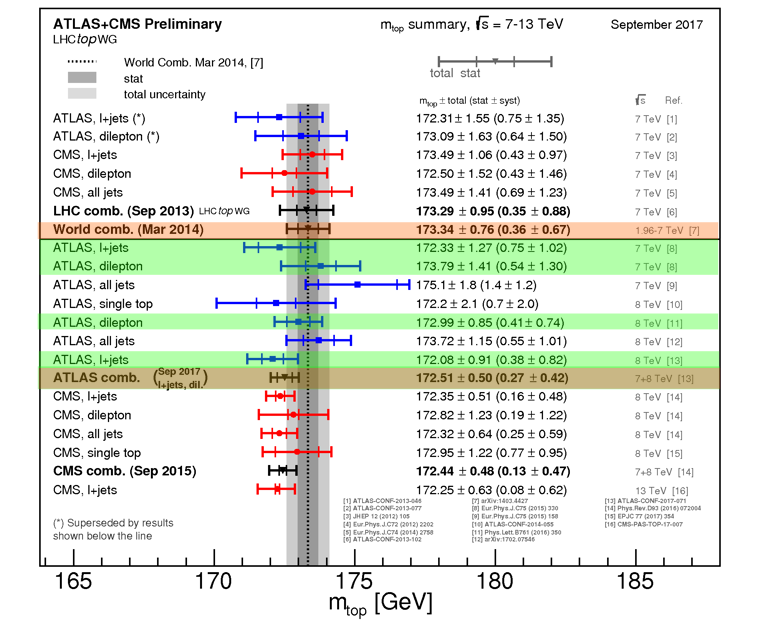
\includegraphics[width=0.9\linewidth]{Pics/mass}
	\caption{Summary of top-quark mass measurements, performed by the CMS and the ATLAS collaboration~\cite{PubR}. }
	
	\label{fig:mass}
\end{figure}




%------------------------------------------------------------------------------
\chapter{The Standard Model and the top quark}
\label{sec:SM1}
%------------------------------------------------------------------------------
In this chapter, the fundamental framework of elementary particle physics and the basic concepts are introduced. Furthermore, a more detailed  description of the top-quark is given and the interests in the top-quark mass are motivated.  

\section{Particles, forces and fields}\label{key:SM 2}
% Standard model of physics
% Author: Carsten Burgard

%%%<


\begin{figure}
	\centering



\newcommand\particle[7][white]{%
	\begin{tikzpicture}[x=1cm, y=1cm]
	\path[fill=#1,] (0.1,0) -- (0.9,0)
	arc (90:0:1mm) -- (1.0,-0.9) arc (0:-90:1mm) -- (0.1,-1.0)
	arc (-90:-180:1mm) -- (0,-0.1) arc(180:90:1mm) -- cycle;
	\ifstrempty{#7}{}{\path[]
		(0.6,0) --(0.7,0) -- (1.0,-0.3) -- (1.0,-0.4);}
	\ifstrempty{#6}{}{\path[] (0.7,0) -- (0.9,0)
		arc (90:0:1mm) -- (1.0,-0.3);}
	\ifstrempty{#5}{}{\path[] (1.0,-0.7) -- (1.0,-0.9)
		arc (0:-90:1mm) -- (0.7,-1.0);}
	\draw[\ifstrempty{#2}{dashed}{black}] (0.1,0) -- (0.9,0)
	arc (90:0:1mm) -- (1.0,-0.9) arc (0:-90:1mm) -- (0.1,-1.0)
	arc (-90:-180:1mm) -- (0,-0.1) arc(180:90:1mm) -- cycle;
	\ifstrempty{#7}{}{\node at(0.825,-0.175) [rotate=-45,scale=0.2] {#7};}
	\ifstrempty{#6}{}{\node at(0.9,-0.1)  [nosep,scale=0.17] {#6};}
	\ifstrempty{#5}{}{\node at(0.9,-0.9)  [nosep,scale=0.2] {#5};}
	\ifstrempty{#4}{}{\node at(0.1,-0.1)  [nosep,anchor=west,scale=0.25]{#4};}
	\ifstrempty{#3}{}{\node at(0.1,-0.85) [nosep,anchor=west,scale=0.3] {#3};}
	\ifstrempty{#2}{}{\node at(0.1,-0.5)  [nosep,anchor=west,scale=1.5] {#2};}
	\end{tikzpicture}
}


	\begin{tikzpicture}[x=2cm, y=2cm]
	%\draw (-0.5,0.5) rectangle (4.4, -1.5);
	%\draw (-0.6,0.6) rectangle (5.0,-2.5);
	%\draw (-0.7,0.7) rectangle (5.6,-3.5);
	
	\node at(0, 0)   {\particle[blue!20!white]
		{$u$}        {up}       {$2.3$ MeV}{1/2}{$2/3$}{R/G/B}};
	\node at(0,-1)   {\particle[blue!20!white]
		{$d$}        {down}    {$4.8$ MeV}{1/2}{$-1/3$}{R/G/B}};
	\node at(0,-2)   {\particle[blue!20!white]
		{$e$}        {electron}       {$511$ keV}{1/2}{$-1$}{}};
	\node at(0,-3)   {\particle[blue!20!white]
		{$\nu_e$}    {$e$ neutrino}         {$<2$ eV}{1/2}{}{}};
	\node at(1, 0)   {\particle
		{$c$}        {charm}   {$1.28$ GeV}{1/2}{$2/3$}{R/G/B}};
	\node at(1,-1)   {\particle 
		{$s$}        {strange}  {$95$ MeV}{1/2}{$-1/3$}{R/G/B}};
	\node at(1,-2)   {\particle
		{$\mu$}      {muon}         {$105.7$ MeV}{1/2}{$-1$}{}};
	\node at(1,-3)   {\particle
		{$\nu_\mu$}  {$\mu$ neutrino}    {$<190$ keV}{1/2}{}{}};
	\node at(2, 0)   {\particle
		{$t$}        {top}    {$173.2$ GeV}{1/2}{$2/3$}{R/G/B}};
	\node at(2,-1)   {\particle
		{$b$}        {bottom}  {$4.7$ GeV}{1/2}{$-1/3$}{R/G/B}};
	\node at(2,-2)   {\particle
		{$\tau$}     {tau}          {$1.777$ GeV}{1/2}{$-1$}{}};
	\node at(2,-3)   {\particle
		{$\nu_\tau$} {$\tau$ neutrino}  {$<18.2$ MeV}{1/2}{}{}};
	\node at(3,-3)   {\particle[green!20!white]
		{$W^{\hspace{-.3ex}\scalebox{.5}{$\pm$}}$}
		{}              {$80.4$ GeV}{1}{$\pm1$}{}};
	\node at(4,-3)   {\particle[green!20!white]
		{$Z$}        {}                    {$91.2$ GeV}{1}{}{}};
	\node at(3.5,-2) {\particle[yellow!50!white!]
		{$\gamma$}   {photon}                        {}{1}{}{}};
	\node at(3.5,-1) {\particle[pink!50!white]
		{$g$}        {gluon}                    {}{1}{}{color}};
	\node at(5,0)    {\particle[gray!50!white]
		{$H$}        {Higgs}              {$125.1$ GeV}{0}{}{}};
%	\node at(6.1,-3) {\particle
%		{}           {graviton}                       {}{}{}{}};
	
	%\node at(4.25,-0.5) [force]      {strong force (color)};
	%\node at(4.85,-1.5) [force]    {electromagnetic force (charge)};
	%\node at(5.45,-2.4) [force] {weak nuclear force (weak isospin)};
	%\node at(6.75,-2.5) [force]        {gravitational force (mass)};
	
	\draw [<-] (2.5,0.3)   -- (2.7,0.3)          node [legend] {charge};
	\draw [<-] (2.5,0.15)  -- (2.7,0.15)         node [legend] {colors};
	\draw [<-] (2.05,0.25) -- (2.3,0) -- (2.7,0) node [legend]   {mass};
	\draw [<-] (2.5,-0.3)  -- (2.7,-0.3)         node [legend]   {spin};
	
	\draw [mbrace] (-0.8,0.5)  -- (-0.8,-1.5)
	node[leftlabel] {quarks};
	\draw [mbrace] (-0.8,-1.5) -- (-0.8,-3.5)
	node[leftlabel] { leptons};
	\draw [mbrace] (-0.5,-3.6) -- (2.5,-3.6)
	node[bottomlabel]
	{ fermions\\};
	\draw [mbrace] (2.5,-3.6) -- (4.5,-3.6)
	node[bottomlabel] {gauge bosons\\};
	
%	\draw [brace] (-0.5,.8) -- (0.5,.8) node[toplabel]         {stable };
	%\draw [brace] (0.5,.8)  -- (2.5,.8) node[toplabel]         {unstable };
	%\draw [brace] (2.5,.8)  -- (4.5,.8) node[toplabel]          {force carriers};
	\draw [brace] (4.5,.8)  -- (5.5,.8) node[toplabel]       {goldstone\\bosons };
	%\draw [brace] (5.5,.8)  -- (7,.8)   node[toplabel] {outside\\standard %model};
	
	\node at (0,.8)   [generation] {1\tiny st};
	\node at (1,.8)   [generation] {2\tiny nd};
	\node at (2,.8)   [generation] {3\tiny rd};
	\node at (2.8,.8) [generation] {\tiny generation};
	
	
	\end{tikzpicture}

	\caption{Graphical } \label{fig:SM}
\end{figure}


  
%%% Local Variables: 
%%% mode: latex
%%% TeX-master: "../mythesis"
%%% End: 

\clearpage


On the most elementary scale, all known fundamental matter can be described by the Standard Model of Particle Physics (SM)~\cite{Glashow:1961tr,Glashow:1970gm,Gross:1973ju,Politzer:1973fx,Politzer:1974fr,Salam:1964ry,Weinberg:1967tq}. This fundamental mathematical framework is a combined relativistic Quantum Field Theory (QFT), which describes the interaction of all known elementary particles by the fundamental forces, gravity excluded.
In this theory the particles are represented by fields $\Psi$ ($\bar{\Psi}$  corresponds to the antiparticle). The evolution of these fields is given by the Euler-Lagrange equations, which can be determined by Hamilton's principle of stationary action $\delta S[\mathscr{L}] \!= 0 $, where $S[\mathscr{L}] $ denotes the action functional, which depends on the Lagrangian density $\mathscr{L} $. Claiming the invariance of
$\mathscr{L}$ under local gauge transformations, leads to the introduction of a  vector boson set as force mediators.

 In summary there are currently, as displayed in~\cref{fig:SM}, three generations of fermions (spin-1/2), distinguishable into quarks and leptons. Each generation consists of an up- and a down-type quark, a charged lepton and a corresponding light neutrino. While the charged leptons carry exactly one unit of elementary charge $e$, the quarks have  a irrational number of the electromagnetic charge. Furthermore, the quarks also carry the so-called colour charge, which is related to the strong interaction. The fermion generations are ordered by the increasing mass values.
In addition, there are thirteen bosonic particles in the SM, twelve vector bosons (spin-1) and one scalar goldstone boson (spin-0).
 The charged $W^{\pm}$-boson and the two uncharged vector bosons, the $Z^0$-boson and the photon $ \gamma$, are the participants in electroweak (EW) processes, while the strong force interacts via eight massless gluon fields $g$. The scalar Higgs boson is the latest discovered particle of the Standard Model and represents the mass generating mechanism of the particles in the SM framework. An overview of the most important properties of all SM particles is shown in~\cref{tab:T21}. 
 
 The  mass values of the quarks and the charged leptons are significant, compared to the neutrino masses, where only lower limits could be established so far.
 \begin{center}
\captionof{table}{ Summary of important properties of the SM particle content. The upper part displays the current mass value $m_i$  for the different fermion generations ($i = I, II, III$), the electromagnetic charge $Q$ in units of the elementary charge $e$ and the third component of the weak isospin $I_3$. The mass values for the gauge and goldstone bosons are shown below, together with the spin, the electromagnetic charge and the colour charge of the strong interaction. All values refer to 2017 and are taken from~\cite{Olive:2016xmw}. }\label{tab:T21}

	
\vspace{0.3cm}	
	

\begin{tabular}{>{\centering}m{1cm} >{\centering}m{2.6cm} >{\centering}m{0.5cm} >{\centering}m{2.3cm} >{\centering}m{0.8cm}  >{\centering}m{2.5cm} >{\centering}m{0.1cm} >{\centering}m{1cm}>{\centreing}m{0.7cm}} \toprule
%\emph{ }&		&	\emph{}&		\emph{fermions}&		\emph{} & & &\\  
%\midrule
				 		Fermions							&	m$_I$ / [MeV]                &          		          &	m$_{II}$ / [MeV]                       &	                                      &	m$_{III}$ / [MeV]                   &       &  Q / [e]    &    I$_3$  &                      
							 										\midrule
			\begin{center}				 	\begin{pmatrix} $u$ \\ $$d \end{pmatrix}  \end{center}    &    \begin{tabular}{1} \small 2.2^{+~0.6}_{-~0.4} & \small 4.7^{+~0.5}_{-~0.4}  \end{tabular} &   	\begin{pmatrix} $c$ \\ $s$ \end{pmatrix} &  \begin{tabular}{1}\small 1.27(0.03)\cdot~10^3 & \small 96^{+~8}_{-~4}   \end{tabular} & \begin{pmatrix} $t$ \\ $b$ \end{pmatrix}  &  \begin{tabular}{1} \small 173.1(0.6)\cdot~10^3  & \small 4.18^{+~0.04}_{-~0.03}~\cdot 10^3  \end{tabular} & &\begin{tabular}{1}+2/3 & -1/3 \end{tabular} & \begin{tabular}{1}+1/2 & -1/2 \end{tabular}   &
			\begin{center}				 	\begin{pmatrix} $e$ \\ $\nu_e$ \end{pmatrix}  \end{center}    &    \begin{tabular}{1} \small 0.5109989461(31) & \small<~2\cdot10^{-6} \end{tabular} &   	\begin{pmatrix} $\mu$ \\ $\nu_{\mu}$\end{pmatrix} &  \begin{tabular}{1}\small 105.6583745(24) &\small <~0.19\cdot10^{-6}~\end{tabular} & \begin{pmatrix} $\tau$ \\ $\nu_{\tau}$ \end{pmatrix}  &  \begin{tabular}{1} \small 1776.86(0.12) & \small <~18.2\cdot10^{-6} \end{tabular} & \begin{tabular}{1}  &  \end{tabular} & \begin{tabular}{1}-1 & 0 \end{tabular}  & \begin{tabular}{1} -1/2 &+1/2 \end{tabular}  &
%							 &  	\begin{pmatrix} e \\ $\nu_e$ \end{pmatrix}    &    \begin{tabular}{1} masse & mass \end{tabular} &   	\begin{pmatrix} u \\ d \end{pmatrix} &  \begin{tabular}{1} masse & mass \end{tabular} & \begin{pmatrix} u \\ d \end{pmatrix}  &  \begin{tabular}{1} masse & mass \end{tabular} & \begin{tabular}{1} masse & mass \end{tabular} & \begin{tabular}{1} masse & mass \end{tabular}  &\\
\midrule
 Bosons & & &m / [MeV]&  &Spin& & Q / [e]&Colour&
\midrule
W^{\pm} & & & 80.385(0.015)\cdot 10^3& &1 & & $\pm$1&no&
Z^0 & & & 91.1876(0.0021)\cdot 10^3 & & 1& & 0& no&
$\gamma $ &  & &< 1\cdot 10^{-24}& &1 & & 0 & no&
$g$ &  & & 0& & 1& &0 & yes&
$H^0$ &  & & 125.09(0.24)\cdot 10^3& &0& & 0 &no &








\bottomrule
\end{tabular}

\end{center}

\vspace{0.1cm}




 


 
\section{Fundamental forces and symmetry breaking}
In terms of a field theory, the SM basically combines Quantum Chromo Dynamics (QCD), the theory of the strong interaction, and the unified electroweak theory (EW). Both theories can be identified with a symmetry group.
The fundamental concept of the  elementary interactions rests on the idea, that the interactions can be mathematically expressed by  local gauge transformations:
\begin{equation}\label{trafo}
\Psi \longrightarrow \Psi'(x) =  e^{i\alpha(x)}\Psi(x).
\end{equation}  
This is the most general from of a finite local transformation with a phase factor $\alpha(x)$, whose specific functional form depends  on the chosen symmetry group. 
The cornerstone of the SM concept is that the corresponding Lagrangian densities are invariant under the local gauge transformations.  
In order to achieve this invariance, covariant derivatives  and the above mentioned vector gauge fields are introduced. Nevertheless, the fact that the gauge bosons are massive, violates the locale gauge invariance. This contradiction can be solved by the concept of spontaneous symmetry breaking, bringing up the famous Higgs boson.

 Coming up next is a short introduction of QCD and the electroweak theory before a brief approach is taken to clarify the concept of symmetry breaking. This short introduction is based on the work of W. Hollik~\cite{Hollik:2010id}. 

\subsection{Quantum Chromo Dynamics}\label{QCD}
The interaction of massive spin-1/2 quarks and massless spin-1 gluons is described by the non-abelian gauge group $SU(3)_C$, where $C$  refers to the charge of the strong interaction, called colour. The corresponding Lagrangian density is given by
\begin{equation}\label{LQCD}
\mathscr{L}_{QCD} = - \frac{1}{4} F^a_{\mu\nu}F^{\mu\nu}_a +\sum_{f}\bar{\Psi}_f^C(i\gamma^{ \mu}D_{\mu}-m_f)\Psi_f^C, \hspace{0.5cm}\text{with}
\end{equation}
\begin{equation}\label{Fieldtensor}
F^a_{\mu\nu} = \partial_{\nu}G_{\mu}^a - \partial_{\mu}G_{\nu}^a+g_sf^{abc}G_{\mu}^bG_{\nu}^c.
\end{equation}
In the first term $F^a_{\mu\nu}$  is the field strength tensor, derived from eight massless gluon fields $G_{\mu}^a$. $\partial_{\nu}$ denotes the derivative of the four-vectors\footnote{$\partial_{\nu}$ =($\partial_{t}$, $\partial_{1}$, $\partial_{2}$, $\partial_{3}$).}. The interaction strength is determined by the strong coupling constant $g_s$.  $f^{abc}$ are the structure constants of the strong interaction, with the indices $a,b,c$ running over all eight degrees of freedom of the $SU(3)_C$ group. The number of degrees of freedom results from the eight generators $T^a$ of the $SU(3)_C$  group in its fundamental representation, which can be expressed by the Gell-Mann matrices, $T^a=\lambda^a/2$, with the Lie-algebra:
 \begin{equation}
[T^a,T^b]=if^{abc}T^c.
\end{equation}
 The last term of the Lagrangian sums over all quark flavours ($f= u,d,...$), with the quark fields $\Psi_f^C$ and masses $m_\text{f}$\footnote{These mass terms break the weak isospin and hypercharge symmetry. The mass generation mechanism to solve these problems will be introduced in \cref{Higgsm}. }. The quarks are grouped to $SU(3)_C$ colour triplets ($C$ = red, green, blue), while the corresponding antiquarks belong to the conjugated fundamental $SU(3)_C$ representation and carrying matching anticolours. In contradiction to the photon, the force carrier of the electromagnetic force, the gluons themselves are carrying the colour charge, which results in gluon-gluon self-coupling. 
In order to keep the  QCD-Lagrangian invariant under local $SU(3)_C$ gauge transformations, the covariant derivative 
\begin{equation}\label{Kovariant}
D_{\mu}=\partial_{\mu}+ig_sT^aG_{\mu}^a,
\end{equation} 
is introduced.

\noindent The QCD-coupling strength can be further characterized by  $\alpha_s = g_s^2/4\pi$, which depends  on the energy scale and therefore can not be treated as constant. Furthermore, to compensate ultraviolet divergences, a renormalization with a specific reference scale $\mu(Q^2)$ has to be made. A convenient choice is the renormalization to the $Z^0$-boson mass with a measured coupling of $\alpha_s(Q^2=M_Z^2) = 0.1184 \pm 0.0031$~\cite{Bethke:2000ai}. In addition, for short distances (= high energies) the strength of the strong coupling becomes sufficiently small and one observes free particle like behaviour, which is known as asymptotic freedom. On the other hand, in the low energy regime (= long distances), the coupling is differently and can be expressed by 
\begin{equation}\label{alphas}
\alpha_s(Q^2)=\frac{12\pi}{(33-2N_f)~\text{ln}(\frac{Q^2}{\Lambda_{QCD}^2})},
\end{equation}
where $N_f$ refers to the number of participating quark flavours at the energy $Q^2$. $\Lambda_{QCD}$ is of the order $O(200~\text{MeV})$ and represents the energy scale where the perturbation theory  breaks down, due to the ultraviolet divergences. As ~\cref{alphas} suggests, the coupling strength increases with decreasing energy, resulting in the confinement of the quarks. Consequently, quarks and gluons do not propagate over macroscopic distances and can therefore only be observed via the hadrons -the colour neutral quark bound states- which are experimentally accessible. One general refers this as confinement, where the hadrons represent the singlet states of  the $SU(3)_C$-group and are either baryons, consisting of three quarks or antiquarks,  or mesons which are a quark-antiquark pairs. 
























\subsection{The electroweak force}\label{EW}
The electromagnetic force, described by Quantum Electrodynamics QED, and the weak interaction are unified by the theory of Glashow, Weinberg and Salam (GSW)~\cite{Glashow:1961tr,Weinberg:1967tq,Salam:1964ry}, which is based on the $SU(2)_L\times U(1)_Y$ symmetry group product. The invariance requirement of the corresponding Lagrangian density leads to the introduction of the four well known physical vector gauge bosons $W^{\pm}, Z^0$ and $\gamma$.

In the framework of the weak interaction, with its fundamental representation expressed by the $SU(2)$ group, the fermions are grouped in left-handed doublets and right-handed singlets of the weak isospin $I_3$
\footnote{The term handedness refers to the fact that the fields can be split into a right-handed and left-handed part, which are defined by the eigenvalues of the projection operator $P_{L/R}= \frac{(1\pm \gamma^5)}{2}$ with the Dirac matrix $\gamma^5$.}. 
A striking observation is the maximal violation of the parity conservation by weak interaction processes.\footnote{The sign changing transformation of space coordinate $\vec{r}$ is called parity. }
Consequently only left-handed fermions and right-handed antifermions contribute in weak interaction processes.  Furthermore, the  quark mass eigenstates ($d,s,b$), which couple to the gauge fields, are not identical with the weak isospin eigenstates of the quarks ($d',s',b'$). These different states are connected by the  Cabbibo-Kabayashi-Maskawa (CKM) matrix \cite{Cabibbo:1963yz, Kobayashi:1973fv}:
\begin{equation}\label{CKM}
\begin{pmatrix}
d'\\
s'\\
b'
\end{pmatrix}
=
 \begin{pmatrix}
\rm  V_{ud} &\rm V_{us} &\rm V_{ub}\\
\rm  V_{cd} &\rm V_{cs} &\rm V_{cb}\\
\rm  V_{td} &\rm V_{ts} &\rm V_{tb}
\end{pmatrix} 
\cdot
\begin{pmatrix}
d\\
s\\
b
\end{pmatrix}.
\end{equation}
The CKM matrix elements can only be determined by experimental measurements~\cite{Olive:2016xmw}. The diagonal elements are measured close to unity.  Following from the quark flavour mixing in the weak interaction, one can observe quark flavour oscillations and the violation of the CP\footnote{CP represents the product of charge conjugation and parity.} conservation.

Compared to the weak interaction, QED does not distinguish between the left and right handed particles. In the GSW model, electromagnetic interactions are taken into account by the $U(1)$ symmetry group, where the weak hypercharge $Y$ is added as an additional quantum number connected to the electromagnetic charge $Q$ and the weak isospin $I_3$ via the Gell-Mann–Nishijima formula:
\begin{equation}
Q = I_3 + \frac{Y}{2}.
\end{equation}

 The unified electroweak theory is described by  $SU(2)_L\times U(1)_Y$  and has the four group generators $I_a$ with $a$ = 1,2,3 and $Y$, with the Lie-algebra:
\begin{equation}
[I_a,I_b]=i\epsilon_{abc}I_c  \hspace{1.0cm} \text{and} \hspace{1.0cm} [I_a,Y]= 0.
\end{equation}
$\epsilon^{abc}$ denotes the Levi-Civita symbol with the indices running over the triplet ($a,b,c = 1,2,3$).
 The corresponding  Lagrangian for the unified electroweak interaction theory takes the following functional from:
\begin{equation}\label{LGSW}
 \mathscr{L}_{GSW} = -\frac{1}{4} F^a_{\mu\nu}F^{\mu\nu}_a -\frac{1}{4} f_{\mu\nu}f^{\mu\nu}  +\sum_{f}\bar{\Psi}_{f_R}(i\gamma^{ \mu}D_{\mu_R})\Psi_{f_R}  +\sum_{f}\bar{\chi}_{f_L}(i\gamma^{ \mu}D_{\mu_L})\chi_{f_L}.
\end{equation}

 In order to keep the Lagrangian gauge invariant, four gauge vector fields are introduced, a boson triplet $\vec{W} = (W_1,W_2,W_3)^T$ and a boson singlet $B_0$. The field strength tensors of the GSW-Model, which describe the kinematics of the fields, are:   

 \begin{equation}\label{FieldtensorW}
 F^a_{\mu\nu} = \partial_{\nu}W_{\mu}^a - \partial_{\mu}W_{\nu}^a+g\epsilon^{abc}W_{\mu}^bW_{\nu}^c,
 \end{equation}
 \begin{equation}\label{FieldtensorB}
 f_{\mu\nu} = \partial_{\nu}B_{\mu}- \partial_{\mu}B_{\nu}.
 \end{equation}

 Fermion interactions are taken into account with the last terms of the  $\mathscr{L}_{GSW} $. The fileds $\Psi_{f_R}$ describe the interaction of the right-handed fermion singlets, while the ${\chi}_{f_L}$ fields take care of the left-handed fermion doublets. Furthermore, two different covariant derivatives are introduced with respect to the orientations of the fermions. Left-handed charged fermions take part in weak- and electromagnetic processes, which leads to:    
\begin{equation}\label{Kovariant2}
D_{\mu_L}=\partial_{\mu}+ig'\frac{Y_L}{2}B_{\mu} + ig\vec{I}\cdot \vec{W_{\mu}}.
\end{equation}
All four gauge fields  keep the required invariance under the corresponding gauge transformations. The coupling strength of the interactions is given by the constants $g$ and $g'$. In contrast to the left-handed fermions, the covariant derivative takes a much simpler from for right-handed fermions:
\begin{equation}\label{Kovariant1}
D_{\mu_R}=\partial_{\mu}+g'\frac{Y_R}{2}B_{\mu}.
\end{equation} 

The four vector fields, appearing in gauge theory, can easily be related to the physical quantities which have been studied extensively. 
The observed $W$-bosons, mediating the charged current (CC), are given by the combination
\begin{equation}\label{EWtrafo1}
 W^{\pm}_\mu = \frac{1}{2}(W^{1}_\mu\pm iW^{2}_\mu),
\end{equation}
of the two gauge fields $W^{1}_\mu$ and $W^{2}_\mu$. The $Z^0$-boson and $\gamma$ (represented in QED as $A_\mu$) are mediating the neutral current (NC) and can be constructed from the two gauge fields $B_{\mu}$ and $W_{\mu}^{0}$ by an orthogonal rotation:
\begin{equation}\label{EWtrafo2}
\begin{pmatrix}
A_\mu\\
Z^0_\mu
\end{pmatrix}
=
\begin{pmatrix}
cos\Theta_W & sin\Theta_ W \\
-sin\Theta_W & cos\Theta_W  \\

\end{pmatrix}
\cdot 
\begin{pmatrix}
B_\mu\\
W^0_\mu
\end{pmatrix},
\end{equation}
 $\Theta_W$ is the Weinberg angle, which relates the two coupling constants $g$ and $g'$ with the weak hypercharge $Y_L$:
\begin{equation}\label{Weinber2}
cos \Theta_W = \frac{g}{\sqrt{g^2+g'Y^2_L}}.
\end{equation} 

The experimentally observed neutral vector bosons can be expressed in terms of the gauge fields and the coupling constants: 

\begin{equation}
A_\mu = \frac{gB_\mu -g'Y_LW_\mu^0}{\sqrt{g^2+g'Y^2_L}} ~~~~\mathrm{and} ~~~~Z_\mu^0 = \frac{gW_\mu^0 +g'Y_LB_\mu}{\sqrt{g^2+g'Y^2_L}}.
\end{equation}

The GSW-Model shows in a very elegant way the unification of two interactions, by introducing just a minimal set of gauge fields. Nevertheless, this theory is not able to deal with massive gauge bosons, because mass terms inside the Lagrangian would break its gauge symmetry. However, since measurements have shown that the $W^\pm$ and the $Z^0$-boson are in fact very massive objects, the implementation of a mass generation mechanism has been a cornerstone of research in elementary particle physics over the past decades.

 In following sections of this thesis, the gauge fields ($W^\pm$, $Z^0$) are just denoted by $W$ and $Z$.



 
\subsection{The Higgs mechanism}\label{Higgsm}
\begin{figure}[h]
	\centering
	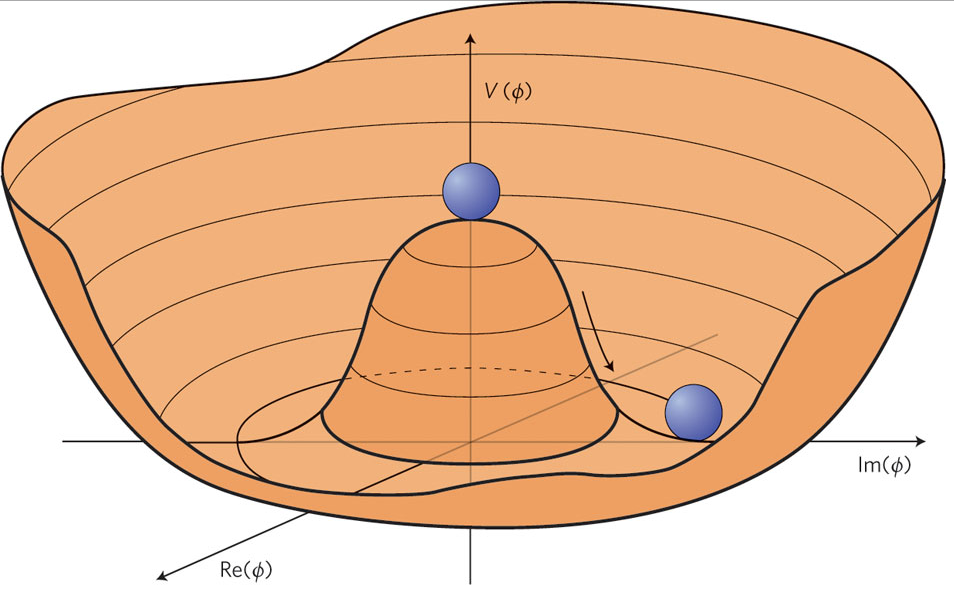
\includegraphics[width=0.4\linewidth]{Pics/cp1/Higgs}
	\caption{Illustration of the Higgs potential for $\mu^2>0 $ and $\lambda>0$ from ~\cite{Ellis:2013jnq}. The complete set of vacuum states is given by the circular potential minimum. Excitations in the transversal direction lead to the introduction of a massive spin-0 particle, the Higgs boson.}
	
	\label{fig:Higgs}
\end{figure}

The non-vanishing masses of the electroweak gauge bosons, one of the biggest issues inside the SM framework, has been solved by Brout, Englert, Guralnik, Hagen, Kibble and Higgs~\cite{Higgs:1964ia,Higgs:1964pj,Guralnik:1964eu,Englert:1964et}, by the introduction of an additional complex scalar field - the so-called Higgs field- as a weak isospin $I_3$ doublet
\begin{equation}
\Phi(x) =
 \begin{pmatrix}
	\phi^{\dagger}(x)\\
	\phi_0(x)
\end{pmatrix},
\end{equation} 
  with the hypercharge $Y$=1. The coupling of $\Phi$ to the electroweak gauge fields is realized by adding
  \begin{equation}\label{Lhiggs}
  \mathscr{L}_{Higgs} = (D_{\mu}\Phi )^{\dagger}(D^{\mu}\Phi)-V(\Phi,\Phi^{\dagger}).
  \end{equation}
  to the total Lagrangian of the Standard Model.
  The covariant derivatives $D_{\mu}$ are introduced in~\cref{Kovariant2} and include the coupling to the electroweak gauge fields $\vec{W}_{\mu}$ and $B_{\mu}$.
  In addition the potential  
  \begin{equation}\label{HiggsV}
  V(\Phi,\Phi^{\dagger}) = -\mu^2\Phi^{\dagger}\Phi + \frac{\lambda}{4}(\Phi^{\dagger}\Phi)^2, 
  \end{equation}
  with the two real constants $\mu^2$ and $\lambda$ is added.  This so-called Higgs potential
  is symmetric under rotations around the z-axis and contains the self interaction of the Higgs field. Its characteristic shape (see~\cref{fig:Higgs}) is determined by choosing $\mu^2>0 $ and $\lambda>0$. In the vacuum ground state, the potential has a minimum at a non-zero value $\Phi\neq$0. Furthermore,  $V(\Phi,\Phi^{\dagger})$ takes its minimum value in the complex plane w.l.o.g. for all field configurations satisfying~$\Phi^{\dagger}\Phi=2\mu^2/\lambda$. By constraining the field configuration to be real and free of electrical charge, one gets for  the vacuum expectation value:
\begin{equation}
\langle\Phi_0\rangle = \frac{1}{\sqrt{2}}
\begin{pmatrix}
0\\
\nu
\end{pmatrix}
, \text{ \hspace{0.5cm} with}~ \nu = \frac{2\mu}{\sqrt{\lambda}}.
\end{equation}


 In general $\mathscr{L}_{Higgs}$ has the $SU(2)_L\times U(1)_Y$ symmetry of the electroweak gauge theory. However, this is not the case for the groundstate $\langle\Phi\rangle _0$ of the system, which contains only the gauge symmetry of the electromagnetic force $U(1)_Y$. Thus the  actual symmetry of the Lagrangian is  broken, which is known as \textbf{spontaneous symmetry breaking}.


Deviations of the Higgs potential from its groundstate,  like $\phi_0(x)=\nu + H(x)+ i\chi(x)$, allow to express the potential in the following from:
\begin{equation}
  V(\Phi,\Phi^{\dagger})=\mu^2H^2+\frac{\mu^2}{\nu}H^3 + \frac{\mu^2}{4\nu^2}H^4.
\end{equation}
The contributions from $\chi(x)$ and $\phi^{\dagger}$ are massless unphysical degrees of freedom and can be eliminated by choosing an appropriate gauge transformation. $H$ leads to the introduction of a scalar particle (the Higgs boson) with a mass of
$m_{\text{H}}=\sqrt{2}\mu$
and self coupling vertices of the Higgs field.

The coupling of the gauge fields $\vec{W}_{\mu}$ and $B_{\mu}$ and the Higgs field arises from the  kinetic term of the Lagrangian~\cref{Lhiggs}. With the transformations~\cref{EWtrafo1,EWtrafo2}, the masses of the observed bosons are:
\begin{equation}
 m_W=\frac{1}{2}g\nu ~~~~ \mathrm{and} ~~~~m_Z=\frac{1}{2}\sqrt{g^2+g'^2}\nu. 
\end{equation}  
 
 
 The Higgs mechanism is also able to explain the observation of massive charged fermions by Yukawa coupling between the Higgs field and the charged fermion fields.
This can be expressed with the additional term:  
\begin{equation}
\mathscr{L}_{Yukawa}=\sum_{f}m_f(\bar{\Psi}_f\Psi_f-\bar{\Psi}_f\Psi_f H).
\end{equation} 

In this formula, the sum runs over the massive fermions, represented by the fields $\Psi_f$ and $\bar{\Psi}_f$. The fermion mass terms are related to the Yukawa coupling via individual coupling constants $G_f$, which are proportional to the fermion masses: 
\begin{equation}\label{Higpro}
G_f = \frac{\sqrt{2}}{\nu} m_f.
\end{equation} 

The Standard Model is not able to predict the mass of the Higgs boson $m_H$, as well as the different Yukawa coupling constants (or the fermion masses), which therefore have to be determined by measurements. The discovery of the Higgs boson in the year 2012 by the ATLAS and CMS collaborations~\cite{Aad:2012tfa,Chatrchyan:2012xdj}, was the fist evidence  for the Higgs mechanism and has been a milestone for the Standard Model. Currently the Higgs boson and its properties are the subject of intense studies at the LHC experiments. 
























\section{Relevance of the top quark}\label{Relevanz}

The first experimental evidence of top quarks from the CDF~\cite{Abe:1995hr} and the $D \emptyset$~\cite{Abachi:1995iq} collaborations in 1995, was a tremendous success in the field of particle physics. 
The production of top-quarks was observed in proton-antiproton collisions at a center-of-mass energy of 1.8~TeV. The existence of top quarks was already predicted 1977, as the weak isospin partner of the bottom quark~\cite{Herb:1977ek}. 

The top quark contributes noticeably to higher-order (HO) corrections e.g. in perturbation scattering theory.  From an experimental point of view, these HO corrections offer the possibility to perform observations at energy scales even higher than the center-of-mass energy of the actual experiment. Therefore, indirect particle searches can be performed by testing particle properties without directly observing them. This unique feature was used, together with precision measurements at the $e^+e^-$-collider LEP\footnote{Large Electron-Positron Collider.}, to constrain the top-quark mass to a range of 173$^{+18}_{-20}$~GeV.~\cite{LEPEW:1994aa}
\begin{figure}[h]
	\centering
	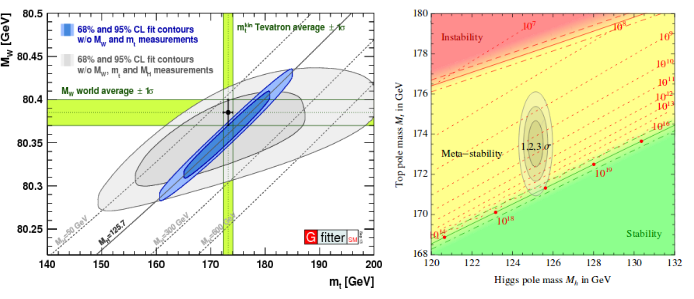
\includegraphics[width=0.9\linewidth]{Pics/Relevanz}
	\caption{Left: electroweak fit of the SM from ~\cite{Baak:2012kk}. $m_{\text{W}}$ is displayed vs $m_{\text{top}}$ with the direct measurements marked green. The  counters show the fit results for the indirect measurements of both masses, with the measured $m_{\text{H}}$ excluded (grey) and fixed (blue).
		Right: phase diagram of the EW vacuum in the $m_{\text{H}}-m_{\text{top}}$ plane from~\cite{Buttazzo:2013uya}. The plane is divided into regions of absolute stability, meta-stability and instability. The grey contour represents the area under experimental investigation.}
	\label{fig:Relevanz}
\end{figure}

With the discovery of the Higgs boson and the measurement of its mass $m_{\text{H}}$, all fundamental parameters of the SM are known and have been used for testing the self-consistency of the SM by global electroweak fits, as displayed in \cref*{fig:Relevanz} (left). The contours (gray/blue) belong to the 68\% and 95\% confidence level (CL) and result from scans  over fits of the $W$-boson mass $m_{\text{W}}$ vs the top-quark mass $m_{\text{top}}$ with a fixed $m_{\text{W}}$. The green bands mark the results from direct measurements of the $m_{\text{W}}$ and $m_{\text{top}}$. 
Additionally, the dashed lines represent values for the Higgs mass ($m_{\text{H}}$) obtained from SM constrains, while the grey contours display the results of the indirect $m_{\text{W}}$ and $m_{\text{top}}$ determination, which agrees, within all uncertainties, quite well with the direct results for $m_{\text{W}}$ and $m_{\text{top}}$.
Despite the inclusion of the measured  Higgs mass (solid line), leading to a significant reduction of the obtained contour (blue contour), the results still confirm the direct observations. This is a good  example for the remarkable consistency of the SM and the important role of $m_{\text{top}}$ inside this framework.~\cite{Baak:2012kk}



Furthermore, with its unusually high mass close to the electroweak symmetry breaking scale, the top quark plays a special role in several theoretical models, e.g. in top-colour models~\cite{Hill:1991at,Hill:1994hp}, where the  gauge extension of the SM is considered in the context of dynamical electroweak symmetry breaking~\cite{Bardeen:1989ds}. 

Moreover, the top-quark mass itself might be sensitive to new physics beyond the SM (BSM). There are several BSM theories, predicting the decay of heavy unstable exotic particles into top quarks that might result into contributions, which can be observed in higher-order corrections (see for example \cite{Kong:2014jwa}).


Finally, the top-quark mass, together with the Higgs boson mass, determines the different phases of the electroweak vacuum in the SM. In~\cref{fig:Relevanz} (right), the stable, metastable and instable regions of the EW vacuum are displayed.  The most interesting experimental region of the top-quark and Higgs boson mass is marked by the grey contours for different CL levels. The dashed lines denote the uncertainties of the strong gauge coupling and the theoretical errors, while the dotted contour line displays the instability scale $\Lambda$.
The grey contours mark the region under current experimental investigation, where the vacuum state lies in a critical region between the stable and the metastable state. More precise measurements are needed, in order to further investigate this region.~\cite{Buttazzo:2013uya}



As already mentioned, the mass value of the top quark is  a fundamental parameter of the SM and therefore particularly interesting in terms of physic analyses. For this measurement, one is interested to determine $m_{\text{top}}$ from top-quark pairs. In general, there are basically two main experimental methods, which are used to determine the top-quark mass directly from the $t\bar{t}$ final state:


\begin{itemize}
	
	\item The first method is the so-called \textbf{matrix element method}, where the top-quark mass is determined by a maximum likelihood approach. An event by event probability is calculated, depending on the assumed results of the measurements, i.e. of $m_{\text{top}}$, using the leading-order matrix element. The evaluated probability defines the chances to have an $t\bar{t}$ event, with the assumed $m_{\text{top}}$ value. From these probability density functions, the likelihood and finally top-quark mass are computed.~\cite{Castro:2014cva}   
	
	\item The analysis presented here, is based on the \textbf{template method}. Monte Carlo based distributions of kinematic variables are simulated for different mass values $m_{	\text{top}}^{MC}$. These distributions are fitted to analytical functions and parametrized as probability density functions,  depending on the mass value. This allows the computation of a likelihood value and the extraction of the $m_{\text{top}}^{MC}$ value in an unbinned maximum likelihood fit.   
\end{itemize}

 Both analysis methods use the  mass concept corresponding to the MC simulated distributions. The main difficulty is the relation to  theory, since  the $m_{	\text{top}}^{MC}$ definition does not take the  renormalization into account, while this plays an  important role in the different theoretical approaches. 











   

\section{Top-quark production}
In the Standard Model, top quarks can be produced either as single particles 
(single tops) via electroweak processes or as a quark pair from strong interactions, which lead to a pair of a top and an antitop quark ($t\bar{t}$).    

\subsection{Single top-quark production}
The production of single top quarks was first observed at the Tevatron 2009~\cite{Abazov:2009ii,Aaltonen:2009jj}. There are three possible single top production channels. Their Feynman diagrams in leading-order (LO) are displayed in~\cref{fig:single}.


\begin{figure}[h]
	\centering
	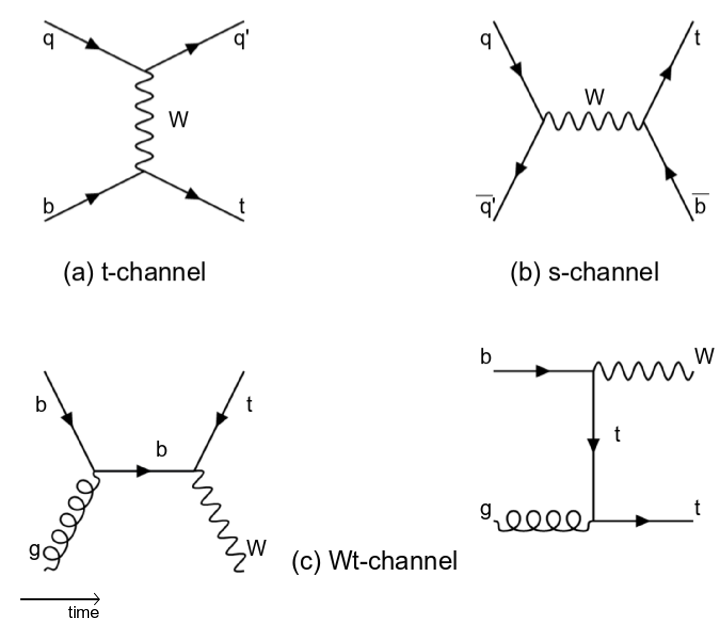
\includegraphics[width=0.5\linewidth]{Pics/cp1/single}
	\caption{Leading-order single top production pair production in three different channels s, t and Wt.} 
	\label{fig:single}
\end{figure}

 The \textbf{t-channel} process~\cref{fig:single} (a) is characterized by the transition of a bottom quark $b$ into a top quark, while a virtual $W$-boson is exchanged with a lighter quark or antiquark. This channel is the most significant contributor to the overall production.

The smallest production of single top quarks at the LHC arises from the \textbf{s-channel}~\cref{fig:single} (b). A quark and antiquark produce a virtual $W$-boson, decaying into a top and an antibottom quark (respectively into an antitop and a bottom quark).

Moreover, at the LHC, single top quarks can also be produced in the \textbf{Wt-channel}. In this channel, a $W$-boson is radiated from a bottom (anti-bottom) quark.

The  predicted production cross-sections of single-top quarks are calculated  for proton-proton collisions at a centre-of-mass energy of $\sqrt{s}=13$~TeV, for a top quark mass of 172.5~GeV, with modern theory predictions with the Hathor v2.1 program~\cite{Aliev:2010zk,Kant:2014oha}. For the evaluation of the PDF and $\alpha_{s}$ uncertainties, the following PDF sets are added in quadrature: PDF4LHC~\cite{Botje:2011sn} with the MSTW2008 68\% CL NLO~\cite{Martin:2009bu,Martin:2009iq}, CT10 NLO~\cite{Lai:2010vv} and NNPDF2.3~\cite{Ball:2012cx}. The results, with the total uncertainties, are displayed in~\cref{tab:T23}.



\begin{center}
	\captionof{table}{Combined production cross-section of single quarks + antiquarks, taken from~\cite{single}.}\label{tab:T23}
	
	
	\vspace{0.3cm}	
	
	
\begin{tabular}{>{}m{4.0cm}>{}m{4.0cm}} \toprule
		
		Process& Cross-Section/[pb] \\
		
		\midrule
		t-channel	&216.99$^{+9.04}_{-7.71}$\\
		s-channel	&10.32$^{+0.40}_{-0.36}$\\
		Wt-channel	&71.7$^{+1.80}_{-1.80}$\\
		
		\bottomrule
	\end{tabular}
	
\end{center}


\noindent At the LHC, the cross-section for single top quarks differs from the cross-section for anti-top quarks. The asymmetry of the production cross-section for $t$  and $\bar{t}$ is related to the nature of proton-proton collisions, where the only source for antiquarks is the sea quark distribution of the proton. This reduces the chance of having an antiquark in the initial state dramatically. A good example is given by the results of the cross-section measurement in the t-channel at $\sqrt{(s)}$=13~TeV~\cite{Aaboud:2016ymp}: 
\begin{equation*}
\sigma_ {t_{ch}}(tq)= 156\pm 5~(\text{stat.})\pm 27~(\text{syst.}) \pm 3~(\text{lumi}.)~\text{pb}, 
\end{equation*}
\begin{equation*}
\sigma_ {t_{ch}}(\bar{t}q)= 91\pm 4~(\text{stat.})\pm 15~(\text{syst.}) \pm 2~(\text{lumi}.)~\text{pb}.
\end{equation*}

 

.   


\subsection{Top-quark pair production}
\begin{figure}[h]
	\centering
	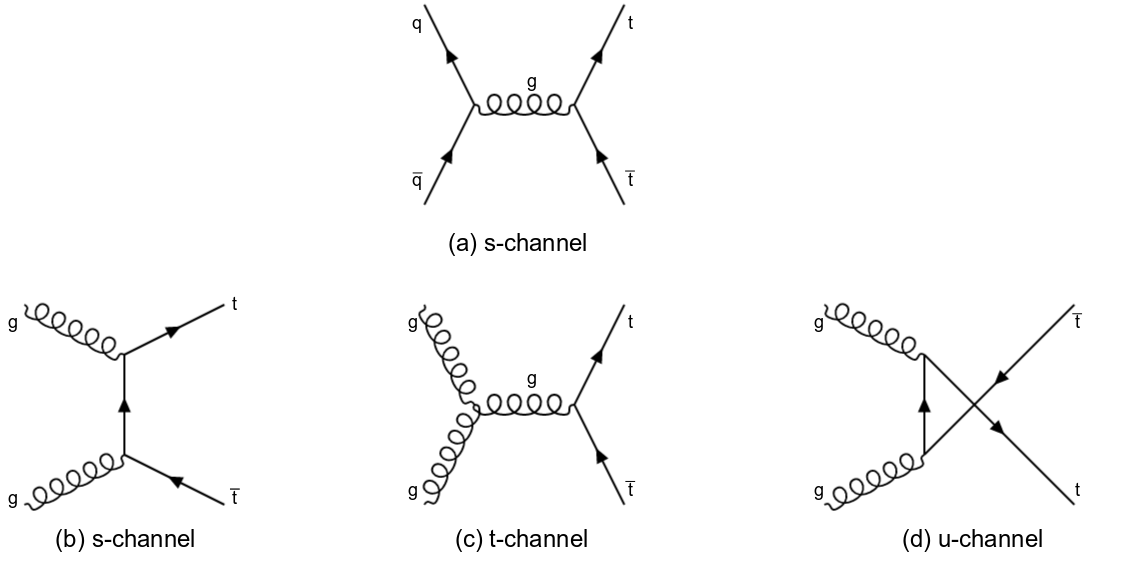
\includegraphics[width=0.70\linewidth]{Pics/cp1/ttbar}
	\caption{Leading-order top-quark pair production. Fig. (a) shows the quark- antiquark annihilation, fig. (b)-(d)  the gluon-gluon fusion.} 
	\label{fig:ttbar}
\end{figure}




\noindent The $t\bar{t}$-production processes can be distinguished into gluon-gluon fusion ($gg\rightarrow t\bar{t}$) and quark-antiquark annihilation ($q\bar{q}\rightarrow t\bar{t}$), which are both displayed in~\cref{fig:ttbar} in LO. At the LHC, the $t\bar{t}$-production is dominated by the gluon-gluon fusion ($\approx$ 90~\%). 
This issue has two reasons. One reason can be seen by considering the corresponding momentum fractions $x$ necessary to produce a top-quark pair at the LHC, which can be estimated under the assumption $x_i \approx x_j$:
\begin{equation}
x \geq 2m_{	\text{top}}/\sqrt{s}.
\end{equation}
With a center-of-mass energy of 13~TeV and an approximated top-quark mass of 173~GeV, this leads to $x \approx 0.027$. This low $x$ regime is, as shown by~\cref{fig:PDF}, highly dominated by the gluon PDF, which explains the strong gluon fusion contributions of the  $t\bar{t}$-production at LHC. 
 Furthermore, the only source for antiquarks are the sea distributions of the protons, while quarks are also present in the valence distributions. Therefore, the chances of interactions with antiquarks are slightly reduced. 
 
 
\noindent With modern theory predictions~\cite{Cacciari:2011hy,Beneke:2011mq,Baernreuther:2012ws,Czakon:2012zr,Czakon:2013goa} the $t\bar{t}$ production cross-section can be calculated with the Top++2.0 program~\cite{Czakon:2011xx}. For these calculations, the top-quark mass is assumed to be 172.5 GeV. 
 The predictions are computed with the corresponding scale (first term), PDF and $\alpha_s$ uncertainties (second term). For the latter one,  PDF4LHC~\cite{Botje:2011sn} with  MSTW2008 68\% CL NLO~\cite{Martin:2009bu,Martin:2009iq} are used,  as well as the CT10 NNLO~\cite{Gao:2013xoa} and NNPDF2.3~\cite{Ball:2012cx} PDFs. Furthermore, there is a mass uncertainty included (third term). For a center-of-mass energy of  13~TeV, top-quark pair production cross-section  is obtained to be (see~\cite{double}):
 

\begin{equation*}\sigma_ {t\bar{t}} = 831.76^{ +19.77 \hspace{7} +35.06 \hspace{7} +23.18}_{-29.20 \hspace{7} -35.06 \hspace{7} -22.45}~\text{pb}.
\end{equation*}



 




\begin{figure}[h]
	\centering
	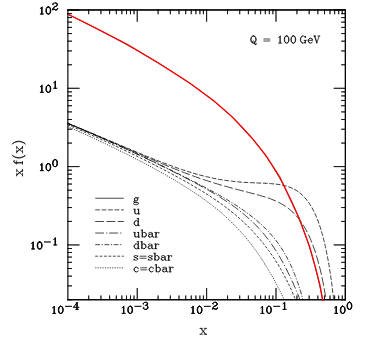
\includegraphics[width=0.55\linewidth]{Pics/cp1/PDF.png}
	\caption{ CTEQ6M PDFs  at an energy scale of $Q=100$~GeV. The different partons contributions are represented by the distributions $xf(x)$ and drawn vs the momentum fraction $x$ in a double logarithmic scale. The results are taken from~\cite{Pumplin:2002vw}.} 
	\label{fig:PDF}
\end{figure}


\section{Top-quark decay}\label{decay1}
Electroweak decay processes of the top-quark are predicted by the the Standard Model, where the top-quark produces new lighter quarks.  
The width of the top-quark decay is with $\Gamma_t$= 1.41~GeV~\cite{Olive:2016xmw} about one order of magnitude larger than the QCD energy breaking scale $\Lambda_{QCD}\approx$200~MeV. With its short lifetime, the top-quark decays even before  
hadronization can take place, thus no colour neutral top-hadrons can exist. Furthermore,  it is impossible to measure the top-quark properties directly. Only its decay products can be observed. Therefore, the top-quark decay plays an  important role for the investigation of the corresponding properties.


 In terms of the electroweak interaction, the explicit decay channels and the corresponding transition probabilities, are determined by the CKM-matrix elements (see~\cref{CKM}). The measured results, which have to be considered in terms of the top-quark are: $|V_{tb}| \approx$ 0.999,  $|V_{ts}|\approx$ 0.04 and  $|V_{td}|\approx$ 0.008~\cite{Olive:2016xmw}. 
As it can be seen by the coefficients, the decay into a bottom quark and a $W$-boson ($t \rightarrow b + W^+ $) is preferred, while the decays into a strange quark ($t \rightarrow s + W^+ $) or  a down quark ($t \rightarrow d + W^+ $) are strongly suppressed. The different decays can be further subdivided by the decay of the $W$-boson, which leads to important identification characteristics. The $W$-boson decays either into a charged lepton and the corresponding neutrino (e.g. $W^+\rightarrow l^+ + \nu_l$), or into a up-type quark and a down-type antiquark  (e.g. $W^+\rightarrow q + \bar{q'}$). 

\begin{figure}[h]
	\centering
	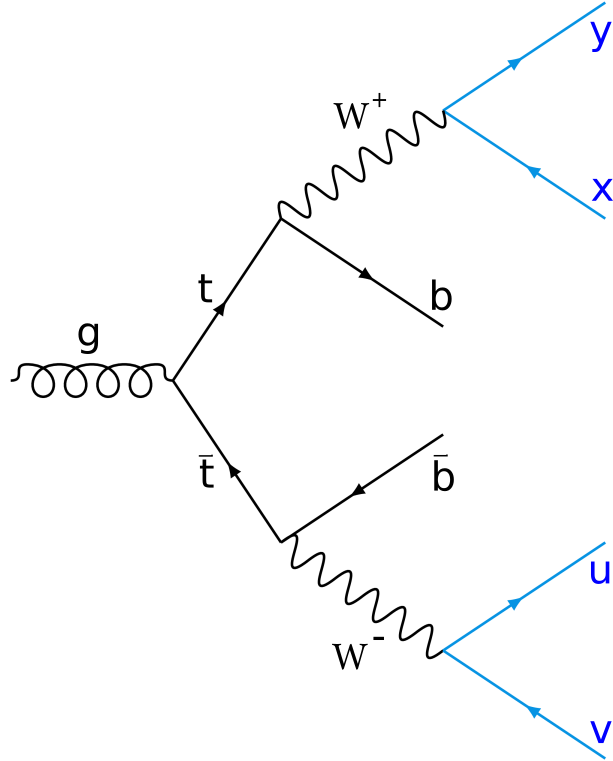
\includegraphics[width=0.3\linewidth]{Pics/cp1/Decay}
	\caption{Schematic decay of a $t\bar{t}$ pair. In the final decay state, the pairs xy and uv can be either quark or lepton pairs.  }
	\label{fig:Decay}
\end{figure}

 Based on the decays of the $W$-boson, the top-quark decay can be classified into three different decay channels, which are used for separate analyses, taking the specific signature inside the detector and the different background contaminations into account. The different decay channels are introduced below and  the corresponding branching ratios are given in~\cref{tab:T22}. The total decay chain is illustrated in~\cref{fig:Decay}, where the  $t\bar{t}$ pair is produced via  gluon-gluon fusion and  decays into the objects, which can finally be observed with the experimental equipment. The nature of these objects characterise the decay channel. They are denoted by the pairs x,y and u,v, which can either by a lepton or a quark pair.




\subsubsection{The all-hadronic decay channel}
In the fully hadronic decay channel (all-jets), both $W$-bosons from the $t\bar{t}$ final state decay hadronically into quarks. This is the dominant decay process for $t\bar{t}$ events. 

 Inside the detector, the signal of this decay is characterized by six jets. There are two jets  from the bottom quarks ($b$-jets), plus four lighter jets from the hadronic $W$-boson decays. The dominant background  for this decay channel stems from QCD-multijet events.

\subsubsection{The dileptonic decay channel}
With a branching ratio of just 10.5\% the dileptonic decay (dilepton) of both $W$-bosons is the smallest decay channel. 

 In the detector, this channel can be identified by a  signature with two $b$-jets from the top decays, two isolated charged leptons of opposite charge and a large amount of missing transverse energy, which is  a consequence of the two neutrinos.
The missing energy makes the reconstruction of this event topology particularly difficult. While QCD-multijet events do not play an important role, the dileptonic decay channel suffers from background from $Z$-boson events with extra jets in the final state.   

\subsubsection{The lepton + jets  decay channel}
The channel which is subject of the studies presented here, is  known as lepton + jets decay channel. One $W$-boson decays hadronically and  the other one leptonically, which offers significant advantages for the event selection and reconstruction. The leptonic  part of the decay helps to improve the identification of the interesting   events, while for the full kinematic reconstruction of the event the hadronic contributions are used in addition to the leptonic decay. 

 The detector signature consists of two $b$-jets and two lighter jets, one isolated charged lepton and a certain amount of missing transverse energy from the neutrino. Final states with a $W$-boson plus jets are the main background contribution for this decay channel.   
  

 \begin{center}
\captionof{table}{  Integrated branching ratios of the different top-quark pair decay channels~\cite{Olive:2016xmw}. }\label{tab:T22}

	
\vspace{0.3cm}	
	

\begin{tabular}{>{\centering}m{3.5cm}>{\centering}m{7.5cm} >{\centering}m{3.5cm} } \toprule

Decay channel& & Branching ratio&
\midrule
all-hadronic&$pp\rightarrow t\bar{t}\rightarrow W^+bW^-\bar{b}\rightarrow bq\bar{q'} \bar{b}q\bar{q'}$	&45.7\% &
dilepton	&$ pp\rightarrow t\bar{t}\rightarrow W^+bW^-\bar{b}\rightarrow bl\bar{\nu} \bar{b}\bar{l}\nu$&10.5\% &
lepton + jets		& $pp\rightarrow t\bar{t}\rightarrow W^+bW^-\bar{b}\rightarrow bl\bar{\nu} \bar{b}q\bar{q'}$&43.8\% &
\bottomrule
\end{tabular}

\end{center}
 \vspace{0.5cm} 
  
  
  
  
  
  
  
  
  

\chapter{The ATLAS experiment at the LHC}\label{ch3}

The production of massive particles, i.e. top quarks, requires a huge amount of energy. 
Therefore, powerful particle accelerators have been developed for the collision of high energetic initial particles. The kinetic energy of these particles has been used for the creation of new objects. Furthermore, complex experimental setups have been constructed to measure the results of those collisions and hence providing data, which is used for the reconstruction of the initial states of interesting events (e.g. $t\bar{t}$ production).

 The dataset used in terms of this analysis has been taken in the year 2016 with the ATLAS experiment, in proton-proton collisions, produced by the Large Hadron Collider (LHC), with a center-of-mass energy of 13~TeV. In this chapter the LHC, the ATLAS detector and its subdetector parts will be briefly introduced. Furthermore, a closer description of the trigger and data acquisition system is given as well. 




\section{The Large Hadron Collider}\label{LHC}
\vspace{0.5cm}
\begin{figure}[h]
\centering
\includegraphics[width=1.0\linewidth]{Pics/cp3/31}
\caption{Schematic view of the LHC and its location is given by (a) from reference~\cite{Bruning:2012zz}. The photograph (b) shows a section of the installed LHC in the  tunnel and was made by M. Brice~\cite{Brice:2221112}. }
\label{fig:31}
\end{figure}

 The Large Hadron Collider~\cite{Bruning:2012zz,Bruning:2004ej,Evans:2008zzb} is todays largest and most powerful particle accelerator. It is installed in the underground facilities of the previous Large Electron-Positron Collider (LEP)~\cite{LEP}, which retired after eleven years of operation in the year 2000. The circular tunnel system has a circumference of approximately 27~km and lies between 45 and 170~m below the franco-swiss border, close to Geneva (see~\cref{fig:31} (a) and (b)). In order to accelerate and collide particles with the same charge, the LHC consists of two beam pipes, which are crossing at four interaction points. In this setup proton-proton ($p-p$), lead-lead ($Pb-Pb$) or proton-lead ($p-Pb$) collisions are performed at the four main LHC experiments: \textbf{ATLAS, CMS, ALICE} and \textbf{LHCb}.

 The two multipurpose detectors ATLAS\footnote{A Toroidal LHC ApparatuS}~\cite{Aad:2008zzm} and CMS\footnote{Compact-Muon-Solenoid}~\cite{Chatrchyan:2008aa} are used for high precision measurements of the Standard Model parameters and the search for new physics. ALICE\footnote{A Large Ion Collider Experiment}~\cite{Aamodt:2008zz} is operating to collect data from heavy ion collisions, for the investigation of the quark-gluon plasma and LHCb\footnote{Large Hadron Collider beauty}~\cite{Alves:2008zz} is built for the search of rare decays and the investigation of CP-violation in the boosted $b\bar{b}$-system. In addition to the four main experiments, placed at the collision points of the LHC, there are the two smaller ones LHCf\footnote{Large Hadron forward}~\cite{Adriani:2008zz} and TOTEM\footnote{Total Elastic and Diffractive Cross Section Measurement}~\cite{Anelli:2008zza}, working on diffractive physics. At last there is the MoEDAL\footnote{Monopole and Exotics Detector at the LHC} experiment~\cite{Pinfold:2009oia}, which focuses on  the search of magnetic monopoles. 
\begin{figure}[h]
	\centering
	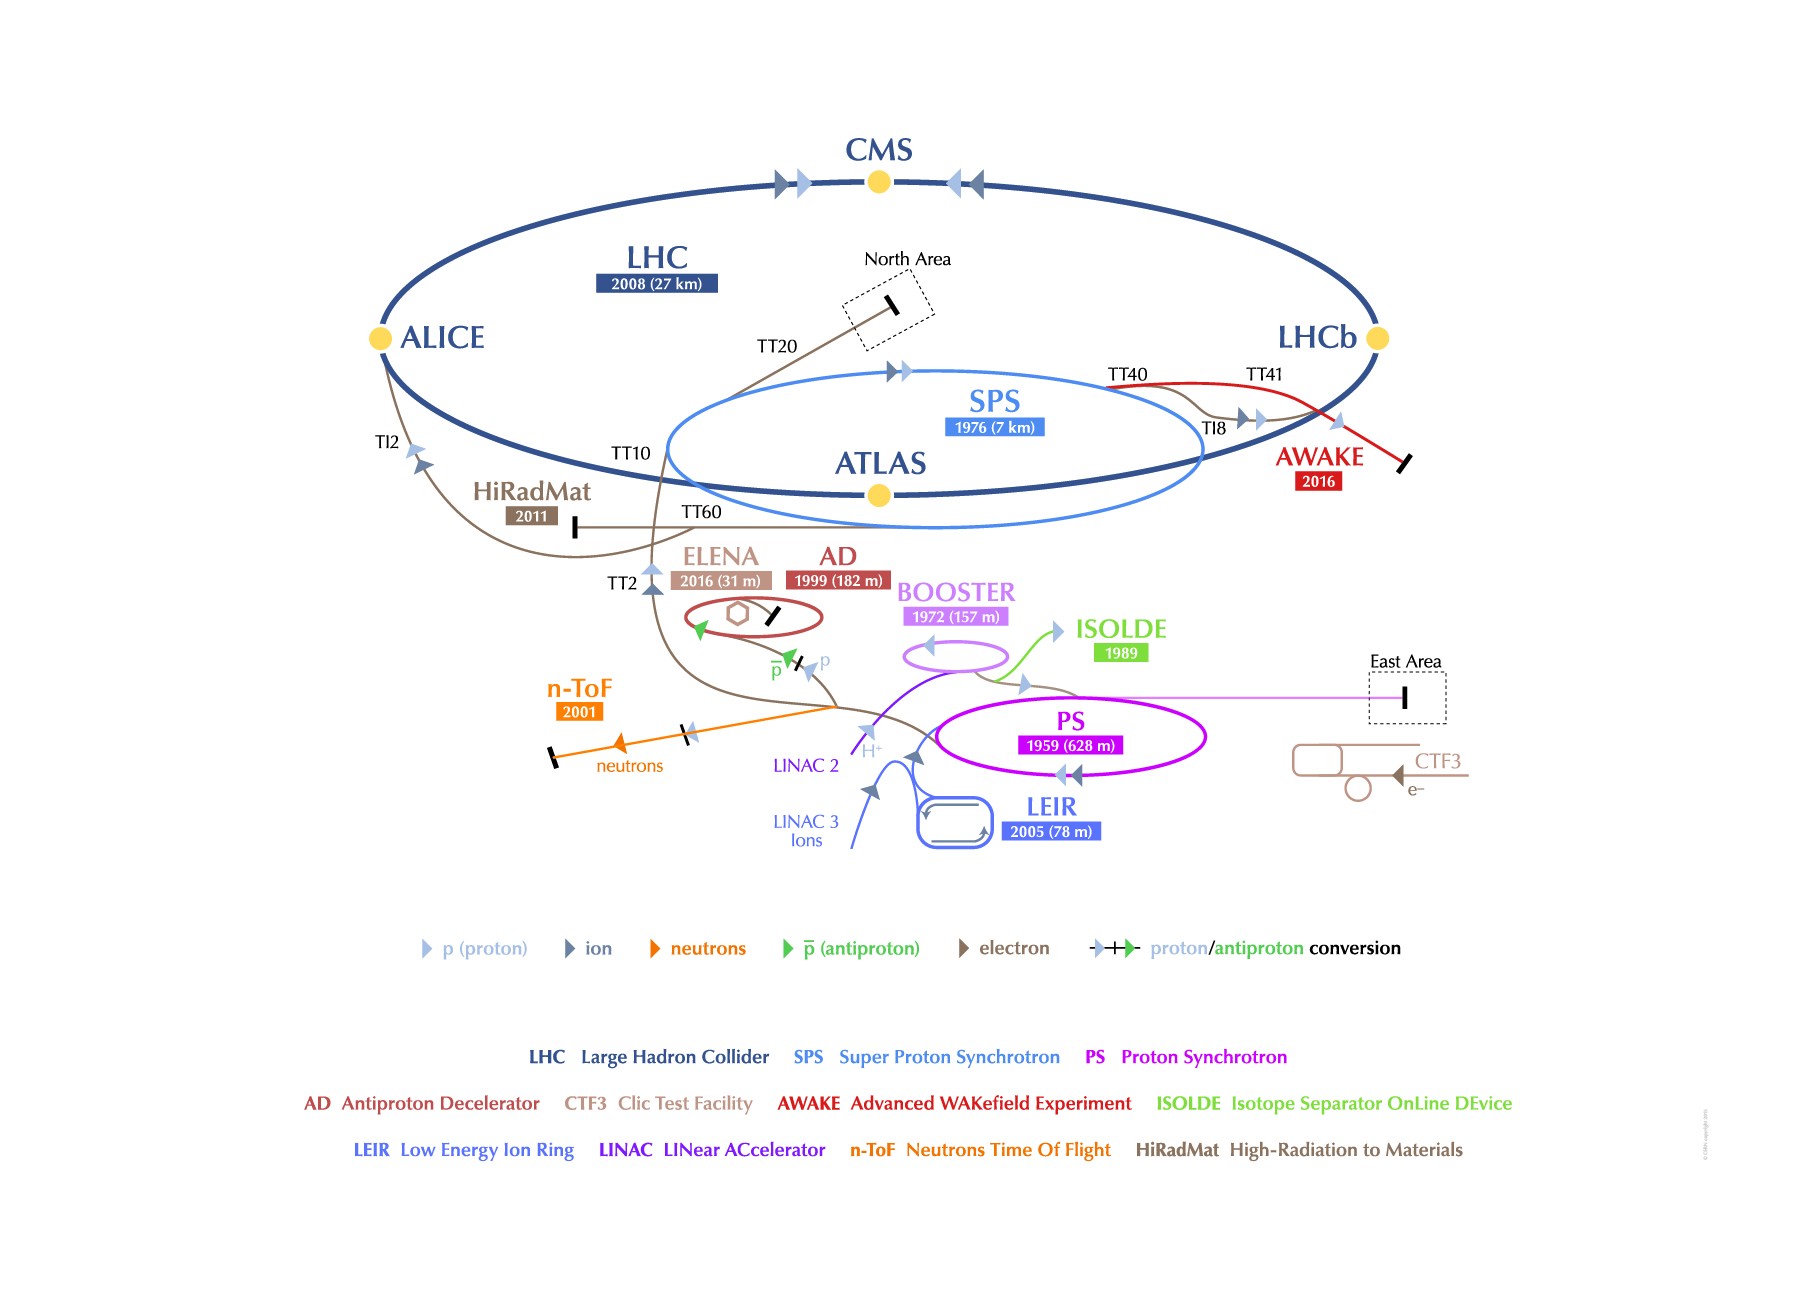
\includegraphics[width=1.0\linewidth]{Pics/cp3/32}
	\caption{Illustration of the whole CERN accelerator complex, with the complete pre-acceleration chain of the LHC~\cite{DeMelis:2119882}.} 
	\label{fig:32}
\end{figure}

 Before the initial particles are brought to collision in the LHC, they first have to pass a chain of pre-accelerators, which is illustrated by~\cref{fig:32}. Protons  are obtained from ionized hydrogen gas and injected in the first accelerator \textbf{LINAC2}, where they are accelerated to an energy of 50~MeV. The next acceleration step is done by the \textbf{Proton Synchrotron Booster (PBS)} that amplifies the proton energies towards 1.4~GeV, followed by the \textbf{Proton Synchrotron (PS)} and the {Super Proton Synchrotron (SPS)}, where the protons reach energies of 25~GeV in the first one and finally 450~GeV in the later one. After the SPS, the particles are injected into the {LHC}, where the acceleration continues up to the peak energy of currently 6.5~TeV.

 These accelerated protons, in each beam-pipe of the LHC, are grouped into bunches of 10$^{11}$ particles with a bunch spacing of 25~ns. These bunches are accelerated in the LHC by sixteen superconducting radio-frequency cavities. 1232 main superconducting dipole magnets and 392 main superconducting quadruple magnets are used for the guiding and the focusing of the particle beams along the beam-pipe. These magnets are cooled by superfluid helium below 2~K and a have a maximal field strength above 8~TeV~\cite{Evans:2008zzb}.   


 The LHC  exceeds all experiences of previous experiments,  in terms of luminosity. The peak luminosity is defined by:
\begin{equation}
\mathscr{L} = \frac{\gamma N_1N_2n_1n_2f}{4\pi \sigma_x \sigma_y }.
\end{equation}
 It depends on the number of particles $N_i$ in each bunch, as well as of the total number of bunches $n_i$ in the LHC, the revolution frequency $f$ and the cross-sections $\sigma_i$ of the incoming particle bunches. $\gamma$ denotes the relativistic coefficient. Design goal for the LHC has been to achieve a peak luminosity of $O$($10^{34}$~1/cm$^2$s$^{-1}$), at a center-of-mass energy of 14~TeV~\cite{Bruning:2004ej}. For 2015/2016 at 13~TeV the peak luminosity was 1.38$\cdot$10$^{34}$~1/cm$^2$s$^{-1}$.  
 
 
\section{The ATLAS experiment}\label{ATLAS}
 ATLAS  is one of the two multipurpose detectors at the LHC and has obtained the dataset used in this analysis. It measures 44~m in length and 25~m in diameter and weighs around 7000~t~\cite{Aad:2008zzm}. 
 As shown by~\cref{fig:33}, it covers almost a full 4$\pi$ solid angle and has a forward-backward symmetry, which is realized by the so-called barrel around the collision center and the two end-caps. The detector is built up with an onion-shell structure, consisting of various sub-detector layers. The three main subcomponents of the ATLAS detector are:
 \begin{itemize}
 	\item the \textbf{Inner Detector system (ID)}, for the reconstruction of particle trajectories, 
 	\item  the \textbf{Calorimeter System (CS)}, which is measuring particle energies
 	\item  and the \textbf{Muon Spectrometer (MS)}, for the determination of the muon momentum.
 \end{itemize} 
Characteristic for the ATLAS experiment is the huge superconducting air-core toroid system, which is used for the deflection of muons in the MS. 

 The different detector components are optimized in order to identify and distinguish between the different constituents of a collision, facing difficulties like high particle multiplicities and high event rates. Therefore,  additionally  efficient triggering and fast read-out electronics is required, to distinguish between background and signal.

The different layers of the ATLAS experiment will be briefly discussed after a short introduction of the detector coordinate system. For a more detailed information, the reader should read~\cite{Aad:2008zzm,ATLAS:1999uwa}.   


\begin{figure}[t]
	\centering
	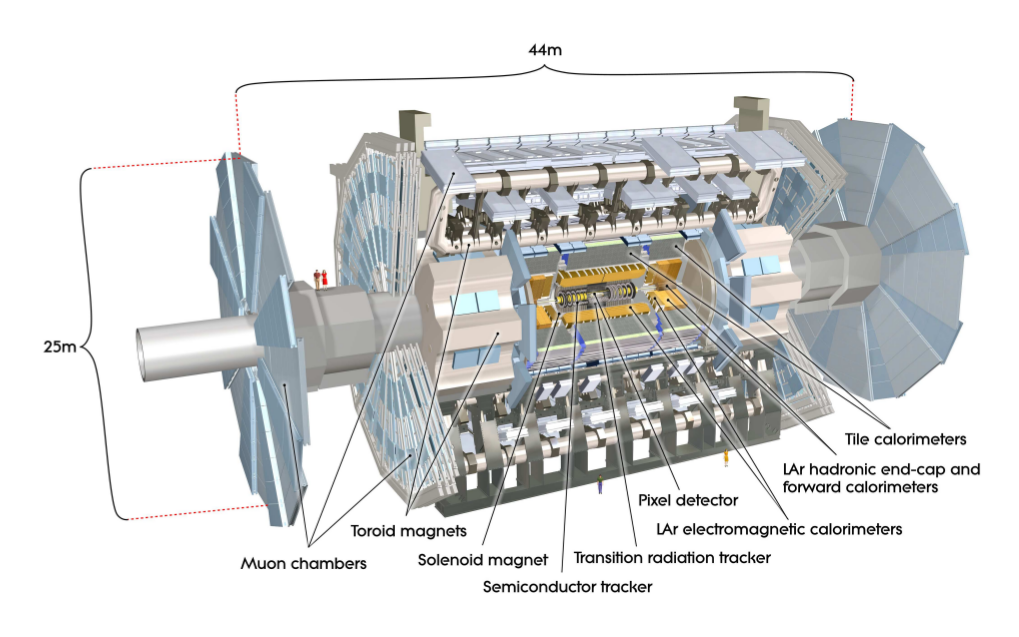
\includegraphics[width=1.0\linewidth]{Pics/cp3/33}
	\caption{The ATLAS experiment and its sub-structure~\cite{Aad:2008zzm}.} 
	\label{fig:33}
\end{figure}



\subsubsection{The coordinate system }\label{Coordinate}
The cylindrical shape of the ATLAS experiment implies the use of a common coordinate system, which has its origin at the interaction point of the initial particles. 
The z-axis lies parallel to the LHC beam-pipe, while the  x-y plane (the so-called transverse plane)  is perpendicular to it, with the x-axis pointing inwards to the LHC center and the y-axis pointing to the surface of the earth.  Often the r-$\phi$ coordinates are used in the transverse plane.
 $\phi$ denotes the azimuthal angle, which is defined  around the beam-pipe with respect to the x-axis.
 The distance of a coordinate in the transverse plane to the beam-pipe, is given by r.  
 In addition, the polar angle ($\theta$), which is measured  with respect to the positive z-axis, is used to define the so-called pseudorapidity:
\begin{equation}\label{pseudorapidity}\eta = -\text{ln}\left(\text{tan}\left(\frac{\Theta}{2}\right)\right).
\end{equation}  
 For the interesting central detector region, close to the y-axis, $\mid\eta\mid$ takes low values and offers a high resolution, while in the background dominated section $\mid\eta\mid$ increases rapidly with declining distance to the beam pipe. Thus, this high $\mid\eta\mid$  region is often excluded in the measurements. In addition, the introduction of the pseudorapidity provides with $\Delta \eta$ -the distance between to distinguishable values- a quantity which is invariant under Lorentz transformations along the z-axis. Furthermore, for massless objects, the pseudorapidity is equal to the so-called rapidity, which is defined as:
\begin{equation}\label{rapidity}
y = \frac{1}{2}\text{ln}\left(\frac{E + p_z}{E - p_z}\right).
\end{equation}
$E$ denotes the energy and $p_z$ the third component of the particle momentum. The rapidity is invariant under Lorentz transformations. 


The distance of two different particles $i$ and $j$ can be described by:
\begin{equation}\label{dinstance}
\Delta R_{i,j} = \sqrt{(\eta_i-\eta_j)^2+(\Theta_i-\Theta_j)^2}.
\end{equation}
   

The hadron sub-structure gives rise to further issues. The momentum fraction $x$ carried by the different partons can not be determined exactly, because the parton density functions allow only to determine the probability that a parton has a certain momentum fraction. Therefore, the absolute values of the parton momentum and the corresponding energy are unknown. 
However, the initial particles are accelerated along the z-axis and the transverse energy ($E_T$), as well as the corresponding transverse momenta ( $p_T$) are zero.
Therefore, it can be  assumed that the transfers components for the final state particles also sum up to zero.  The transverse momentum can be calculated with: 
 \begin{equation}
 p_T = \sqrt{p_x^2+p_y^2}.
 \end{equation}  
 More information about the transverse energy can be found in~\cref{ET}.        





\subsection{The Inner Detector System}\label{ID}
The Inner Detector System (ID) of the ATLAS experiment, is designed to reconstruct the tracks, as well as the primary and secondary vertices, by the interaction of the charged particles with the detector material. Therefore, the ID consists out of three sub-components, which are designed to provide a high vertex and momentum resolution, due to  very fine granular structures.

The whole ID system is composed out of a cylindrical part, located in the barrel around the collision point, and the corresponding detector end-caps. It measures around 7~m in length and has a diameter of 2.3~m. The complete ID is contained in a solenoidal magnetic field of 2~T, which is used for the bending of charged objects and resolving the sign of the charge. The required precise resolution is realized by the use of discrete space-points from several silicon pixel layers at the most inner region of the ID (see~\cref{fig:34}).

 The \textbf{Silicon Pixel Detector}, closest to the collision center, is built out of three layers parallel and three disks perpendicular to the beam pipe, with 1744 sensor modules in total. It is mainly used together with the \textbf{Semiconductor Tracker (SCT)}, which is installed in the layers above for the momentum measurement and the vertex reconstruction. The SCT consists of four silicon strip layers in the barrel and  eighteen disks in both end-caps. This results in a total number of 3100 modules. The 12~cm silicon strips are composed of two connected sensors, often refereed as dual layer design. The sensors are connected with readout electronics.

 At the outer radii of the ID, the \textbf{Transition Radiation Tracker (TRT)} is placed.
It uses the information arising from the transition radiation of passing particles, to distinguish e.g. between electrons and pions. The TRT is built out of several layers of straw tubes filled with a gas mixture of XeCO$_2$ and O$_2$. While the TRT is constructed to operate at room temperature, the silicon sensors of the detector have to be cooled down between -5 and -10~\textdegree C, to get a satisfactory noise performance and long term reliability, while suffering under the high radiation close to the beam-pipe~\cite{Aad:2008zzm}.     
\begin{figure}[t]
	\centering
	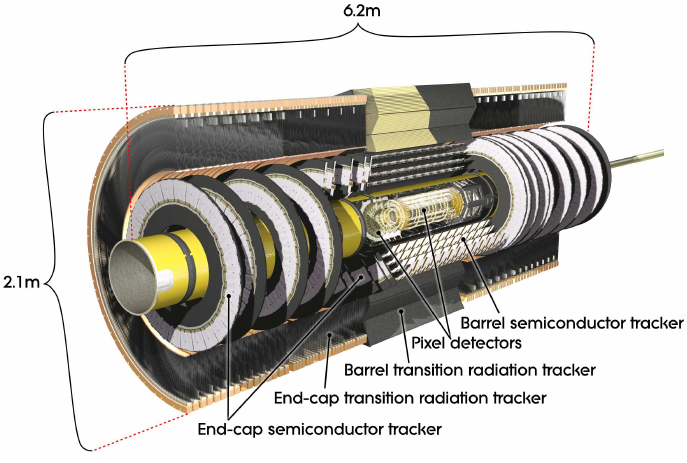
\includegraphics[width=0.7\linewidth]{Pics/cp3/34}
	\caption{Cut through the Inner Detector System~\cite{Aad:2008zzm}.} 
	\label{fig:34}
\end{figure}

\subsection{The Calorimeter System}\label{CD}




The second detector shell is specifically developed for the measurement of energies induced by particle showers, also known as clusters. 
Electrons, positrons and photons deposit most of their energy in the inner layer, which is called the \textbf{Electromagnetic Calorimeter (EC)}.  The particles interact with the  detector material, e.g. via electron-positron pair production and annihilation or the radiation of bremsstrahlung. Thus, secondary particles are triggered by the passing ones, resulting in electromagnetic showers. If the incident particles are hadrons, the same phenomenon occurs, due to inelastic scattering  of the hadrons with the nuclei of the detector material. The scattering processes lead to the production of new hadrons, which participate in further interactions and therefore creating a hadronic particle shower, which is also detected by the EC and in addition by the outer \textbf{Hadronic Calorimeter (HC)}. Despite the energy measurement, the Calorimeter System also allows to determine the particle momentum and identity by the analysis of the direction and the spatial characteristics of the induced clusters.

The Calorimeter System has a  cylindrical shape, which measures 12.20~m in length with radius of 4.25~m (see~\cref{fig:35}). It is built out of so-called sampling detectors, which are alternating structures of layers with a passive and an active component.

 The passive material interacts with the incident particles and triggers the particle shower, while the active material gets ionized by the passing particles from the shower and provides information for the electronic read out. In case of the ATLAS Calorimeter System, liquid argon (LAr) is the preferred choice for the active part, because of the intrinsic linear response and the excellent radiation hardness~\cite{Aad:2008zzm}. A cryogenic system is used for a constant operational temperature of 87~K.


\begin{figure}[h]
	\centering
	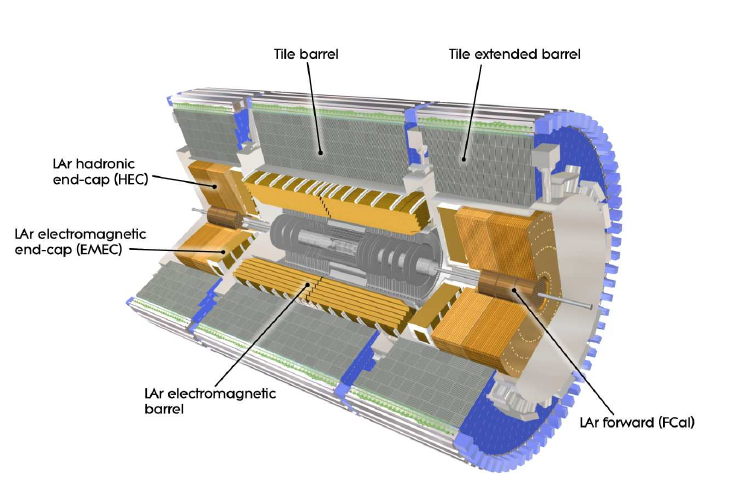
\includegraphics[width=0.65\linewidth]{Pics/cp3/35}
	\caption{Cut through the Calorimeter  System~\cite{Aad:2008zzm}.} 
	\label{fig:35}
	\end{figure}



 The \textbf{Electromagnetic Calorimeter} is built out of two units with a length of 3.2~m in the barrel region, plus two end-cap wheels. Lead is used for the passive and liquid argon for the active media. The kapton electrode layers have a characteristic accordion shape, which allows to cover a decent $\Phi$  and $\mid\eta\mid$ range, e.g. the area for high precision measurements  ($0 \leq~  \mid\eta\mid ~\leq 2.5$) is covered, as well as the high-$\eta$ area  ($2.5 \leq~ \mid\eta\mid~ \leq3.2$). In front of the EC, a presampling layer is installed to measure energy losses  from particle interactions with the ID and the beam pipe.




For the detection of particle showers from quarks and gluons the \textbf{Hadronic Calorimater}. While both calorimeters are used for the observation of hadron jets, the most amount of energy is deposited in the latter one, which uses scintillator tiles and steel absorbers in the inner region. In this so called \textbf{Tile Calorimeter (TC)}, the scintillators act as active media, which creates photons by the interaction with the incident particles. Wavelength shifters and photomultipliers are  used for the generation and amplification of the electrical signal. The TC has a inner radius of 2.28~m and a outer one of 4.25~m. It is built out of a central barrel with a length of 5.8~m, plus two extended barrels, measuring 2.6~m in length. This construction  allows to cover a pseudorapidity range of $0 \leq \mid\eta\mid \leq1.7$.

 Larger $\eta$ regions are taken into account by the \textbf{Hadronic End-Cap Calorimeter (HEC)} and the \textbf{Forward Calorimeter (FCal)}, which enable to observe a pseudrapidity range up to 4.9.  In the HEC, copper and liquid argon are used as sampling media. In each of the end-caps, two cylindrical HEC wheels with a radius of 2.03~m are embedded, resulting in the coverage of the section: $1.5 \leq \mid\eta\mid \leq3.2$.

 The FCal is placed in the same segment as the HEC, covering the $3.1 \leq \mid\eta\mid \leq 4.9$. It uses copper and tungsten for the passive sampler, combined with liquid argon for the active one. The mixture of the two passive media is chosen due to the high particle flux, which stresses the detector material extensively.




\subsection{The Muon Spectrometer}\label{MD}

\begin{figure}[h]
	\centering
	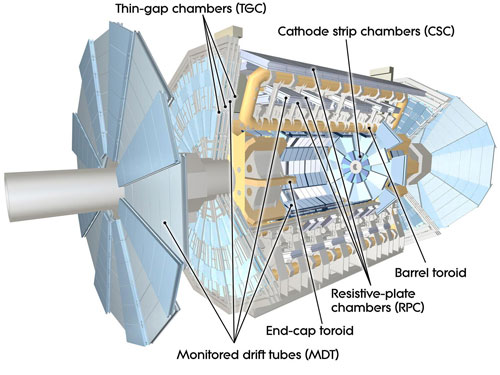
\includegraphics[width=0.65\linewidth]{Pics/cp3/36}
	\caption{The Muon Spectrometer with all its sub-components~\cite{Aad:2008zzm}.} 
	\label{fig:36}
\end{figure}

 The momenta of muons leaving the calorimeter are measured in the outer layer of the ATLAS experiment, the \textbf{Muon Spectrometer (MS)}. Together with the information provided from the Inner Detector System, the measurements of the MS can be used for the reconstruction of the muon trajectories. Furthermore, the MS works also as a trigger for events with muons.

The track reconstruction in the MS is based on the magnetic deflection of the muons by a large superconducting air-core toroid magnet system in combination with  trigger and tracking chambers. The design goal of the whole Muon Spectrometer is to achieve a momentum resolution of 10~\% for 1~TeV and up to 3~\% for 10-200~GeV muons~\cite{ATLAS:1999uwa}. The instrumentation design was mainly dictated by the high particle flux, which has huge impacts on the operational performance, considering e.g. aging and agglomeration of polymers, high rate capability and radiation hardness.

 The complete system (see~\cref{fig:36}) consists of three barrel layers with radii of  5~m, 7.5~m and 10~m, as well as of four end-cap wheels, located at $\mid z \mid$ = 7.4~m, 10.8~m, 14~m and 21.5~m. 
With increasing radii also the dimensions of the different layers and their components gain in size. In the barrel, as well as in the end-cap region, \textbf{Monitoral Drift Tubes (MDTs)} and \textbf{Cathode Strip Chambers (CSCs)} provide high spatial resolution, due to the fact, that the systems are monitored with an optical alignment system, which provides excellent spatial information. Moreover, \textbf{Resistive Plate Chambers (RPCs)} in the barrel and \textbf{Thin Gap Chambers (TGCs)} in the forward section are  installed for additional trigger information.



 For the magnetic bending of the muons, a unique superconducting \textbf{Magnetic System} is installed in the MS. Together with the solenoid of the ID, it allows the determination of the electromagnetic charge signs of the particles, as well as a high-precision measurement of the momenta. The MS system is composed of one large barrel toroid and two smaller toroids in the end-caps (see~\cref{fig:37}). It measures  26~m in length, with a diameter of 22~m and provides a specific magnetic field configuration, resulting in orthogonal alignment of the field towards the muon trajectory~\cite{ATLAS:1999uwa}. In the transition region, between barrel and end-caps, the magnetic field is reduced, while in general it is  non-uniform distributed  with a field strength of 4.7~T.  A cryogenic system with liquid helium is used to cool down the system to 1.8~K. Furthermore,  each coil has an air core, for the noise reduction due to  multiple scattering processes of the muons. 

\begin{figure}[h]
	\centering
	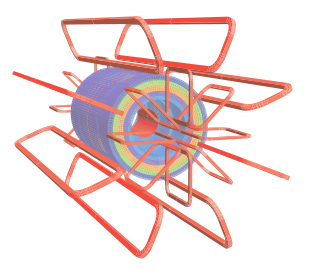
\includegraphics[width=0.4\linewidth]{Pics/cp3/37}
	\caption{Illustration of the ATLAS Magnet System, with the inner solenoid of ID and the large superconducting coils of the MS ~\cite{Aad:2008zzm}.} 
	\label{fig:37}
\end{figure}



 The \textbf{Monitorial Drift Tube} System consists of rectangular  chambers, which measure between 1~m and 6~m in length and 1~m up to 2~m in width. The chambers contain several layers of cylindrical drift tubes, filled with a gas mixture of Ar (30~\%) and CO$_2$ (70~\%) at a nominal  pressure of 3~bar. Incident muons, ionize the the argon gas and create free electrons, which drift towards the central tungsten-rhenium anode wire of the tube, producing an electron avalanche.  The anode has a diameter of 50~$\mu$m and a potential of 3080~V. The end-plugs are designed to hold the wire in position with an accuracy smaller than 10~$\mu$m and are connected to the read out electronics. The CO$_2$ is used as quench gas, to eliminate additional interaction processes, which could for example arise from electrons ripped out of the cathode. 

 The use of MDTs is limited by the counting rates (150~Hz/cm$^2$), which are exceeded in the forward region. Therefore, MDTs are replaced by \textbf{Cathode Strip Chambers}, which are able to handle the high particle flux in the end-cap region by providing counting rates up to 1000~Hz/cm$^2$~\cite{ATLAS:1999uwa}. There are two disks in the detector wheels, each containing 8 CDCs. The CDCs are multi-wire proportional chambers, with cathode strips  and anode wires orientated in radial direction. The chambers are filled with a gas mixture of  80~\% Ar and 20~\% CO$_2$, acting as quench gas. The track reconstruction is based on the information of induced charge in the anode wires, created by the ionized argon.

 For the particle triggering, three trigger layers of \textbf{Resistive Plate Chambers (RPC)}, are embedded  in between the MDTs. Each of these so-called trigger stations consist of two separate sub-layers. Thus a particle passing trough provides multiple informations, which help to reduce noise.  The RPCs are parallel-plate detectors, where electron avalanches are formed by an electrical field (49~kV/m) between two electrodes, which are  2~mm separated to the insulating material. The RPCs are filled with a gas mixture of 94.7~\%   C$_2$H$_2$F$_4$, 5~\% Iso-C$_4$H$_{10}$ and 0.3~\% SF$_6$, which allows for example to work with  low voltages~\cite{ATLAS:1999uwa}. 

Additional trigger information in the end-cap regions is obtained by \textbf{Thin Gap Chambers (TGCs)}. These are multi-wire proportional counters, where the anode wires 
measure the radial coordinate of the particle track and outer strip electrodes provide the azimuthal information. The ATLAS TGCs are operating a gas combination of CO$_2$ and n-C$_5$H$_{12}$, which offer high quench capabilities.


\section{Trigger system and data acquisition}


 The amount of information produced due to the  high luminosity and large bunch-crossing rate of 40~Mhz at the LHC, makes it impossible to store all the data. Furthermore, only a fraction of all interactions result in interesting events, e.g. $t\bar{t}$ production. Therefore, the ATLAS collaboration works with a \textbf{three level trigger system}. The so-called trigger stations consist of a hardware-based Level 1 trigger (L1), the software based Level 2 trigger (L2) and the Event Filter (EF). For the second run period of the LHC (Run 2), the L2 trigger and the Event Filter are merged in  the~\text{High Level Trigger} (HLT). In order to reduce the complexity of the system the following explanation will stick to the three levels of the trigger system. The complete trigger system is illustrated in~\cref{fig:38}. For the data storage, as well as for the further analysis, the \textbf{Worldwide LHC Computing Grid} is used.

\begin{figure}[t]
	\centering
	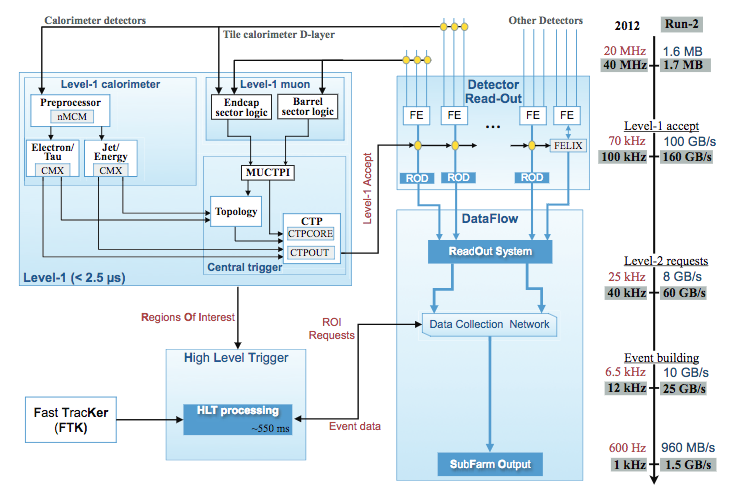
\includegraphics[width=0.80\linewidth]{trigger}
	\caption{Sketch of the three level trigger system~\cite{Nakahama:2015211}.} 
	\label{fig:38}
\end{figure}


 The entirely hardware based \textbf{L1} trigger station uses for its selection, information from the Calorimeter System and from the Muon Spectrometer. L1 searches for high $p_T$ muons, electrons, jets and missing transverse energy. This data is used for the definition of Regions of Interests (RoIs), which will be used for the further refinement and selection by the next trigger stations. Therefore, the events are stored in so-called Read-Out-Drivers (RODs). It takes 2.5~$\mu$s, for the complete selection of the RoIs, which leads to a reduction of the event rate towards 100~kHz. The second trigger station \textbf{L2} is software-based and takes the complete detector information of the RoIs into account. For the selection of this trigger station large computational facilities are used. The event rate after L2 is reduced to 12~kHz. 
Events that survive this selection step, are passed to the Event Filter.

 The final step of the trigger process is the \textbf{EF}, where a full reconstruction of the different constituents of the event, with all available information, is performed. The physical objects and their properties, e.g.  tracks and vertices are rebuilt. At last the selected events are saved permanently. The final event rate after the EF is 1~kHz and the data rate is 1.5~GB/s~\cite{Nakahama:2015211}.






\subsection{Data handling}

 In order to handle the storage of the huge amount of data, as well as providing the necessary computational infrastructure, e.g. for Monte Carlo simulations, the\textbf{ Worldwide LHC Computing Grid (WLCG)} has been developed. It is based on large computational facilities around the globe, which are sharing their storage capabilities and processing power. This computer network is structured into different hierarchies, where the CERN computing center has the highest, so-called  Tier-0,  rank. There are stored copies of all raw data sets. Furthermore, there are backups at eleven computer centres around the globe, which are the so-called Tier-1 centers. Moreover,  the smaller Tier-2 centers are used to store copies of selected data and to provide the necessary resources for the data analysis and the simulation of events via Monte Carlo generators. The datasets are stored in streams and reconstructed within 24h.


\subsection{Detector simulation}
This analysis uses the template method, which is based on simulated Monte Carlo distributions. In order to compare the simulated events to measured data, a detailed simulation of the ATLAS detector has been developed by the ATLAS collaboration (see~\cite{Aad:2010ah}). 
The detector simulation is based on the \text{Geant4}~\cite{Agostinelli:2002hh} program  and starts from the event generation. The provided output of the simulation has a format, which can be compared to the data measured with the real detector.  

 
 The first step is the event generation, where a set of particles is produced and passed through the detector simulation. 
For the event generation, several standard physic generators can be used. 
 The generated events consist of particles  related to a single interaction, where the corresponding vertex is located at the geometric origin. 
 Particles which have a decent lifetime (about 30~ps) are treated as stable particles. These particles are considered to be able to interact with the detector material and their decay is taken into account by the simulation. For short living particles, the decays are handled by the event generator itself. The corresponding interactions with the detector material are ignored.  
The core simulation within  \text{Geant4} models the particle transportation through the detector geometry and takes additional information provided by the user into account. The hits,  produced by the simulation, are converted into detector responses. These so called digits are produced  if the corresponding electrical signal in the readout-channels exceeds a defined threshold in a certain time range. ~\cite{Aad:2010ah} 

After the detector simulation, the simulated data is passed through the same event reconstruction software as the data.
A correct simulation of the detector is generally  important for the physic analysis. Deviations in the simulation can  for example be observed by comparing the data to the simulation.

\chapter{Object definition and preselection}\label{ch4}


The $t\bar{t}$ pairs, produced in proton-proton collisions at the LHC, decay immediately after their creation and leave a unique signature in the detector, which allows to distinguish the interesting events from the physical background. However, the observed signature in the detector gives only hints about the decay products of the top-quark pair.
In the case of the lepton + jets channel, these decay products are electrons, muons, jets and a certain amount of missing transverse energy, corresponding to the neutrino. In order to identify these objects, one has to introduce a definition of the different physical objects which are required for measurements. Hence, the decay products of the $t\bar{t}$ final states are connected with the quantities measured by the experiment.

All definitions which are used in terms of this analysis are introduced in the following, after a short consideration of the general event topology. In addition, the used data and simulation samples are described, as well as the different background processes. Finally, the chosen event selection cuts are shown.
\section{Physics objects}
\subsection{Total event topology}

For the general reconstruction of events arising from particle collisions at the LHC, the very complex nature of the event topology and the underlying processes have to be considered.
Additional activities in the detector make it difficult to identify specific physical objects. Furthermore, a lot of processes have a similar event structure to the one of the $t\bar{t} \rightarrow$ lepton + jets channel.  


 For example, there is the so called  \textbf{beam remnant}, that names background processes arising from partons which do not take part in hard interactions. These partons are colour connected with the hard scattered partons. The colour connection results from the QCD confinement, which requires colour neutral  $SU(3)_C$ singlets (hadrons). Secondly, further background contamination arises from \textbf{multi parton interactions} between partons of the same proton. At last, noticeable contributions can be observed due to
further interactions of different proton-proton interactions as a consequence of the high luminosity of the LHC.
If these interactions appear in the same bunch-crossing  as the hard interaction which contains the event of interest, it is called \textbf{in-time pile-up}, while processes  which originate from consecutive bunch-crossings are known as \textbf{out-of-time pile-up}. 
      
These additional processes are overlaying with the interactions of interest. The reduction of pile-up contamination is a challenging task and is important not only for  a good event reconstruction, but also for the correct identification of the physical objects. 

\subsection{Electron candidates}   
Electron candidates are reconstructed with the information provided by the Electromagnetic Calorimeter (EC) and the Inner Detector (ID). The sliding-window algorithm is used to seed and reconstruct electromagnetic clusters with a deposited energy of at least 2.5~GeV~\cite{Aad:2014fxa}. The measured transverse energy in the EC, along the trajectory of the possible electron is defined as
\begin{equation}
	E_T= \frac{E_{\rm cluster}}{\rm cos(\eta)},
\end{equation} 
where $E_{\rm cluster}$ denotes the total observed energy of the cluster. The reconstructed calorimeter clusters can be characterized by the $E/p$ ratio, the shower shape and the leakage into the Hadronic Calorimeter.
  
For so called \textbf{loose} electrons, only the shower shape inside the EC and the leakage of the electromagnetic jet into the Hadronic Calorimeter are taken into account. \textbf{Medium} electrons require the same conditions as loose ones. In addition particle tracks measured by the ID are matched to corresponding signatures of electromagnetic shower in the EC. Furthermore, specific quality criteria, which are analysis dependent, are applied. The last category are  \textbf{tight} electrons, which are satisfying the medium electron conditions with tighter restrictions on the   matching between the  trajectory of the ID and the EC cluster. Furthermore, additional information from further detector components, like the  transition radiation trackers, is used.~\cite{Aad:2011mk} 

 For this analysis, electron candidates have to fall into the tight category with  a transverse energy of at least 27~GeV. Furthermore, only clusters within a pseudorapidity range of $0 < \mid\eta_{cluster}\mid < 2.47$ are accepted. Objects in the transition region between the electromagnetic calorimeter barrel and the end-caps $1.37 < \mid\eta_{cluster}\mid < 1.52$, the so-called crack region, are excluded. Nevertheless, there are leptons which can be mis-identified with the so-called prompt leptons of the hard scattering process of interest, while they actually arise from different processes. These  non-prompt leptons  (NP) result e.g. from heavy-flavour decays inside of jets or from photon conversions. Furthermore, also hadronic particle showers can lead to an electromagnetic  detector signature. This is known as fake-leptons and will be discussed in~\cref{selection}. In order to minimize the influence of this so called NP/fake-lepton background contamination, electron candidates have to fulfil certain isolation criteria.


 Therefore, specific isolation variables quantify the energy of the particles produced around the electron candidate and allow the separation of prompt electrons from non-isolated electron candidates.  The first variable is  the calorimetric isolation energy $E_T$.  This energy corresponds to a cone of  $\Delta R$ = 0.2, of the  topological calorimeter clusters, around the electron candidate. The sum over the energy of the chosen clusters has to be positive. There are corrections, which take care of the energy leakage outside of the cluster, as well as for the pile-up and the underlying events. The second variable is the track isolation $p_T$. It is defined by the total transverse momentum of all tracks which fulfil  certain quality requirements within a cone of $\Delta R =$ min(0.2~GeV/$E_T$) around the the track of the electron candidate. The source of the track has to be identified with the primary vertex of the hard interaction\footnote{The primary vertex is the one  with the highest   $\sum p_T^2$, where  $p_T$ denotes the transverse momentum and the sum runs over all associated  tracks.}. In addition, within the different cones, the $E_T$/$p_T$ has to be smaller than a certain threshold.~\cite{ATLAS:2016iqc}

 In addition to the isolation criteria, the impact parameter $d_0$, which is the closest measured distance of the track to the beam-line has to full fill: $d_0/\sigma_{d_0} <5$, where  $\sigma_{d_0}$ represents the estimated uncertainty of $d_0$. Furthermore, the distance $z_0$ along the beam-line, between the beam-spot position and the measured position of $d_0$,  is constrained together with the polar angle of the track to be: $\mid \Delta z_0 \text{sin}(\phi) \mid$ < 0.5~mm. ~\cite{ATLAS:2016iqc}







\subsection{Muon candidates}

At the LHC, muons are minimum ionizing particles. The corresponding mean energy deposition in the calorimeter system is small, e.g. compared to electrons or photons. Therefore, the Muon Spectrometer (MS) at the outer regions of the ATLAS experiment was installed, for a better reconstruction of muon candidates.  In principle muons can be reconstructed at the ATLAS experiment using just the information from the MS. In this case, the particle track is obtained by the MS and further deduced towards the collision point of the protons. For this purpose, the toroidal magnetic field, which encloses the MS, bends the particle tracks.  One refers to muons that are constructed in that way as \textbf{stand alone} muons. 
The success rate to identify muon candidates can be increased by the use of \textbf{combined} muons. For combined muons, the particles obtained with the MS are matched with tracks of the Inner Detector (ID) system, using the MuID reconstruction algorithm~\cite{Aad:2014rra}. Alternatively, one can require so-called \textbf{tagged} muons, where  promising ID tracks of possible muon candidates are searched for. These tracks are then approximated towards the outer MS layers, where events  close to the extrapolated tracks  are searched. For the studies presented in this thesis, combined muons are used.


 
 
For this analysis, \textbf{medium} muons are used to minimize the systematic uncertainties, which arise from the muon reconstruction and calibration~\cite{Aad:2016jkr}. The tracks of medium muons are identified using the information of the calorimeter system, where the  deposited energy has to match the energy deposition from  minimum ionizing particles. Additional information of the particle trajectory is obtained by the MS. A detailed definition, also for the alternative setups \textbf{loose}  and \textbf{tight}, can be found in~\cite{Aad:2016jkr}.
 

  
 The reconstruction of the combined muons with the MuID algorithm starts with the outermost layers of the Muon Spectrometer. The tracks are extrapolated towards the layers further inside, in several iteration steps. Potential sources of disturbances, e.g. interactions with the detector components, are also considered for the reconstruction. The information obtained from the MS is thus matched with the reconstructed tracks from the ID. Moreover, only central muons  within the interval of 0 < $\mid\eta\mid < $ 2.5 and with a $p_T>27$~GeV  are used for this analysis. In order to reject muons originating from heavy flavour decays, the muon candidates have to fulfil the isolation criteria, with two isolation variables.

 First of all, there is the track-based isolation variable, which is evaluated from the scalar sum of the transverse momentum, for tracks with $p_T$ > 1~GeV. Therefore, tracks with in a cone of $\Delta R =$ min(10~GeV/$p_T^{\rm muon}$, 0.3), around the muon with the transverse momentum $p_T^{\rm muon}$ are considered. Furthermore, the transverse energy of the calorimeter cluster, in a cone of $\Delta R$ = 0.2 around the muon candidate is taken into account. Therefore, corrections are applied by the subtraction of the energy deposition of the muon candidate itself, as well as for the impact of pile-up. 
For the detailed isolation selection, relative quantities are  used,  defined via the ratio of  the track/calorimeter isolation variables and the transverse momentum of the muon.~\cite{Aad:2016jkr}

 In addition, there are cuts on the significance of the transverse impact parameter  $d_0/\sigma_{d_0}$ < 3.0, as well as on the the longitudinal impact parameter $z_0$ < 10 mm and $\mid \Delta z_0 \text{sin}(\phi) \mid$ < 0.5~mm~\cite{Aad:2016jkr}.



\subsection{Jets}\label{JES}
Compared to electrons and muons, which can be treated as quasi-free particles, the reconstruction of objects, which interact via the strong interaction, is much more difficult. Due to the colour confinement, these particles trigger showers of colour-neutral hadrons. These hadron showers deposit their energy in the cells of the calorimeter system (see ~\cref{fig:41}), thus providing the information for the reconstruction of the quarks and gluons.

\begin{figure}[h]
  	\centering
  	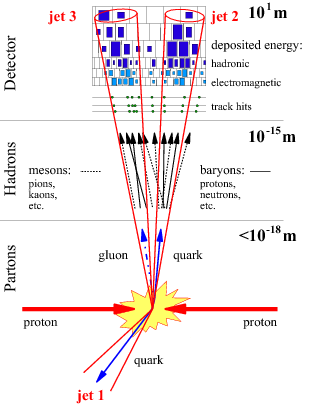
\includegraphics[width=0.4\linewidth]{Pics/cp4/41.png}
  	\caption{Illustration of jets at different scales. The jets can be characterized in three different stages, the so-called parton, hadron (particle) and detector level~\cite{Carli:2015qta}.}
   	\label{fig:41}
\end{figure}


\subsubsection{Jet reconstruction}
 For this analysis the jet reconstruction software FastJet 2.4.3~\cite{Cacciari:2011ma} is used to reconstruct jets formed at the electromagnetic (EM) scale from topological calorimeter cell clusters~\cite{Lampl:1099735}.  The anti-k$_T$ reconstruction algorithm~\cite{Cacciari:2008gp} is used with a radius parameter of $R$ = 0.4.
Calorimeter cells, where the deposited energy exceeds a certain noise threshold, are grouped to topological clusters. This noise threshold is obtained from measurements of the electronic noise of the calorimeter system and simulations of the pile-up noise~\cite{Aaboud:2017jcu}. 
 The clustering is performed by the anti-k$_T$ algorithm, which starts by calculating the distance of two distinguishable particles $i$ and $j$: 
\begin{equation}
d_{\rm i,j} = \text{min}(k_{\rm T,i}^{-2}, k_{\rm T,i}^{-2})\frac{(\Delta R_{\rm i,j})^2}{R^2}.
\end{equation}
$k_{\rm T,i}$ denotes the transverse momentum of the particle $i$, while $\Delta R_{\rm i,j}$ is the geometrical distance between the two particles in the detector coordinates (see~\cref{dinstance}).
The radius parameter $R$ determines  the size of the jet.
In addition to $d_{\rm i,j}$, the distance to the beam pipe $d_{\rm i,beam}=k_{T,i}^{-2}$ for each single particle is calculated. Those two parameters are compared, for the shortest distance. If $d_{\rm i,j}$ is smaller than $d_{\rm i,beam}$, the entities i and j are recombined. In the opposite case, i is referred to be a jet and removed. This procedure is repeated until all possible jet contributions are either absorbed into the jet candidate or removed.



\subsubsection{Jet energy scales}

 The reconstructed jets are built from calorimeter clusters obtained at a certain energy scale, determined by the deposited energy. The \textbf{jet energy scale (JES)} is calibrated in several consecutive steps derived from a combination of MC-based simulation and in-situ methods. The calorimeter jets are obtained at the \textbf{electromagnetic scale (EM)} and corrected in their orientation. Therefore, the four-momenta of the jets are orientated to point towards the primary vertex of the hard interaction, which results in an improvement of the $\eta$ resolution.  In the next calibration step, pile-up effects are removed, by the subtraction via the area-based $p_T$ method~\cite{Cacciari:2007fd} and  residual corrections are applied to the  jets in data.  The  average momentum contamination from pile-up is subtracted from each jet momentum, depending on the jet area $A$. The average $p_T$ per event density in the $\eta-\phi$ plane is calculated and for each jet taken to be $p_T/A$, using ghost particles. The measurement of the number of ghost particles  allows to determine the size of the  jet area $A$.~\cite{Aaboud:2017jcu}

 In order to reject jets originating from pile-up events,  additional cuts are applied. For jets with  $p_T <$ 60~GeV and within  0 $<\mid \eta \mid<$ 2.4,  a track-based technique is used, which rejects  jets from pile-up by the jet vertex tagger (JVT). Moreover, the effects of out-of-time pile-up are taken into account via the application of  a residual correction, which is derived from comparisons to truth particle jets in simulated dijet events.~\cite{Aad:2015ina}


 The calorimeter clusters are calibrated using the EM+JES calibration scheme, where the jet four-momenta are adapted to the particle-energy scale by the absolute JES calibration, which is derived as a correction of the energy of the reconstructed jets to the energy of simulated truth jets~\cite{Aad:2014bia}.
 In addition, the energy scale of the reconstructed jets is corrected with the information from the calorimeter, the MS and track-based variables.
  Within a distance of $\Delta R$, the simulated jets are geometrically assigned to isolated reconstructed jets. Isolated calorimeter jets have within a distance of $\Delta R$ = 0.6 no further calorimeter jet  and not more than one truth jet within a distance of $\Delta R$ = 1.0.  Here only calorimeter and truth jets with  $p_T$ > 7~GeV are considered. Corrections are applied with a residual in-situ calibration to correct jets in data using well-measured reference objects, e.g.  photons, $Z$-bosons and calibrated jets.~\cite{Aaboud:2017jcu}
 
 For the determination of the final jet energies at the  \textbf{EM+JES} scale, the simulated truth jets are matched to reconstructed calorimeter jets. 
 Furthermore,  the energy jet response 
$ R^{\rm jet}_{\rm EM}= E^{\rm jet}_{\rm EM} /E^{\rm jet}_{\rm EM}$,
  is evaluated for each matched pair. 
   $E^{\rm jet}_{\rm EM}$ denotes the energy of the observed calorimeter jets at the electromagnetic scale and $E^{\rm jet}_{\rm truth}$ the energy of the corresponding truth jets.  
    The response functions are used to derive $\eta$-dependent correction factors $F^{\rm jet}_{\rm cal}(E^{\rm jet}_{\rm EM})|_{\eta}$. The complete procedure is described in detail in~\cite{Aad:2011he}.
    With the obtained correction factors, the  jet energy at the EM+JES scale is determined:
    \begin{equation}
    E^{\rm jet}_{\rm EM+JES} = \frac{   E^{\rm jet}_{\rm EM}}{F^{\rm jet}_{\rm cal}(E^{\rm jet}_{\rm EM})|_{\eta}}. 
      \end{equation}
    
    
 An overlap removal is applied at the end, which prevents the double-counting of electrons as a jet. Therefore, the closest jet to an electron, within a cone of $\Delta R $ < 0.2, is removed. Furthermore, electrons in a cone $\Delta R $ < 0.4 around a jet are rejected. The same is done for muons, if the jet can be associated to at least three tracks, otherwise the jet is removed.
 
 
 At last, it should be mentioned that the JES depends on the flavours. 
 Particular jets assigned to $b$ quarks ($b$-jets) tend to have larger contributions from weak decays, which produce neutrinos, compared to jets from lighter quarks. These leads to an underestimation of the energy of the corresponding calorimeter jet. Therefore, an additional \textbf{$b$-to light jet energy scale (bJSE)} is considered.  The uncertainties related to the energy scale of $b$-jets is calculated as the sum in quadrature of the corresponding JES and bJES uncertainty.   

 



\subsection{Tagging of $b$-Jets}
In the measurement of the top-quark mass, the identification of jets originating from $b$-quarks is particularly important, since  top quarks almost exclusively decay into $b$-quarks and a $W$-boson (see~\cref{decay1}). This can be done using the fact that the hadrons containing a $b$-quark have a significant  lifetime, which results in a relatively large propagation of those so-called $B$-hadrons, until the decay. The  large distances which the particles travel in the detector allow to distinguish them from non-$B$-hadrons.   
The  jets  from $b$-quarks can thus be identified by the reconstruction of the $B$-hadron decay vertices, due to a noticeable shift of the  jet axis and a large impact parameter (see~\cref{fig:42}). These jets are referred in the following as $b$-jets, while jets associated with hadrons from lighter quarks, $u, d, s, c$ or gluons are called light jets.

On the one hand, $b-$tagging offers the huge advantage to improve the event selection by applying cuts on the number of tagged jets, thus reducing certain background contributions. On the other hand, it is a cornerstone for the kinematic reconstruction of the event, since it allows to distinguish the $b$-jets from the light jets of the $W$-boson decay. 

\begin{figure}[h]
	\centering
	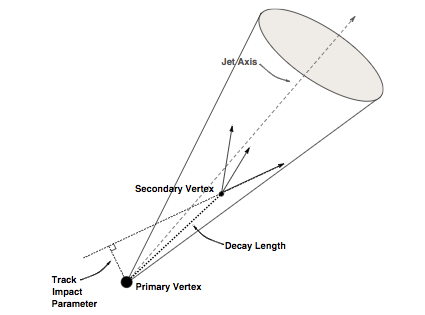
\includegraphics[width=0.5\linewidth]{Pics/btag.png}
	\caption{ Illustration of the $b$-jet reconstruction, with the characteristic decay length between the primary and secondary vertex ~\cite{ATLAS:2010rza}.} 
	\label{fig:42}
\end{figure}

The $b$-jet identification in this thesis is based on the MV2c10 method~\cite{ATL-PHYS-PUB-2016-012}, which combines the results of the three standard  $b$-tagging algorithms, which are taking the jet $p_T$ and the $\eta$ region into account.

 The first algorithm is the IP3D, which is a lifetime-based tagging method~\cite{ATL-PHYS-PUB-2016-012}. In addition, the inclusive multi-vertex finding algorithm JetFitter~\cite{Piacquadio:2008zza} is applied, followed by a secondary vertex reconstruction with the SV algorithm~\cite{ATLAS-CONF-2011-102}.

 The output of the three basic  tagging algorithms are combined with a Boosted Decision Tree (BDT)~\cite{ATL-PHYS-PUB-2016-012}. 
The information of the three algorithms is 
 used to calculate a discrimination weight $w$ within the multivariate analysis, which represents  the probability of a certain jet  to contain a $B$-hadron.  While for $b$-jets, this weight is close to unity, light jets can be associated to small values of $w$.


 
A $b$-tagging working point (WP) is chosen by constraining $w$ via specific cuts, to determine the efficiency of the tagging algorithm, i.e. the probability that a jet is correctly identified as $b$-jet. 
 Furthermore, a rejection factor is taken into account.  Here, the chosen working point belongs to an average $b$-tagging efficiency of 77~\%, obtained in simulated $t\bar{t}$ events. For jets referred to  $c$-hadrons, the rejection factor is 6.2, while for lighter flavoured  hadrons it is 134. 
 


\subsection{Missing transverse  energy}\label{ET}

The transverse energy ($E_T$)  is determined with the cell structure of the calorimeter system.  For a physical object, the transverse energy can be calculated with:
\begin{equation}
E_T = E \text{sin}(\theta).
\end{equation}
$E$ is the measured energy, which belongs to the corresponding calorimeter cells of the jet. The polar angle ($\Theta$)  provides the information  about the  direction of the jet with respect to the beam pipe. 

 

$E^{\rm miss}_T$ is defined as the negative vector sum of the transverse momentum $p_T$ of all selected physical objects. Furthermore, an additional so-called soft term is taken into account, considering disturbances like the false reconstruction of tracks.
A certain amount of missing transverse energy $E^{miss}_T$ ~\cite{ATL-PHYS-PUB-2015-027} can arise due to weakly interacting particles in the final state, e.g. the neutrino in the $t\bar{t}\rightarrow$ lepton + jets channel or from energy leakage effects in the detector.

 For the determination of $E^{miss}_T$, Monte Carlo simulation is compared to data of the year 2015, with a track-based soft term (TST) ~\cite{ATL-PHYS-PUB-2015-027}. The soft-term is reconstructed from Inner Detector tracks, which are associated with the primary vertex of the selected physical objects and provide  information about the non-selected contribution.  
The missing transverse energy is built per event.


 



\section{Data and Monte Carlo samples}\label{DATA}

This analysis is based on the data taken in 2016 with the ATLAS detector, obtained from  $pp$ collisions at a center-of-mass energy of $\sqrt{s}$= 13~TeV, with a corresponding luminosity of 33~fb$^{-1}$. For several purposes of this analysis, e.g. the simulation of the different signal and background contributions or the estimation of interactions with the detector material, Monte Carlo generators (MC) are used. 



The matrix elements (ME) of the signal $t\bar{t}$ samples are simulated at next-to-leading order (NLO), using the \textsc{Powheg-Box v2} generator%(r3026)
~\cite{Nason:2004rx,Frixione:2007vw,Alioli:2010xd}, with the \textsc{NNPDF 3.0} parton distribution function (PDF) ~\cite{Ball:2014uwa}. The parton shower is modelled in leading-order (LO) with \textsc{Pythia 6}~\cite{Sjostrand:2006za} in perturbative QCD, with the~\textsc{NNPDF 2.3} PDF~\cite{Ball:2012cx}  and the \textsc{Perugia 2012} tune~\cite{Skands:2010ak}.
The hadronization and  underlying events are also modelled  with the \textsc{Pythia 6} program. In addition, the nominal $t\bar{t}$ sample ($m_{\text{top} }$= 172.5~GeV)  is also produced with \textsc{Pythia 8}~\cite{Sjostrand:2007gs} , the same PDF sets and the A14 tune~\cite{ATL-PHYS-PUB-2014-021}.
The top-quark mass is assumed to be 172.5~GeV and the damping parameter $h_{\rm damp}$, which regulates the $p_T$ emissions beyond the Born parton shower (PS) configuration, is chosen to be 1.5~m$_{\rm top}$ for  \textsc{Powheg + Pythia 8} and 1.0~m$_{\rm top}$ for  \textsc{Powheg + Pythia 6}.


For the NLO matrix element of the single top events, the \textsc{Powheg-Box v1} generator with the \textsc{CT10} PDF~\cite{Lai:2010vv} is used. The parton shower is also simulated in LO with the  \textsc{Pythia 6} program, using the \textsc{CTEQ6L1}~\cite{Pumplin:2002vw} PDF and the \textsc{Perugia 2012C} tune.  The top-quark mass is assumed to be 172.5~GeV and there is no  $h_{\rm damp}$ for single top quarks.


  $W$- and $Z$-boson events with jets are modelled using the  \textsc{Sherpa 2.2.1} MC generator~\cite{Gleisberg:2008ta,Schumann:2007mg,Hoeche:2012yf}, which provides the matrix elements in  NLO.  The corresponding PDF is  \textsc{NNPDF 3.0}. \textsc{Sherpa} is also used for the simulation the ME and the PS of diboson processes ($WW$, $WZ$ and $ZZ$) in NLO, interfaced with the \textsc{CT10} PDF set. $t\bar{t}V$ processes are events with a top-quark pair and a $W$- or a $Z$-boson. The ME is calculated in NLO with the MG5\_aMC@NLO generator~\cite{Alwall:2014hca}, with \textsc{NNPDF 3.0} and  \textsc{Pythia 8} with~\textsc{NNPDF 2.3} and the \textsc{A14} tune.

 The impact of multi-$pp$ collisions is simulated for all samples by soft QCD processes with the \textsc{Pythia 8}  program. The applied parameter set is provided from the \textsc{A2} tune~\cite{ATL-PHYS-PUB-2012-003}, while the \textsc{MSTW2008LO} PDF ~\cite{Martin:2009iq} is taken.

 For mass hypotheses testing, $t\bar{t}$ samples are derived for different mass points, with $m_{\text{top}}$ = 170.0, 171.5, 172.5, 173.5 and 175. The signal MC samples are normalised for $m_{\text{top}}$ = 172.5~GeV to a cross-section of 832 $\pm$ 46~pb, calculated with the \textsc{Top++ 2.0} framework~\cite{Czakon:2011xx} in next-to-next-to-leading-order QCD and with 
the resummation of next-to-next-to-leading logarithmic soft gluon terms~\cite{Cacciari:2011hy,Beneke:2011mq,Baernreuther:2012ws,Czakon:2012zr,Czakon:2013goa}.  For the normalization of the background samples, the corresponding  theoretical cross-sections are calculated in at least NLO  QCD~\cite{Catani:2009sm,Kidonakis:2010tc,Kidonakis:2010ux,Kidonakis:2011wy,Campbell:1999ah,Campbell:2011bn,Alwall:2014hca,deFlorian:2016spz,ATL-PHYS-PUB-2016-003}. 
 



 In order to consider the  interactions with the detector material, each simulated sample has to undergo the ATLAS detector and trigger simulation~\cite{Aad:2010ah}. Therefore, \textsc{Geant 4}~\cite{Agostinelli:2002hh}  is used to simulate the interactions with the detector components.  In addition, for the evaluation of systematic uncertainties, signal MC samples are produced with the much faster \textbf{Atlfast 2.0}~\cite{Richter-Was:683751} simulation. This method leaves the simulation of the inner detector system unchanged, while using a faster approximation for the energy deposition in the calorimeter system.

 In addition to the samples produced for the data/MC comparison further samples are needed for the evaluation of the systematic uncertainties. More details can be found in~\cref{sec:Uns}. 



\section{Event preselection and background contributions}\label{selection}
 One of the most difficult tasks at modern hadron collider experiments is the handling of the large amount of data and the selection of the interesting physical processes. Therefore, analysis dependent quality criteria are applied, taking the characteristic event topology of the  $t\bar{t}\rightarrow$ lepton + jets into account. In addition, the chosen selection cuts try to minimize the background contamination of the signal region. 
 
 In the following, the different background contributions for the lepton + jets channel will be discussed, before the applied event triggers and selection cuts are presented together with the control distributions of the observables.
 
 \begin{figure}[h]
 	\centering
 	\includegraphics[width=1.0\linewidth]{background.png}
 	\caption{Leading-order diagrams of the main background processes, which affect the measurement of the top-quark mass in the lepton + jets channel.  The letters in brackets mark possible miss interpretations of gluons. In the case of the  second diagram, the differences of the $W$+jets and $Z$+jets are marked blue. } 
 	\label{fig:43}
 \end{figure}
 
 
 \subsection{Single top background}
 
 In the phase space of the $t\bar{t} \rightarrow$lepton + jets decay, several background processes contribute to the measurement. The main background processes are displayed in ~\cref{fig:43}.  Those background events are able to pass certain selection criteria and can be misidentified as signal events.
 
 Single-top events, like ~\cref{fig:43} (a), are a major background process, due to the presence of the top-quarks. They can lead to a simultaneous event structure and  event kinematic as of the lepton + jets  decay channel. A reason for the mis-matching can for example be the mis-identification of a gluon as a $b$ quark.
 However, there is a noticeable mass dependence of single-top events, which is the reason why it has been added to the signal region in the previous analyses~\cite{ATLAS-CONF-2017-071, Aad:2015nba}. Nevertheless, in terms of this thesis, single top events are referred to as background, due to missing MC samples for the different mass points\footnote{Only the nominal sample for 172.5~GeV is available for single-top production.}. 
 
 \subsection{Diboson background}
 The top-quark mass measurement is also affected by final states with two $W$-bosons, two $Z$-bosons or the combination of a $W$- and a $Z$-boson.  If one of the two bosons decays leptonically, while the other one decays into hadrons, this can lead to the mis-identification with the detector signature of the lepton + jets final state.  
 

 \subsection{$W$ + jets background}
The main background source  are $W$ + jets events (see~\cref{fig:43} (b)). This event type arises from $W$-boson production together with strongly interacting particles (quarks and gluons), which end up as additional jets. Particular events, where the $W$-boson decays leptonically, can lead to detector signatures, which can easily be mis-identified with $t\bar{t} \rightarrow$ lepton + jets events.



 \subsection{$Z$ + jets background} 
In addition to the $W$ + jets background, there are also events with a leptonically decaying $Z$-boson which, together with hadronically decaying particles, have a similar detector signature as the  $t\bar{t} \rightarrow$ lepton + jets final state. (see~\cref{fig:43} (b)). As shown in the following, the $Z$ + jets background is about one magnitude smaller than the $W$ + jets background and can be easily suppressed by requesting exactly one charged lepton and $b$-jets.



\subsection{Multijet/non-prompt lepton background}
QCD-multijet events are final states which do not contain any primary leptons (see~\cref{fig:43} (c)). They only arise from hard-scattering processes of strongly interacting particles (quarks and gluons). However, some hadronic jets can be misidentified as electrons, due to the energy deposition in the Electromagnetic Calorimeter. One refers to these jets as fake-lepton background. Furthermore, weak hadron decays inside of an hadronic jet lead to the identification of further leptons, which might be able to pass the isolation criteria (non-prompt leptons).
The consideration of the non-prompt/fake lepton background is very important, due to the fact that this contribution can be mis-identified with the charged isolated leptons arising from the $W$-boson decay of the $t\bar{t}$ final state.

The QCD-multijet  background has not been estimated yet and will not be included in this thesis.
 
 

 \subsection{Event triggering}

 

 \begin{center}
 	\captionof{table}{Trigger setup for electrons and muons. }\label{tab:trigr2}
 	
 	
 	
 	\vspace{0.3cm}	
 	
 	
 	\begin{tabular}{>{}m{7.0cm}>{}m{3.0cm}>{}m{3.0cm}} \toprule
 			Trigger&  lepton&$p_T$ cut /[GeV]\\
 			\midrule
 		
 		HLT\_e26\_lhtight\_nod0\_ivarloose& electron&  26\\
 		HLT\_e60\_lhmedium\_nod0  & electron&  60 \\
 		HLT\_e140\_lhloose\_nod0& electron &140\\
		HLT\_mu26\_ivarmedium & muon & 26\\
		HLT\_mu50 & muon & 50\\
 	

 		
 		\bottomrule
 	\end{tabular}
 	
 \end{center}
\clearpage
  In context of this measurement, events containing single leptons (electrons and muons) are selected using different single lepton triggers.
 For each case of the $t\bar{t} \rightarrow$ lepton + jets decay, several  trigger options for the single leptons are available, which do not take any further hadron information into account. The used trigger setup is given in~\cref{tab:trigr2}.
 
 
 
 
 
 
 
\subsection{Preselection criteria} 
In order to obtain the $t\bar{t} \rightarrow$ lepton + jets events and perform an efficient separation from background, one uses the fact that each of the interesting events can be identified by its characteristic decay topology, with  two $b$-jets and at least two light jets. Furthermore, the detector signature contains one charged isolated lepton and the corresponding neutrino, which can only be registered by considering the missing transverse energy $E^{miss}_T$. Preselection cuts are applied to obtain events with these criteria using a similar selection as for the previous analyses for 7~TeV~\cite{Aad:2015nba} and 8~TeV~\cite{ATLAS-CONF-2017-071}:




\begin{itemize}
	\item  At least one good primary vertex has to be obtained for selected events\footnote{The primary vertex is the one  with the highest   $\sum p_T^2$, where  $p_T$ denotes the transverse momentum and the sum runs over all associated  tracks.}.
	\item In addition the single-electron or single-muon  trigger has to have fired.
	\item The triggered leptons are further required to have a transverse energy of $E_T > $ 27~GeV for electrons, while for muons, the transverse momentum $p_T$  must exceed 27~GeV. 
	\item For the electron + jets channel, additional cuts are applied:  $E_T^{\rm miss}$ > 30~GeV,  $m_T^W$ > 30~GeV\footnote{The transverse $W$ mass is defined as: $m_T^W$ =$\sqrt{2p_T^lE_T^{\rm miss}(1-cos\phi(l,E^{\rm miss}_T))}$, where $l$ denotes the charged lepton.} and $E_T^{miss} + m_T^{W} > 60$~GeV.
	\item Events with a muon are required to have a missing transverse energy of at least
	20~GeV  and to fulfil the relation: $E_T^{\rm miss} + m_T^{W} > 60$~GeV.
	\item Furthermore, events are only selected if they contain at least four jets, with a $p_T$ above 25~GeV in the central region of the detector ($\mid \eta \mid $ < 2.5).
	\item At least one of the jets  has to be tagged as a $b$-jet. 
\end{itemize}

 In addition to the preselection cuts there are analysis specific cuts on some global quantities in analogy to~\cite{ATLAS-CONF-2017-071}. These quantities, e.g. the reconstructed top-quark mass, are obtained  from the event reconstruction and will be discussed in detail in~\cref{ch5}, together with the results of the preselection.





















\clearpage

\chapter{Event reconstruction}\label{ch5}
The second step of the analysis, following the event selection, is the event reconstruction, where the $t\bar{t}$ final-state is rebuilt by the selected information from its decay products. Therefore, the reconstructed jets have to be assigned to the initial partons, taking the event topology and kinematics into account. For this reconstruction, the same approach as for the previous measurements~\cite{Aad:2015nba, ATLAS-CONF-2017-071} is used, based on a kinematic maximum likelihood fit. 

The details of the reconstruction are introduced in this section, before the results and the control distributions of the reconstructed observables are discussed.  


\section{Reconstruction of the $t\bar{t}$ final-state}
\begin{figure}[h]
	\centering
	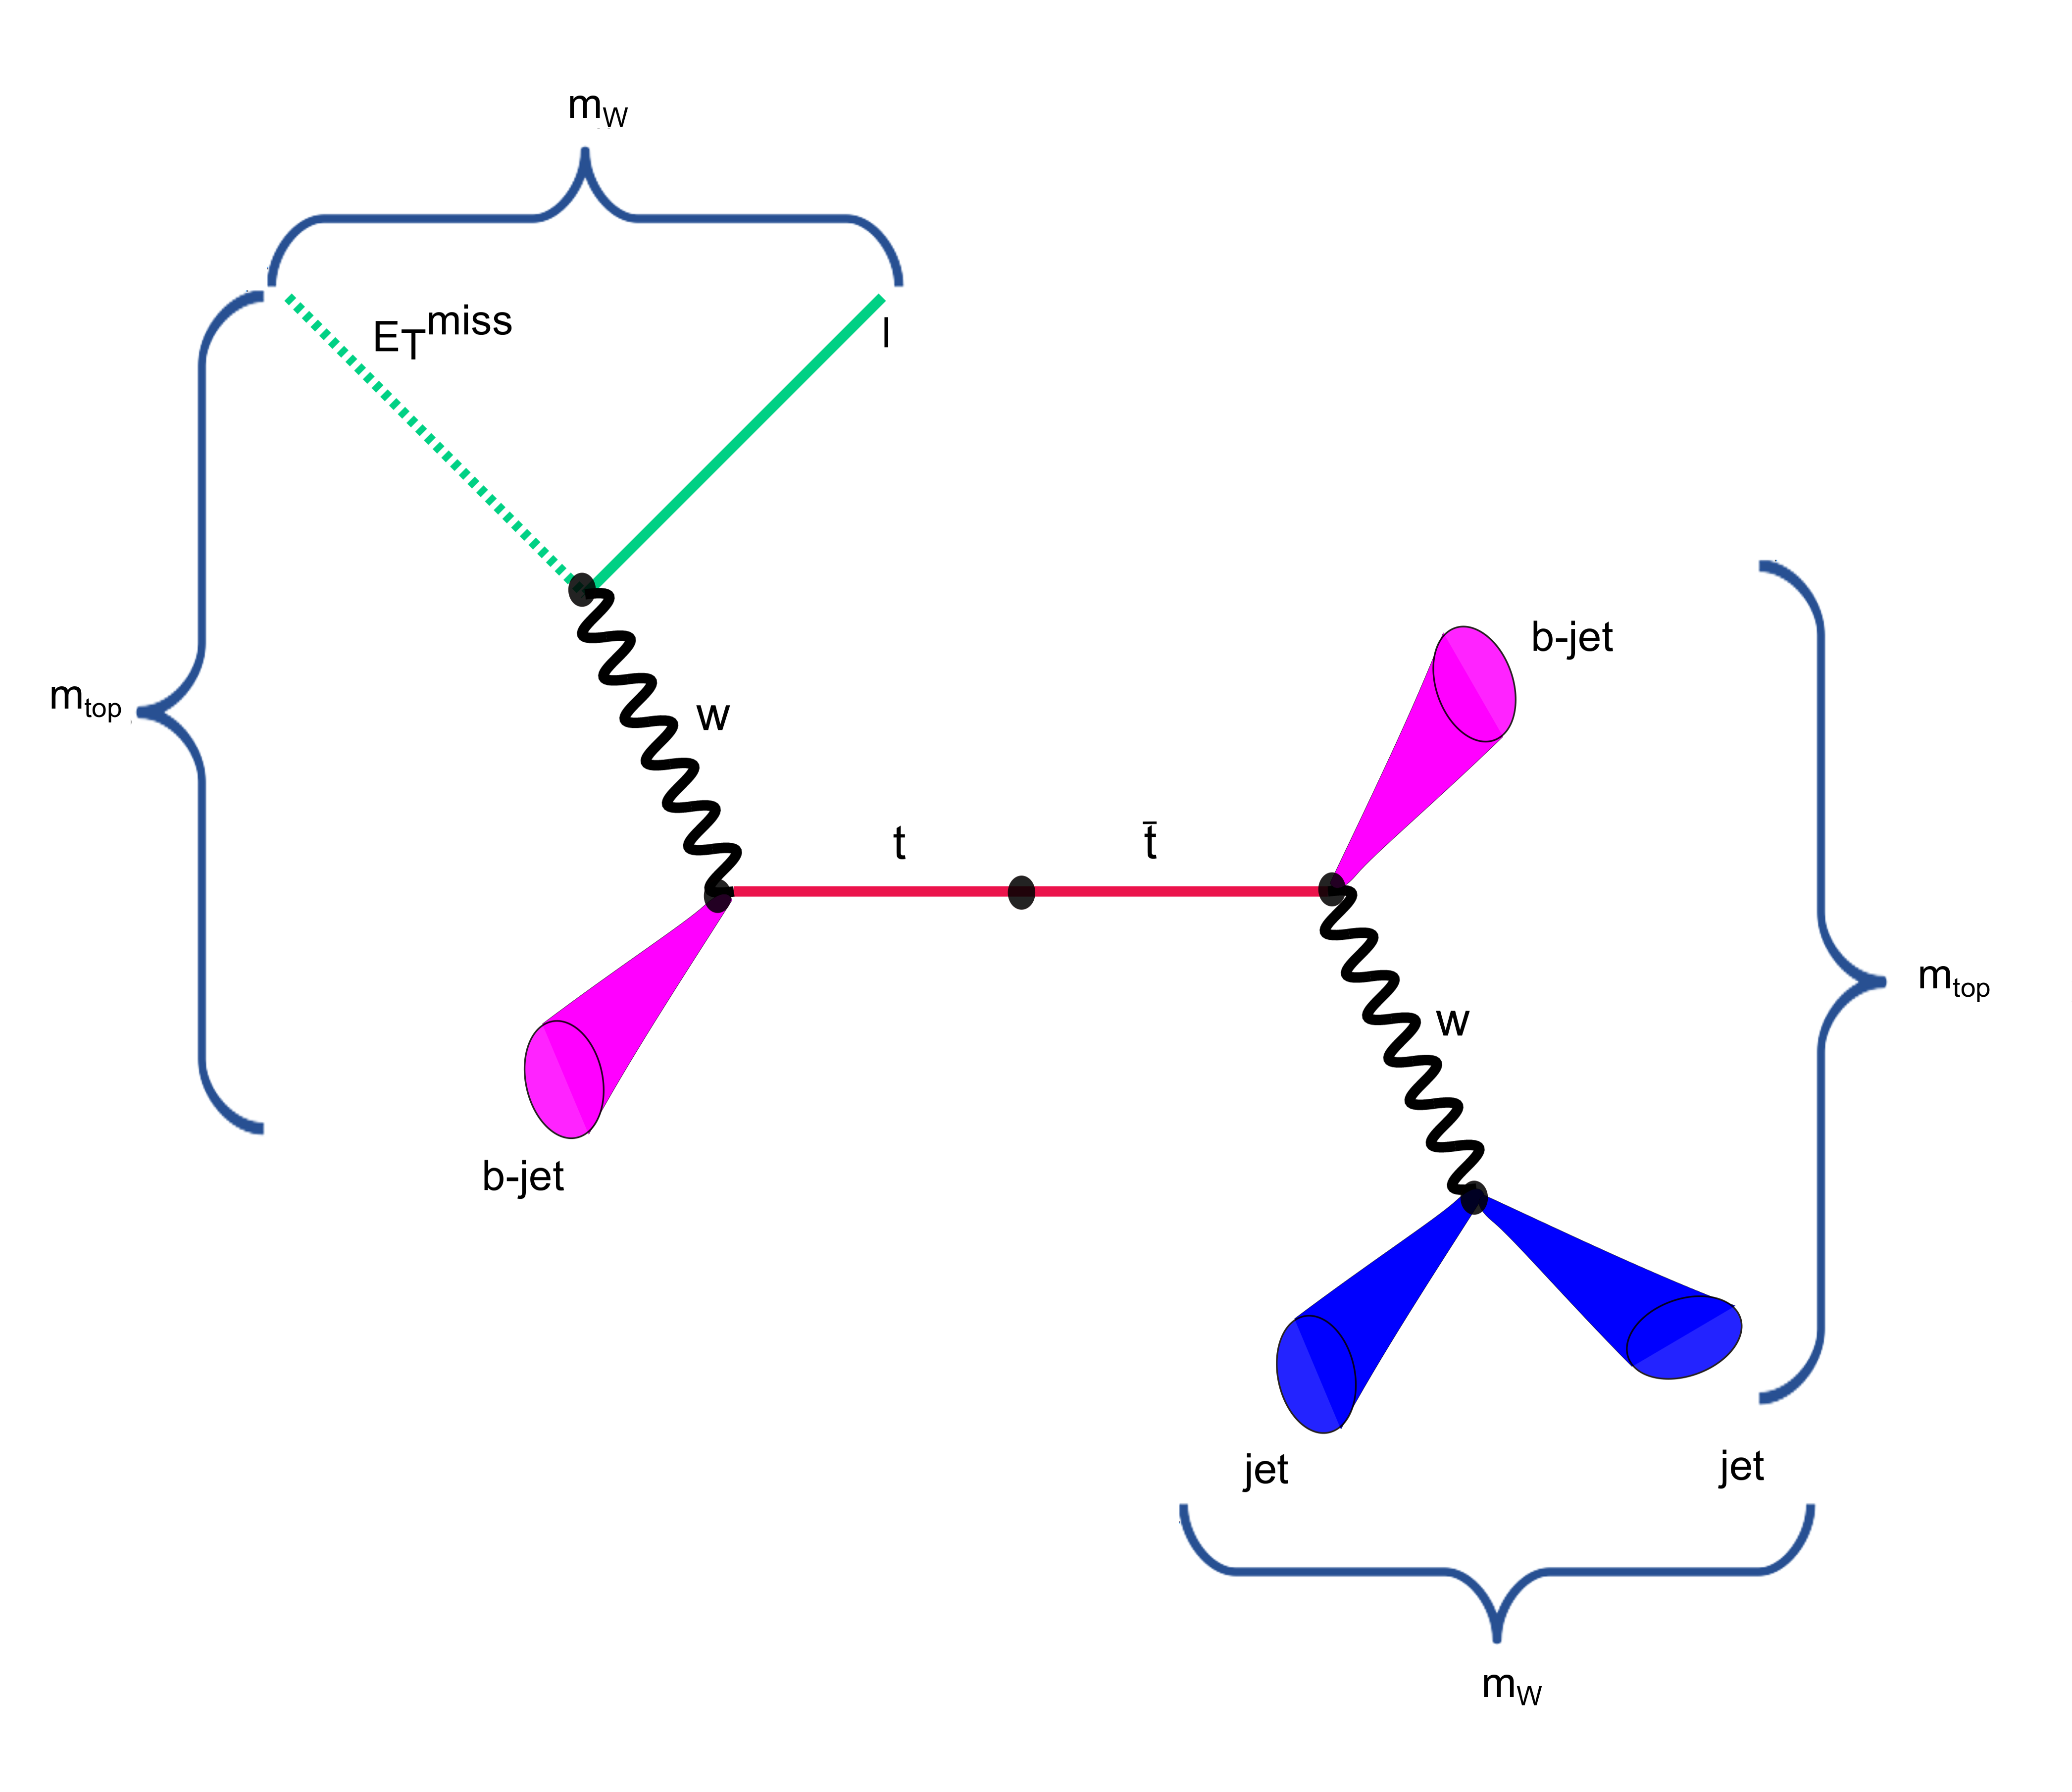
\includegraphics[width=0.65\linewidth]{Pics/cp5/51}
	\caption{ Illustration of the reconstruction of the $t\bar{t}$ final-state. The  invariant masses of the hadronically and leptonically decaying top-quark are shown, as well as the corresponding $W$-boson masses. } 
	\label{fig:51}
\end{figure}

As displayed in~\cref{fig:51}, events with at least four jets are selected in this analysis. Therefore, one ends up with 4! = 24 possible jet-parton assignments, which will be denoted as permutations in the following. The minimum number of permutations gets further reduced by not distinguishing between the light jets of the $W$-boson decay, resulting in a total of 12 permutations. 

In order to find the best jet-parton assignment, a kinematic likelihood fit is performed with the \textsc{KLFitter} framework~\cite{Erdmann:2013rxa}. Within this program, the best possible jet-parton matching is evaluated based on the leading-order kinematics of the $t\bar{t}$ decay. For each permutation of the jets, a kinematic likelihood function ($L_{ \textsc{KLFitter}}$) is defined, using reconstructed properties like the hadronic $W$-boson mass, which is the invariant mass of the two jets of the hadronic top-quark decay $m(q_1q_2)$.

In the following, $q_1, q_2$ denote the light quarks of the $W$-boson decays, where $b_{had}$  is referred to  the $b$-quark from the hadronic top-quark decay and $b_{lep}$ to the leptonic one.  $E_{jet_i}$ is the energy of the jet number $i$. Properties of the charged lepton are labelled with $l$, while $\nu$ refers to the neutrino. All masses shown in~\cref{fig:51} are calculated and related to the  predicted kinematics for the leptons and the quarks of the $t\bar{t}$ decay.


The input variables for the kinematic likelihood fit are the four momentum of the charged lepton $E_{l_i}$, the $y$ and $x$ components of the missing transverse momentum ($p_{\nu,x}$, $p_{\nu,y})$ and the four momenta of the jets.
If the event contains more than four jets, the reconstruction efficiency can be increased by allowing more jets as input to  \textsc{KLFitter}. As shown in~\cite{ATLAS-CONF-2017-071} using up to six jets is beneficial for the event reconstruction. 
For events with at least two $b$-jets, the two highest $p_T$ $b$-tagged jets and the two highest $p_T$ untagged jets are used. Furthermore, the so-called veto mode is applied to improve the reconstruction efficiency and to reduce the number of possible permutations. This mode does not allow to assign a $b$-jet at the position of a light jet and vice versa. 

The kinematic likelihood function is given by eq.~(\ref{eq:Likeklf}) and consists of products of Breit-Wigner distributions ($BW$) and transfer functions ($T$).
The $BW$ distributions are based on a leading-order picture, where all jets are matched with the corresponding parton and the pole masses of the top-quarks~\cite{Erdmann:2013rxa}. 
Therefore, the $BW$ distributions are calculated for the input momenta of the quarks and leptons, with the corresponding invariant masses and the transverse momentum of the neutrino. 
The first term in the brackets of the $BW$ shows the invariant masses, which are reconstructed with \textsc{KLFitter}. These are the two jet mass $m(q_1q_2)$, the mass of the lepton pair $m(l \nu)$, the invariant mass of the hadroniclly decaying top quark $m(q_1q_2 b_{had})$ and the  invariant mass of the leptonic decaying top quark $m(q_1q_2 b_{lep})$. In addition,  $m_W$  and the corresponding width $\Gamma_{\text{W}}$ are taken into account, as well as the top-quark width $\Gamma_{\textsc{top}}$.
The reconstructed top quark mass $m_{\text{top}}^{\rm reco}$ is a free parameter in the kinematic likelihood fit. The mass parameter of the $W$-boson is set to the official particle data group  result around 80.39 $\pm$ 0.015~GeV~\cite{Olive:2016xmw}. 

\begin{eqnarray}
\label{eq:Likeklf}
L_{KLFitter} &=& 
BW[m(q_1q_2)|m_{\rm W},\Gamma_{\rm W}]\cdot BW[m(l \nu)|m_{\rm W},\Gamma_{\rm W}]\cdot\ \nonumber\\
&&BW[m(q_1q_2 b_{had})| m_{\text{top}}^{\rm reco},\Gamma_{\rm top}]\cdot BW[m(l \nu b_{ lep})|m_{\text{top}}^{\rm reco},\Gamma_{\rm top}]\cdot \nonumber \\
&&T(E_{jet_1}|\hat{E}_{b_{had}})\cdot T(E_{jet_2}|\hat{E}_{b_{lep}})\cdot \nonumber \\ 
&&T(E_{jet_3}|\hat{E}_{q_1})\cdot T(E_{jet_4}|\hat{E}_{q_2})\cdot \nonumber \\
&&T(E_{x}^{miss}|\hat{p}_{x,\nu})\cdot T(E_{y}^{ miss}|\hat{p}_{y,\nu})\cdot \nonumber\\ &&T(E_{y}^{miss}|\hat{p}_{y,\nu}) \cdot 
\left\{\begin{array}{II}
T(E_{e}|\hat{E_e}) \hspace{0.5cm} \text{ $e$ + jets}\\

T(p_{T_{\mu}}|\hat{p}_{T_{\mu}}) \hspace{0.5cm} \text{ $\mu$ + jets}\\
\end{array}
\right\} \cdot W_{btag}\phantom{L =aaaaaaaa } 
\end{eqnarray}
The transfer functions represent the detector response and further disturbances, by describing the resolution of the reconstructed energies. Therefore, they take the jet energies $E_jet_i$ ($i$ = 1,2,3,4)  into account. The  term in the brackets denote the energies of the corresponding jets. Quantities in the likelihood, with a hat, belong to parton-level. Furthermore, there are transfer functions, which include the missing transvers energy by using  the corresponding components of the transverse momentum, e.g. $T(E_{x}^{miss}|\hat{p}_{x,\nu})$. As shown in e.q.~(\ref{eq:Likeklf}), different functions for muon and electron events are used. While for electrons the energy is taken into account for muons the transverse momentum is considered. Due to the changes which arise with the increasing center-of-mass energy, e.g. the different background evolution with $\sqrt{s}$, the transfer functions have to be obtained specifically for the conditions of the measurement. However, within the time scale of this thesis, the corresponding transfer functions for $\sqrt{s}=$13~TeV were not available. Therefore, the same transfer functions as for 8~TeV are used~\cite{ATLAS-CONF-2017-071}. The calculated transfer functions have a double gaussian from:
\begin{equation}\label{transfer}
T(E_{\rm Truth},E_{\rm reco}) = \frac{1}{2\pi(p_2 + p_3p_5)}
\begin{pmatrix}
e^{\frac{(\Delta E- p_1)^2}{2p_2^2}} + p_3e^{\frac{(\Delta E- p_4)^2}{2p_5^2}} 
\end{pmatrix}
\end{equation} 
The motivation for the double gaussian from is  the energy resolution of the detector.
This functional from describes the spectrum of the relative difference of the parton-level energy $E_{Truth}$ and the reconstructed Energy $E_{\rm reco}$:
\begin{equation}
\Delta E = \frac{E_{\rm Truth}-E_{\rm reco}}{E_{\rm Truth}}.
\end{equation}
At last, $b$-tagging weighting factor $W_{btag}$ is applied, which is 1 if the $b$-tagged jets and the untagged jets are in the correct position, and 0 otherwise. 





For this analysis, the object reconstruction is very important, because it provides the estimators, which are sensitive to the top-quark mass and are used for the measurement. The first estimator is the reconstructed top-quark mass $m_{\text{top}}^{\rm reco}$, which is a free parameter in \textsc{KLFitter} and contains improvement by a implicit constraint in the fit to the known $W$-boson mass.
Furthermore, two observables sensitive to the jet energy calibration are calculated for the chosen jet permutation, but from the original four momenta. These are the reconstructed $W$-boson mass $m_\text{W}^{\rm reco}$, which is related to the four momenta of the jets of the hadronically decaying top-quark. The second one is called $R_{\text{bq}}^{\rm reco}$, which is sensitive to the energy calibration of the $b$-jets and thus has two different definitions, for one- and two $b$-tags:
\begin{equation}
R^{\rm reco,1b}_{\rm bq} = \frac{2 p_T^{\rm b_{tag}}}{(p_T^{\rm W_{jet_1}}+p_T^{\rm W_{jet_2}})}
\hspace{0.5cm}
\text{and}
\hspace{0.5cm}
R^{\rm reco,2b}_{\text{bq}} = \frac{p_T^{\rm b_{had}}+ p_T^{\rm b_{lep}}}{(p_T^{\rm W_{jet_1}}+p_T^{\rm W_{jet_2}})}.
\end{equation}


In terms of this analysis, only events with at least two $b$-jets are used for the reconstruction. Thus, only the second definition for  $R_{\text{bq}}^{\rm reco,2b}$ is used here and just called $R_{\text{bq}}^{\rm reco}$ in the following. Furthermore, all three reconstructed variables are constrained by cuts, which are implemented before the event reconstruction:  $m_{\text{top}}^{\rm reco}  \subseteq [125,200]$~GeV,  $m_{\text{W}}^{\rm reco}  \subseteq [55,110]$~GeV and $R_{\text{bq}}^{\rm reco}  \subseteq [0.3,3.0]$. Moreover, events where the minimization of  \textsc{KLFitter} does not converge, are rejected. 


These cuts are applied on top of the cuts of the preselection. The corresponding event yields are displayed in~\cref{tab:T41}, for events with at least four jets, where at least two of them have to be tagged as $b$-jets. The total number of data events is shown, as well as the corresponding signal and background contributions. Furthermore, the event yields for the samples with four jets and at least one $b$-tag, are displayed in comparison. For the data-simulation comparison the top-mass is assumed to be 172.5~GeV. If not mentioned differently, all results just include statistical uncertainties and no uncertainties are considered for the data.

\vspace{0.5cm}
\begin{center}\
\captionof{table}{The observed number of events for a center-of-mass energy of 13~TeV and an integrated luminosity of 33~fb$^{-1}$. The event yields are presented for events with at least four jets with at least two $b$-tagged jets. Furthermore, the number of signal and background events for the nominal sample of $m_{\rm top} =$ 172.5~GeV are shown. The simulated results correspond to the  luminosity of the data. The statitical uncertainties are rounded to two significant digits.}\label{tab:T41}


	
\vspace{0.3cm}	
	

\begin{tabular}{>{}m{4.0cm}>{}m{3.0cm} >{}m{3.0cm}} \toprule

Process (Simulation)&   2 $b$-tags&  1 $b$-tags\\
\midrule
$t\bar{t}$ & 389550 $\pm$ 390& 720620$\pm$  520\\
Single top & 12909 $\pm$  66&36070 $\pm$  110\\
$W$+jets & 8000 $\pm$  410&79510 $\pm$  990\\
$Z$+jets & 1810 $\pm$  90&13300 $\pm$  260\\
Diboson & 387.5 $\pm$  8.7&2957 $\pm$  28\\
$t\bar{t}+V$ & 18.17$\pm$  0.31&27.72 $\pm$  0.39\\
\midrule
Total signal + background & 412670 $\pm$  580&852500 $\pm$  1200\\
\midrule
Data & 475166 &  998651\\
\midrule
Data/Prediction  &1.15 $\pm$ 0.0016 & 1.17 $\pm$ 0.0016\\

\bottomrule
\end{tabular}

\end{center}












\vspace{1.0cm}

In~\cref{tab:T41}, the shown single top events are treated as an additional background process.
The main background stems from $W$ + jets events. For the sample with at least two $b$-tags it is  2~\% of the total background and for the sample with one at least one $b$-tag is its 9~\%. However, the QCD-multijet background has not be estimated yet and might lead to noticeable contributions for the future analysis. The other background sources, e.g.  diboson  and $Z$ + jet events, play only a minor role. 

The choice of the selection cuts on events with at least two $b$-tagged jets, can be explained by the nature of the top-quark pair decay, which almost always produces two $b$-quarks.  As shown here, as well as by the previous measurements, the main background sources can be reduced impressively by the cuts on the number of tagged jets. In case of this analysis, the total background gets reduced from  15~\% towards 6~\% for events with two  $b$-tags. While this remarkable reduction leads to a noticeable decrease of the background, the predicted number of events remain consistent with the observed number in data. Based on this experiences, the selection cuts on events with at least four jets, where at least two have to be tagged as $b$-jets are used for this analysis.



Despite the fact that the three measurements at 7, 8 and 13~TeV are sharing the same main background sources, the relative contributions are different for each center-of-mass energy. This can be explained by the fact that the cross-sections of the different background sources depend differently  on the increasing center-of-mass energy.


\subsubsection{Global Quantities of the Preselection}

In~\cref{fig:Sel1,fig:Sel2,fig:Sel4}, chosen distributions of observables are displayed for events with at least two $b$-tagged jets, together with the data-simulation comparison ratio. These control plots correspond to the  2016 ATLAS data set, obtained at 13~TeV with a corresponding integrated luminosity of 33~fb$^{-1}$. The different backgrounds are also shown by the coloured histograms. If not mentioned otherwise, all shown distributions contain only the statistical uncertainties and the  predicted distributions are normalised to the observed number of events in data, due to the sensitivity of the top-quark mass on the distribution shape~\cite{ATLAS-CONF-2017-071}. Therefore, the \textsc{Powheg} + \textsc{Pythia 6} samples are used.

In general more data than events in  simulation can be seen, which seems to be constituent for all observables. Furthermore a slight offset, of the data points to the simulation can be observed in the normalization of several distributions.    
Here one as to keep in mind, that the QCD background is missing, as well as the systematic uncertainties.

Nevertheless, one has to mention, that there is one deviation from the good trend in the data-simulation comparison. For the third bin of the number of tagged jets~\cref{fig:Sec2}, a huge disagreement can be seen.

The displayed control distributions test also the quality of the Monte Carlo simulation.
Disagreements in the data-prediction comparison can for example  arise due to imperfections in the  modelling  with different physics generators. Furthermore, disagreements can appear if the \textsc{Geant4} simulation of the detector is not good enough. Therefore, the improvement of the simulation is one of the key tasks for the general physics analysis. 
The control distributions for the reconstructed quantities, are shown after the global quantities of the preselection.



\begin{figure} [b]% "[t!]" placement specifier just for this example
	\centering
\begin{subfigure}{0.25\textwidth}
	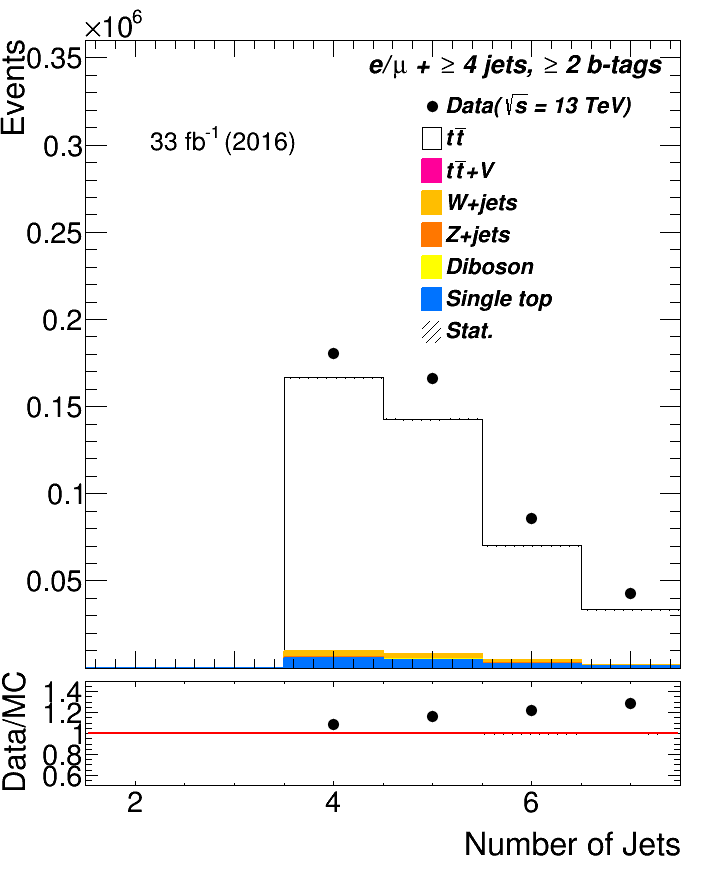
\includegraphics[width=\linewidth]{ControlPlots_emujets_2016_4incl_2incl/jet_n_emujets_2016.png}
	\caption{Number of jets.} \label{fig:Sec1}
\end{subfigure}
\hspace*{0.5cm}
\begin{subfigure}{0.25\textwidth}
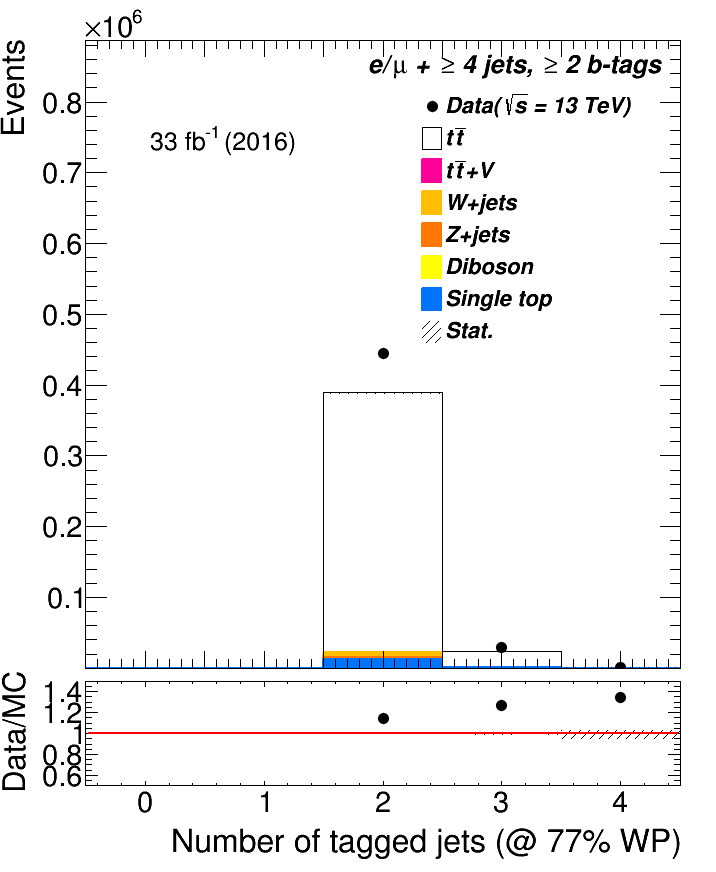
\includegraphics[width=\linewidth]{ControlPlots_emujets_2016_4incl_2incl/nBTags_emujets_2016.png}
\caption{Number of $b$-tagged jets.} \label{fig:Sec2}
\end{subfigure}
\hspace*{0.5cm}
\begin{subfigure}{0.25\textwidth}
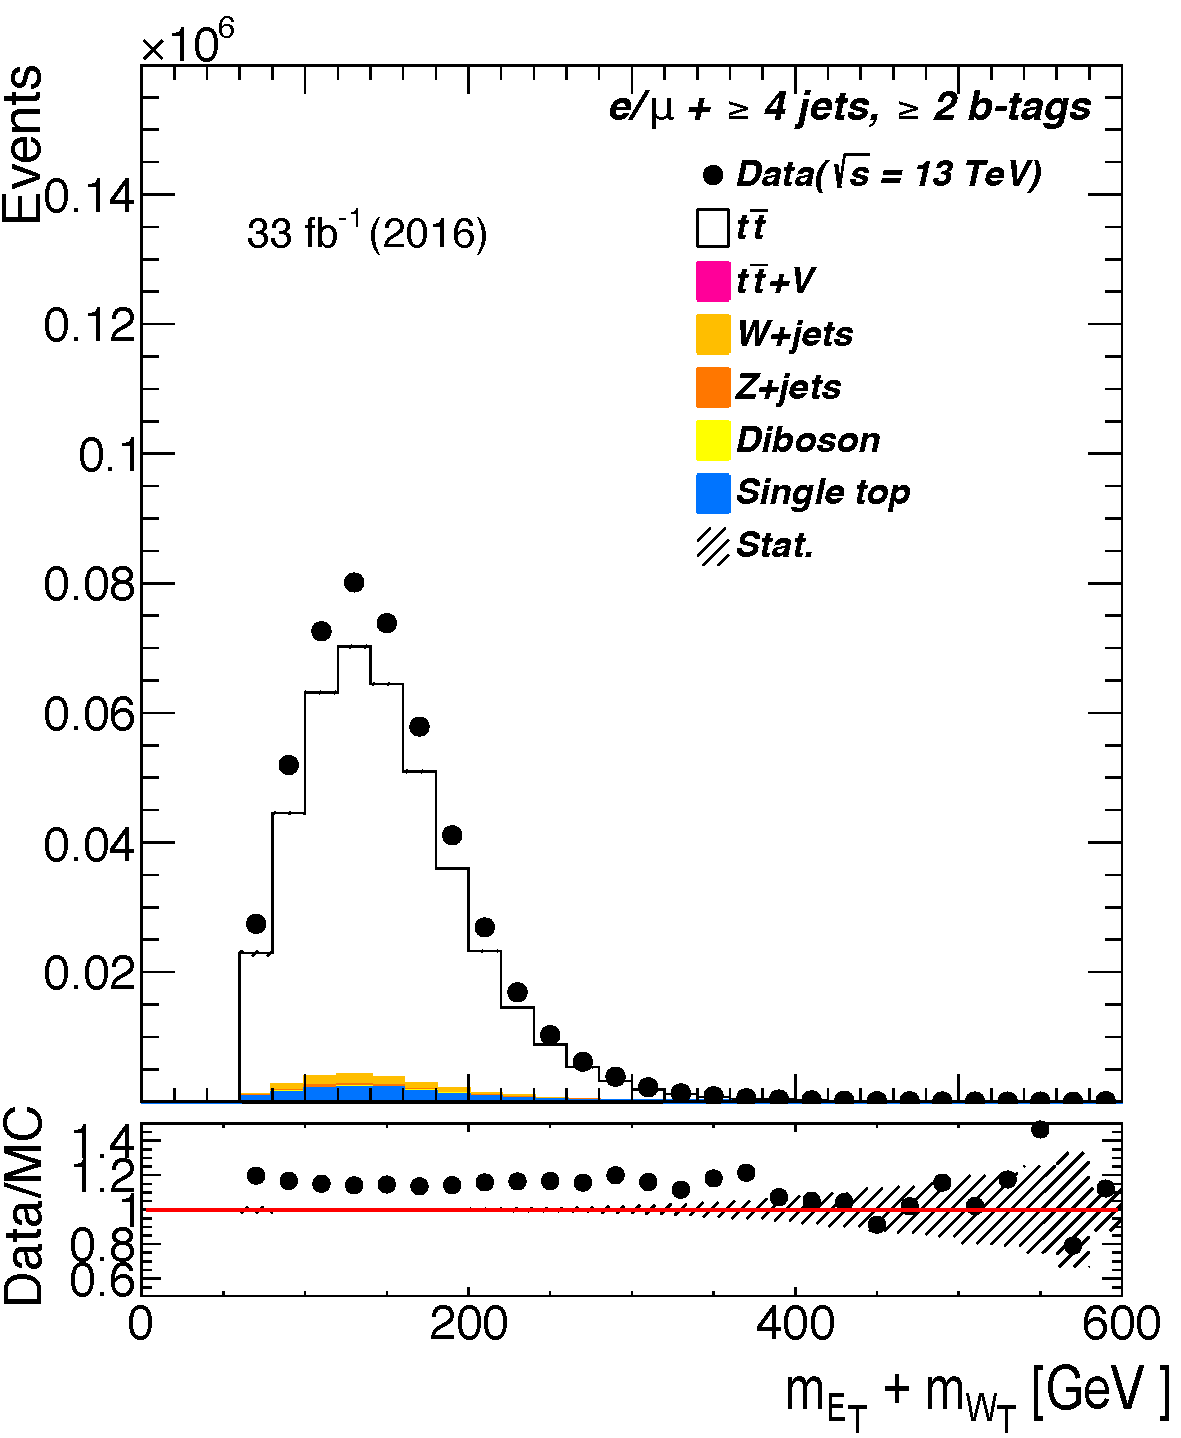
\includegraphics[width=\linewidth]{ControlPlots_emujets_2016_4incl_2incl/met_plus_mtw_emujets_2016.pdf}
\caption{$E_T^{miss}$ + $W_T$-mass.} \label{fig:Sec3}
\end{subfigure}
	
	
\begin{subfigure}{0.25\textwidth}
	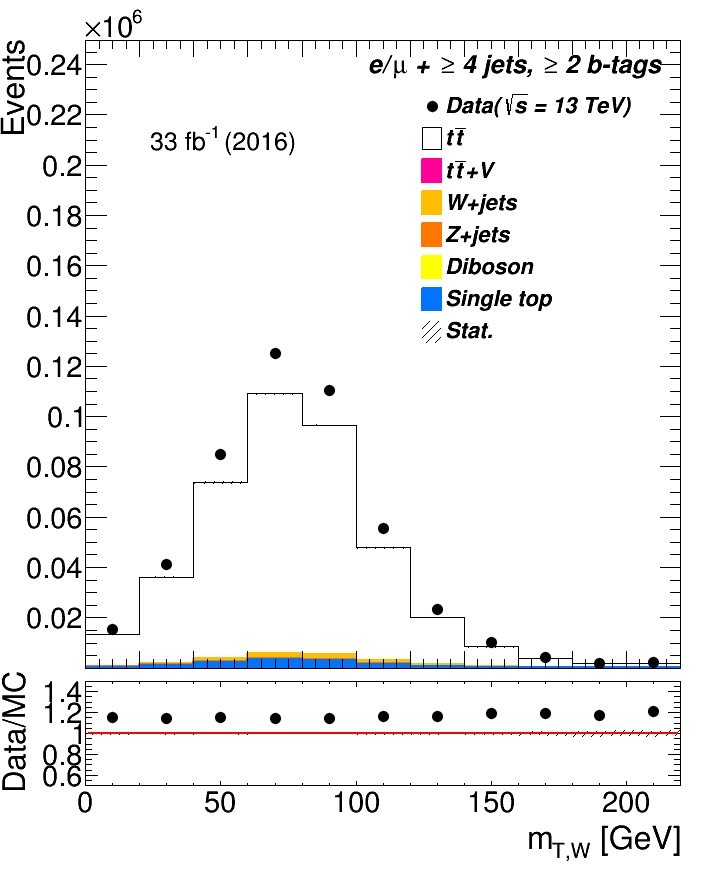
\includegraphics[width=\linewidth]{ControlPlots_emujets_2016_4incl_2incl/mtw_emujets_2016.png}
	\caption{Leptonic  $W_T$-mass.} \label{fig:Sec4}
\end{subfigure}
\hspace*{0.5cm}
\begin{subfigure}{0.25\textwidth}		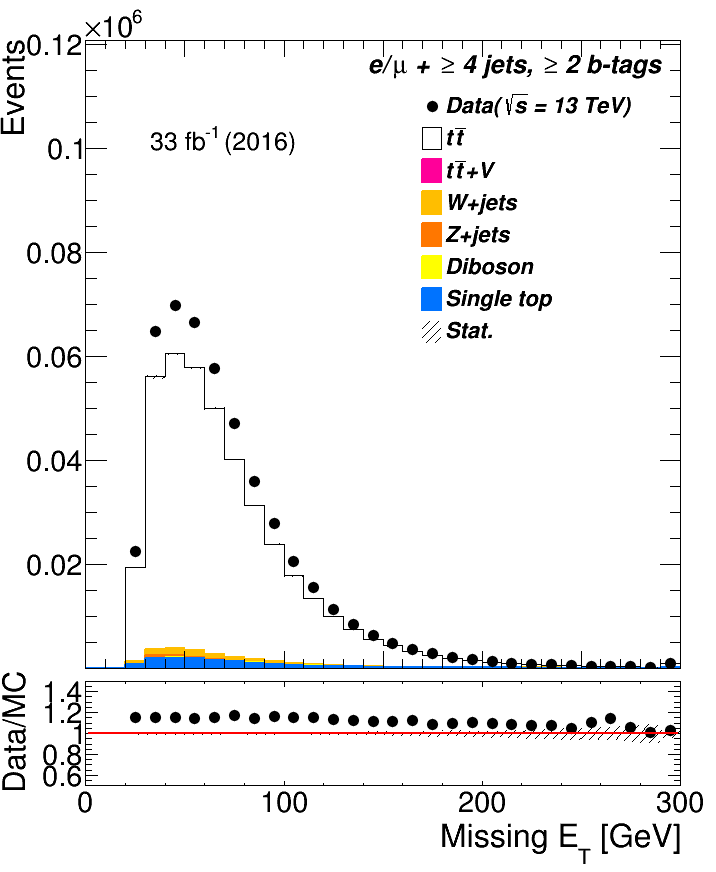
\includegraphics[width=\linewidth]{ControlPlots_emujets_2016_4incl_2incl/met_met_emujets_2016.png}
	 	\caption{$E_T^{miss}$.} \label{fig:Sec5}
 \end{subfigure}
 \hspace*{0.5cm}
 	\begin{subfigure}{0.25\textwidth}
	 	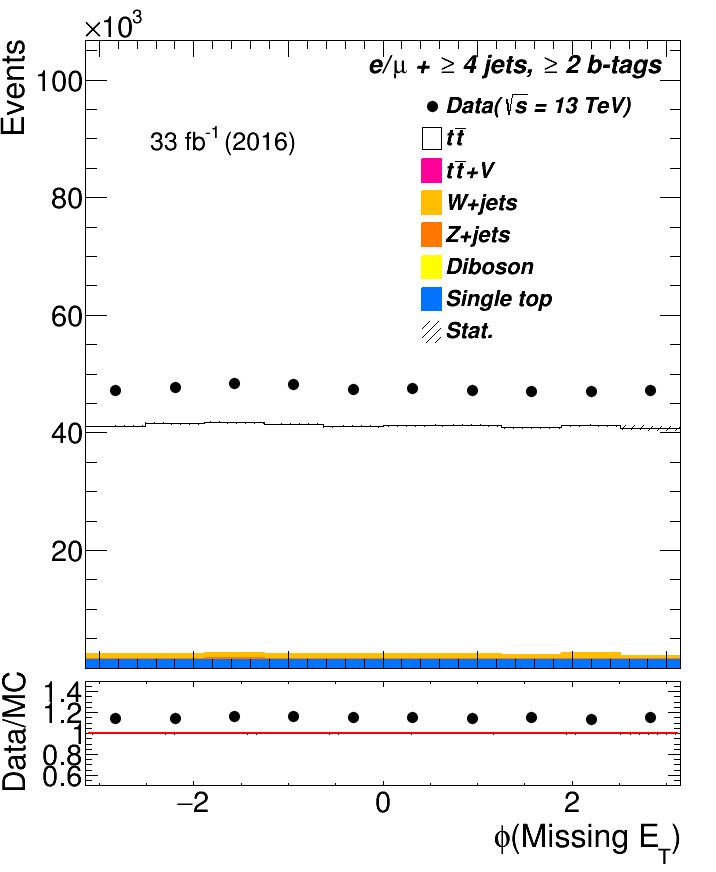
\includegraphics[width=\linewidth]{ControlPlots_emujets_2016_4incl_2incl/met_phi_emujets_2016.png}
	 	\caption{$\phi$ of $E_T^{miss}$.} \label{fig:Sec6}
	 \end{subfigure}

 
 

 \begin{subfigure}{0.25\textwidth}
 	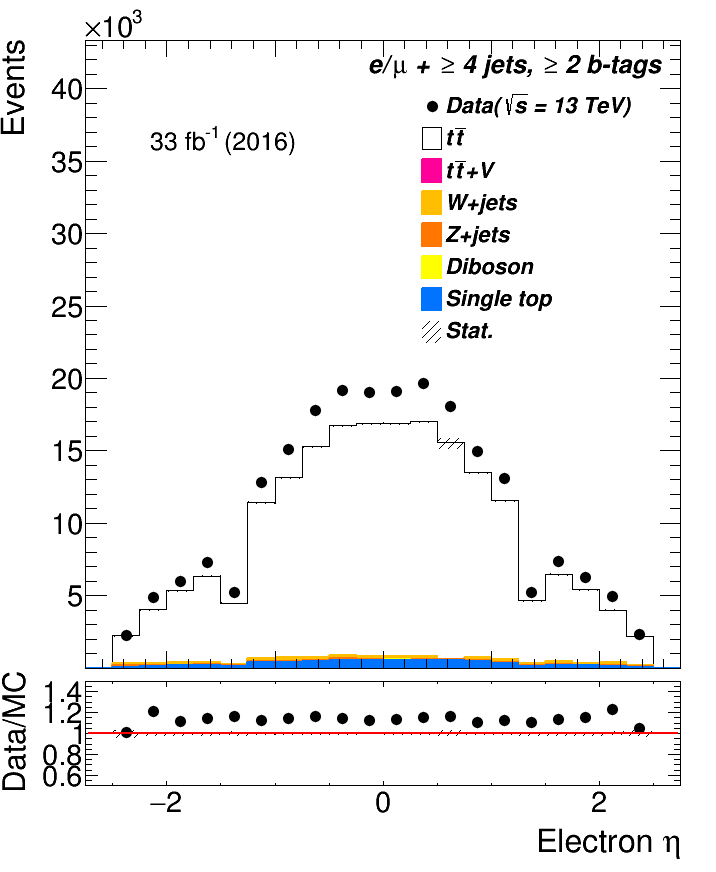
\includegraphics[width=\linewidth]{ControlPlots_emujets_2016_4incl_2incl/el_eta_emujets_2016.png}
 	\caption{$\eta$ of the electrons.} \label{fig:Sec9}
 \end{subfigure}\hspace*{0.5cm}
 \begin{subfigure}{0.25\textwidth}
 	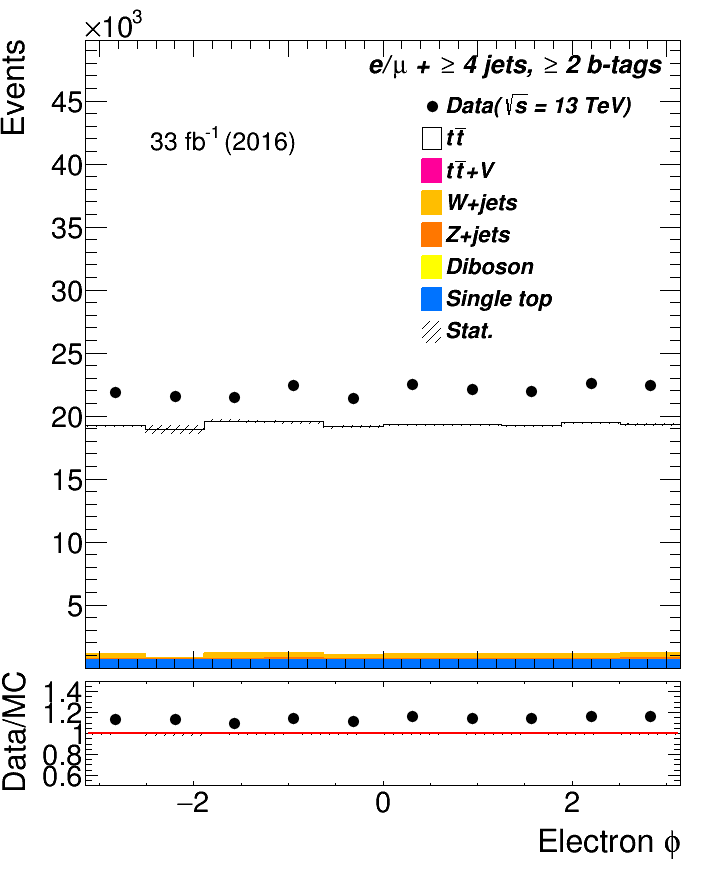
\includegraphics[width=\linewidth]{ControlPlots_emujets_2016_4incl_2incl/el_phi_emujets_2016.png}
 	\caption{$\phi$ of the electrons.} \label{fig:Sec10}
 \end{subfigure}\hspace*{0.5cm}
 \begin{subfigure}{0.25\textwidth}
 	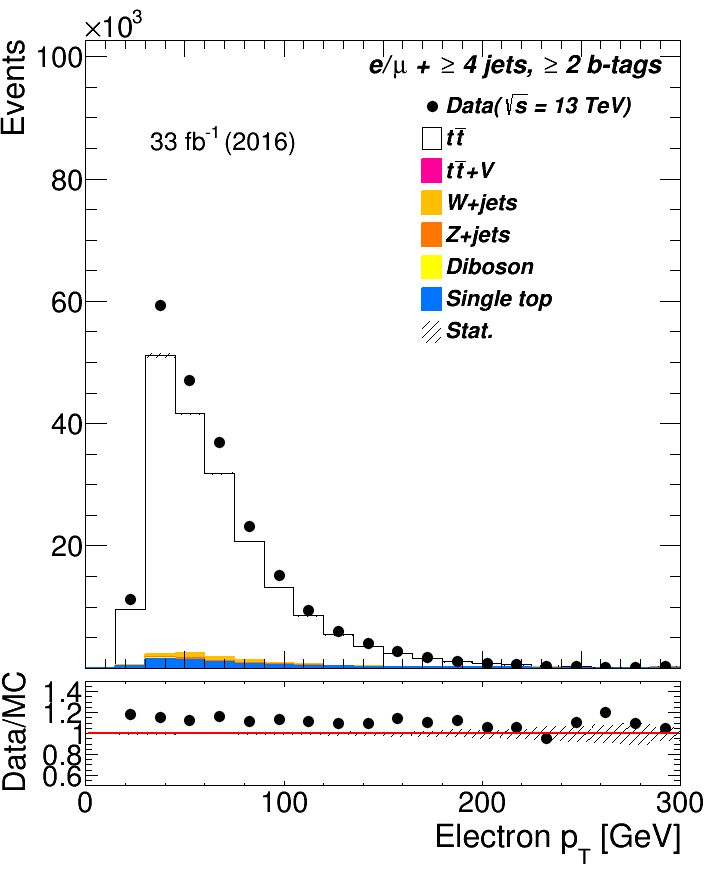
\includegraphics[width=\linewidth]{ControlPlots_emujets_2016_4incl_2incl/el_pt_emujets_2016.png}
 	\caption{Electron $p_T$.} \label{fig:Sec13}
 \end{subfigure}
 
 
 	
	\caption{Observed distributions after the event preselection. All events are observed in the lepton + jets decay channel and contain at least 4 jets and at least two $b$-tagged jets. The data is displayed by the black points. The solid histogram shows the signal-plus background predicted events, which are normalized to the number of events observed in data. The lower part shows the data-simulation agreement.}
	\label{fig:Sel1}
\end{figure}	


\begin{figure} % "[t!]" placement specifier just for this example
	\centering	


	\begin{subfigure}{0.25\textwidth}
	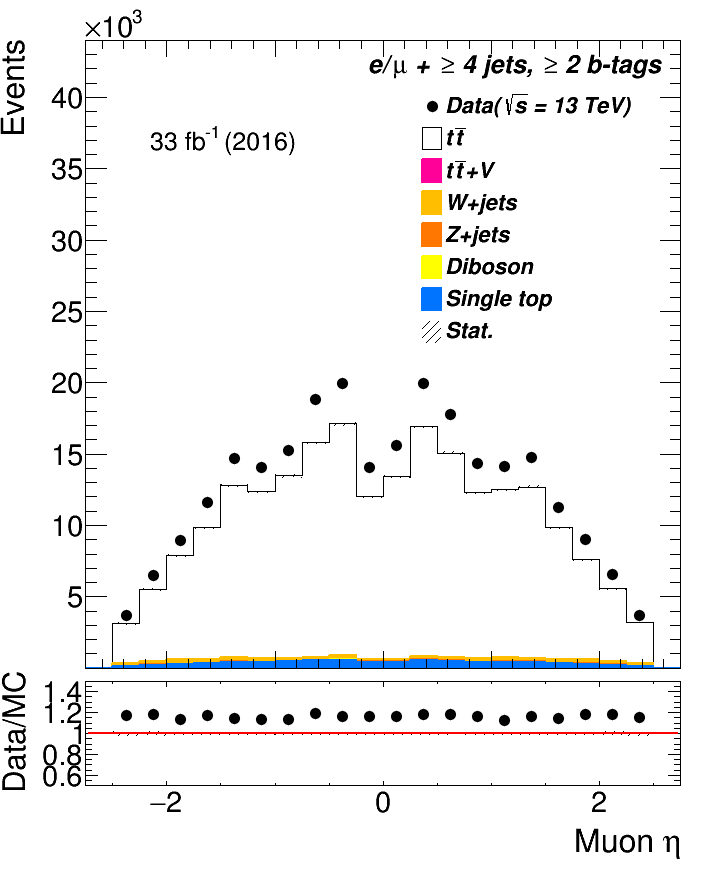
\includegraphics[width=\linewidth]{ControlPlots_emujets_2016_4incl_2incl/mu_eta_emujets_2016.png}
	\caption{$\eta$ the muons} \label{fig:Sec17}
\end{subfigure}\hspace*{0.5cm}
		\begin{subfigure}{0.25\textwidth}
	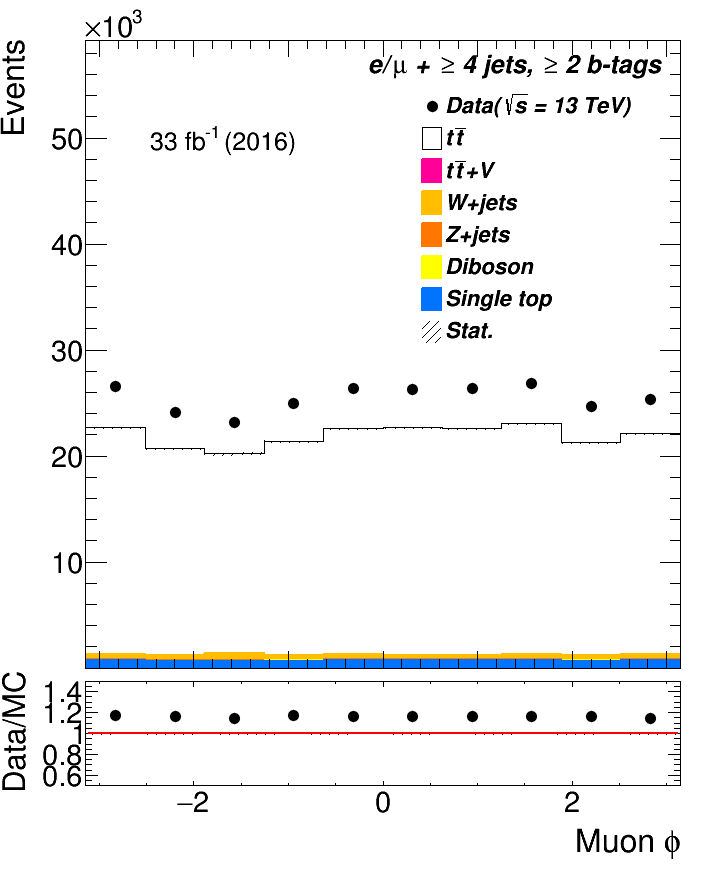
\includegraphics[width=\linewidth]{ControlPlots_emujets_2016_4incl_2incl/mu_phi_emujets_2016.png}
	\caption{$\phi$ of the muons.} \label{fig:Sec18}
\end{subfigure}\hspace*{0.5cm}
	\begin{subfigure}{0.25\textwidth}
		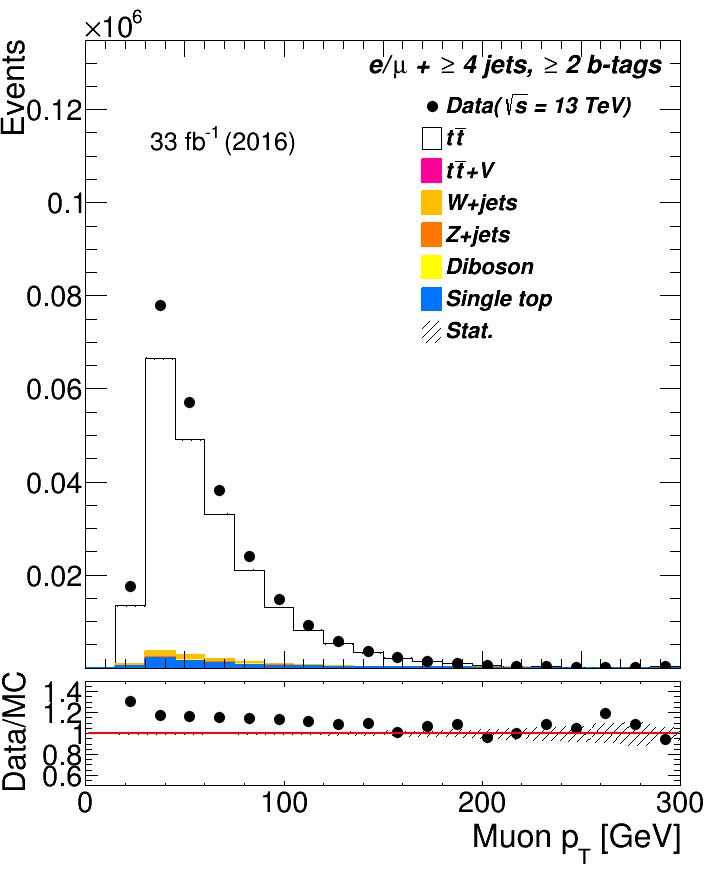
\includegraphics[width=\linewidth]{ControlPlots_emujets_2016_4incl_2incl/mu_pt_emujets_2016.png}
		\caption{Muon $p_T$.} \label{fig:Sec12}
	\end{subfigure}


	\begin{subfigure}{0.25\textwidth}
		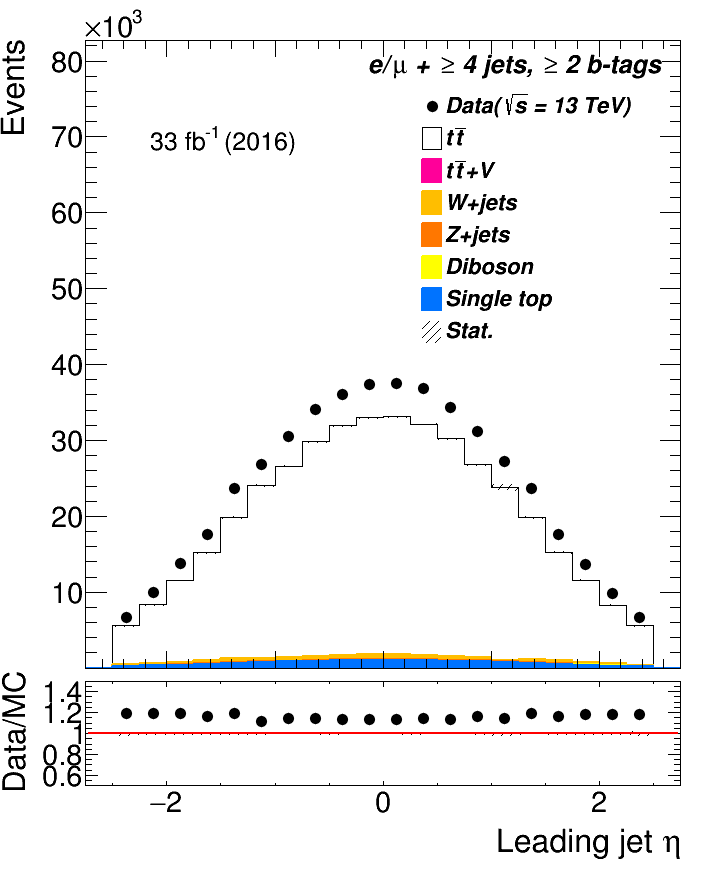
\includegraphics[width=\linewidth]{ControlPlots_emujets_2016_4incl_2incl/jet0_eta_emujets_2016.png}
		\caption{$\eta$ the first jet.} \label{fig:Sec19}
	\end{subfigure}\hspace*{0.5cm}
\begin{subfigure}{0.25\textwidth}
	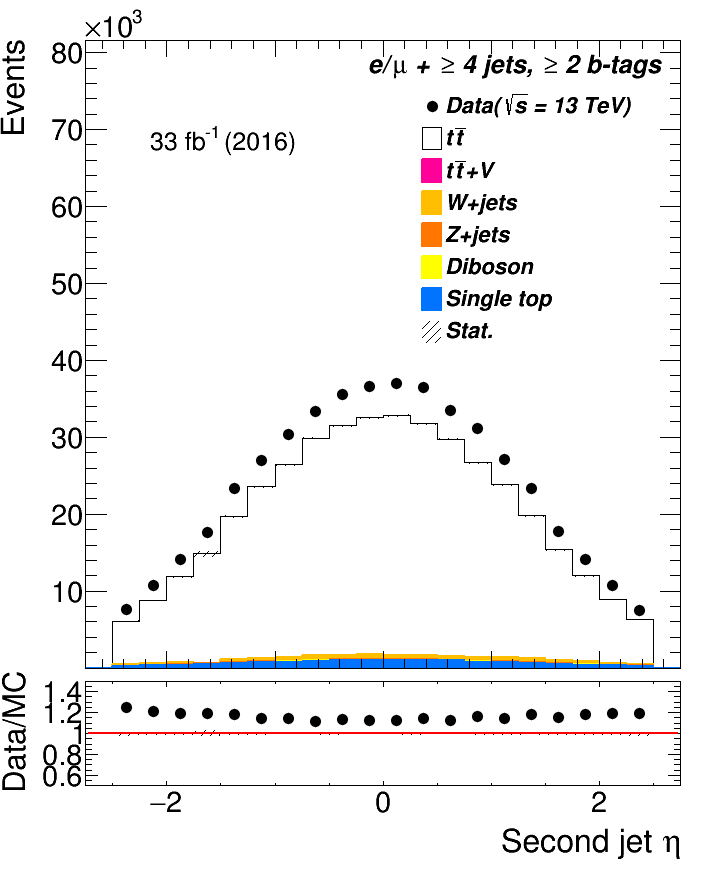
\includegraphics[width=\linewidth]{ControlPlots_emujets_2016_4incl_2incl/jet1_eta_emujets_2016.png}
	\caption{$\eta$ of the sec. jet.} \label{figSec23}
\end{subfigure}
\begin{subfigure}{0.25\textwidth}
	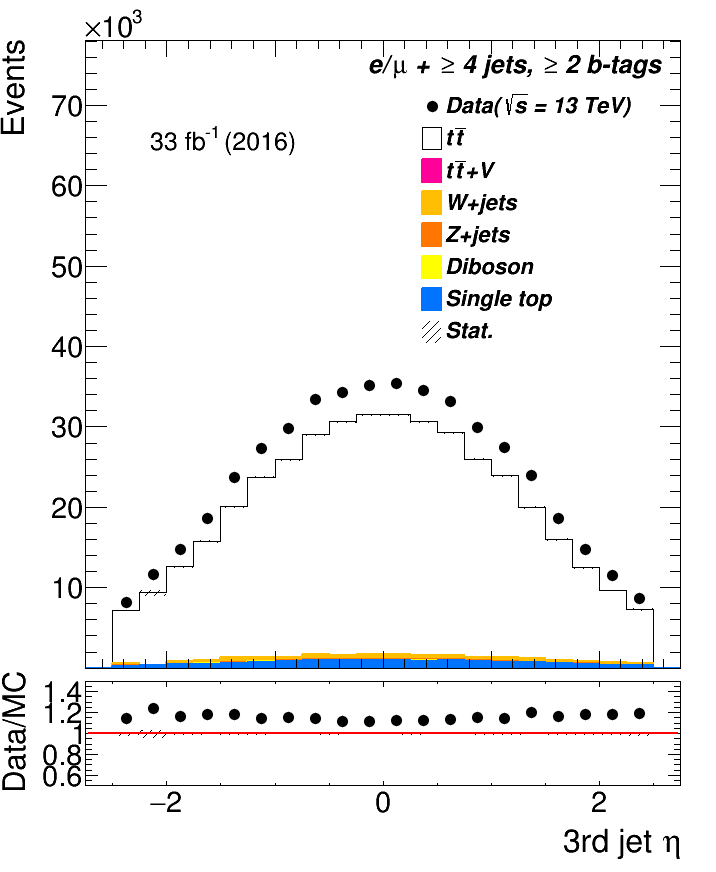
\includegraphics[width=\linewidth]{ControlPlots_emujets_2016_4incl_2incl/jet2_eta_emujets_2016.png}
	\caption{$\eta$ of the third jet.} \label{fig:Sec25}
\end{subfigure}

\begin{subfigure}{0.25\textwidth}
	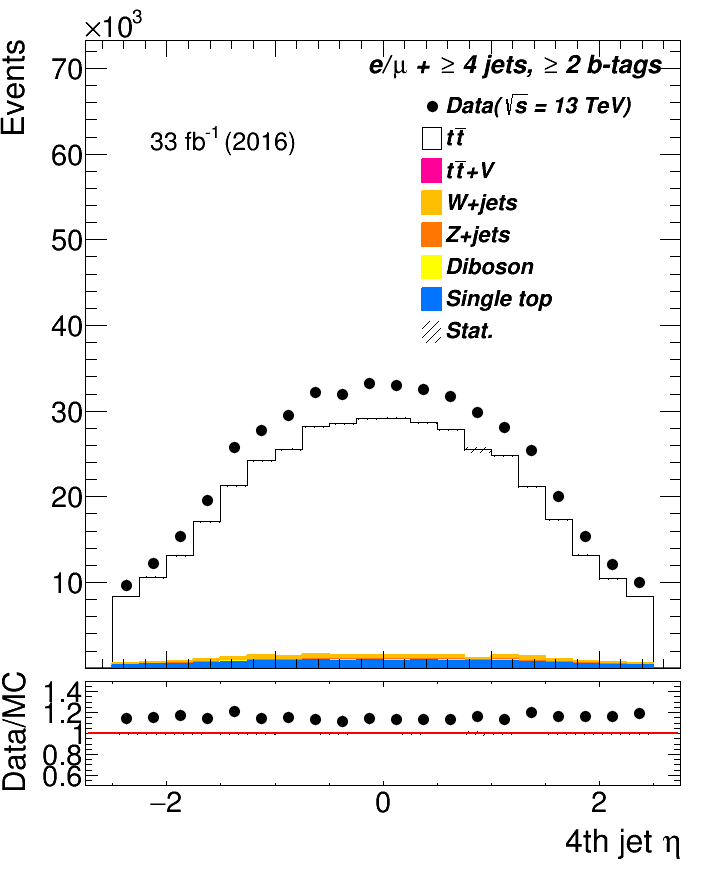
\includegraphics[width=\linewidth]{ControlPlots_emujets_2016_4incl_2incl/jet3_eta_emujets_2016.png}
	\caption{$\eta$ of the fourth jet.} \label{fig:Sec29}
\end{subfigure}



	
	\caption{As in~\cref{fig:Sel1}, global distributions are displayed for the muon, as well as for the four jets, obtained for the sample with at least 4 jets and at last two $b$-tagged jets.}	\label{fig:Sel2}
\end{figure}















\clearpage

\begin{figure} [t]% "[t!]" placement specifier just for this example
	\centering
	
	
	
	
	\begin{subfigure}{0.25\textwidth}
		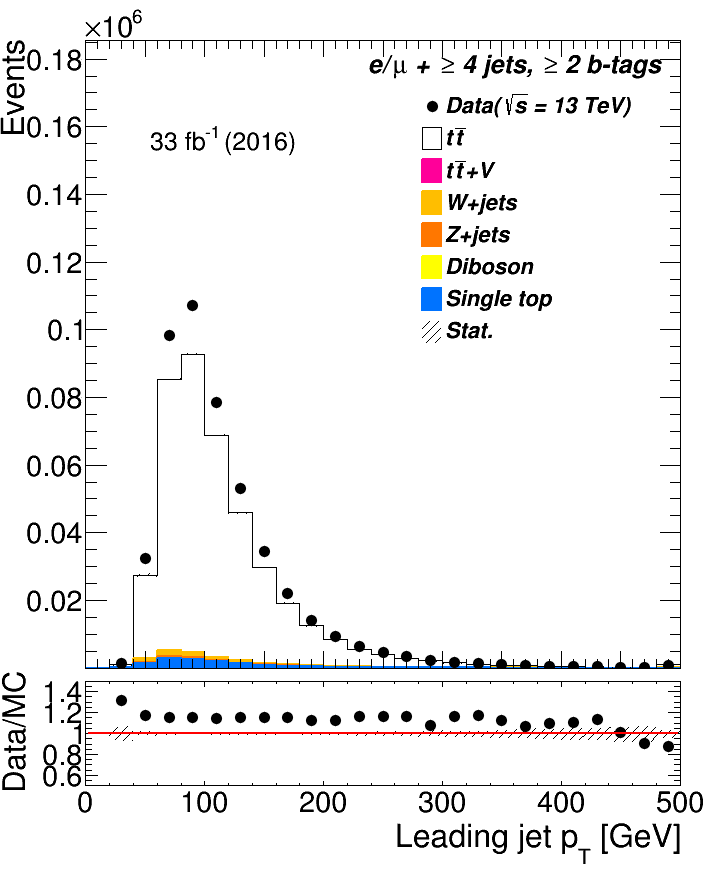
\includegraphics[width=\linewidth]{ControlPlots_emujets_2016_4incl_2incl/jet0_pt_emujets_2016.png}
		\caption{$p_T$ of the first jet.} \label{fig:Sec21}
	\end{subfigure}\hspace*{0.5cm}
	\begin{subfigure}{0.25\textwidth}
		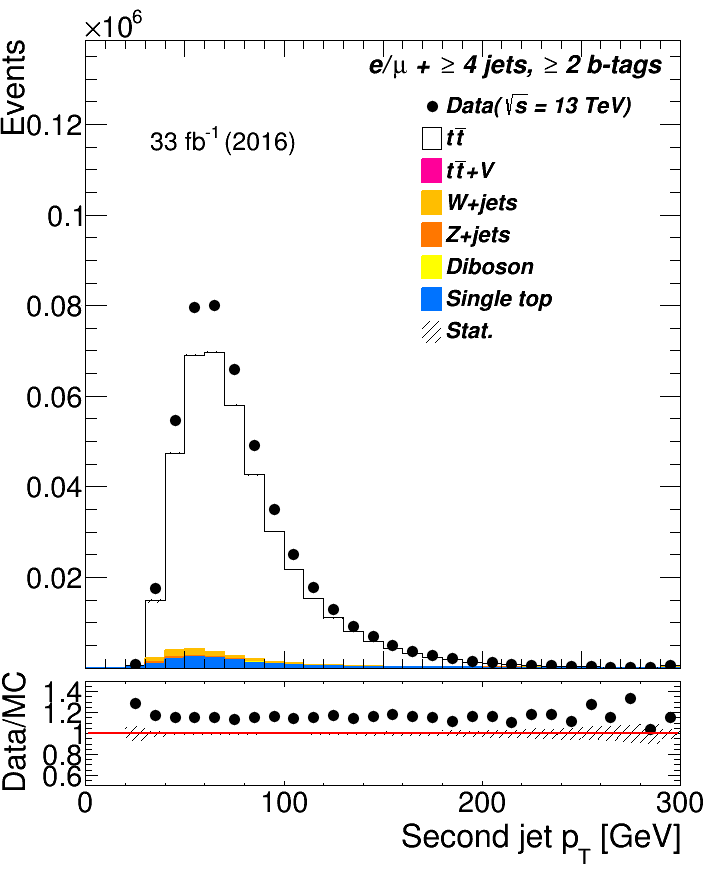
\includegraphics[width=\linewidth]{ControlPlots_emujets_2016_4incl_2incl/jet1_pt_emujets_2016.png}
		\caption{$p_T$ of the second jet.} \label{fig:Sec22}	
	\end{subfigure}
	
	
	
	\begin{subfigure}{0.25\textwidth}
		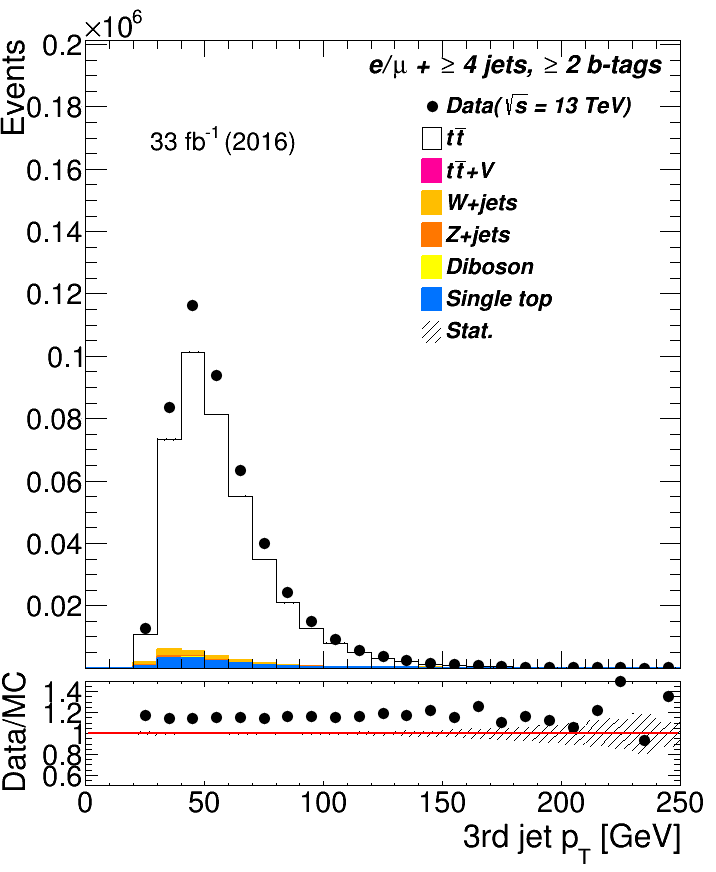
\includegraphics[width=\linewidth]{ControlPlots_emujets_2016_4incl_2incl/jet2_pt_emujets_2016.png}
		\caption{$p_T$ of the third jet.} \label{fig:Sec27}
	\end{subfigure}\hspace*{0.5cm}
	\begin{subfigure}{0.25\textwidth}
		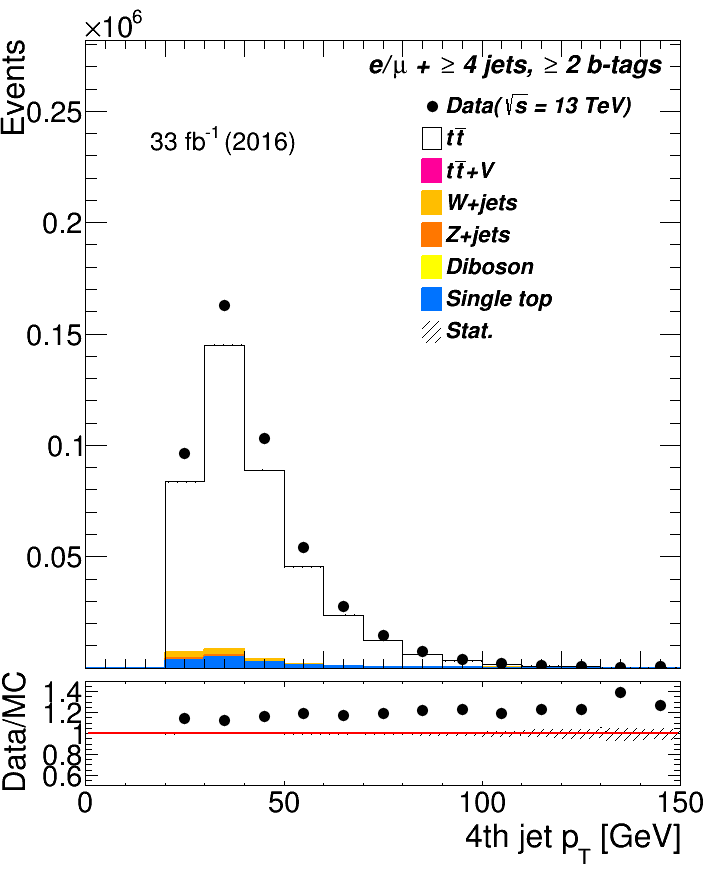
\includegraphics[width=\linewidth]{ControlPlots_emujets_2016_4incl_2incl/jet3_pt_emujets_2016.png}
		\caption{$p_T$ of the fourth jet.} \label{fig:Sec28}
	\end{subfigure}
	
	
	\caption{As in in~\cref{fig:Sel1}, transverse momentum distributions  for of the four jets, obtained for the sample with at least 4 jets and at last two $b$-tagged jets.}
	\label{fig:Sel4}
\end{figure}



\subsubsection{Global Reconstructed Quantities}


In the following the control distributions of the three observables that are used in this thesis are displayed in~\cref{fig:K3,fig:K4,fig:K5}, together with further  observables  reconstructed with \textsc{KLFitter}. 
All shown control distributions contain at least $4$-jets with at least two $b$-tagged jets.  In the ratio plots, the  corresponding data-simulation comparison is given. Only the statistical uncertainties are shown and the QCD-multijet background is not included. Further reconstructed distributions can be find in~\cref{sec:app0}. 



 Despite the general slight offset of the data points with  to the solid histogram lines of the simulation, the number of events for almost each simulated distribution, remains consistent with the observed numbers in data.

 For the hadronic top $p_T$ spectrum~\cref{fig:K10}, however, the distribution is softer in data than predicted by the simulation. This issue has also been discovered by the 8~TeV analysis, where it was studied extensively, with the result that it will only affect the measurement, if the observed deviations are not covered by the systematic uncertainties~\cite{ATLAS-CONF-2017-071}. Since this is not the case for the 8~TeV measurement, it is assumed that this observation will also not affect the analysis presented here. Further investigations are needed when all uncertainness are included in this analysis. 




 


\begin{figure} % "[t!]" placement specifier just for this example
	\centering




	\begin{subfigure}{0.25\textwidth}
		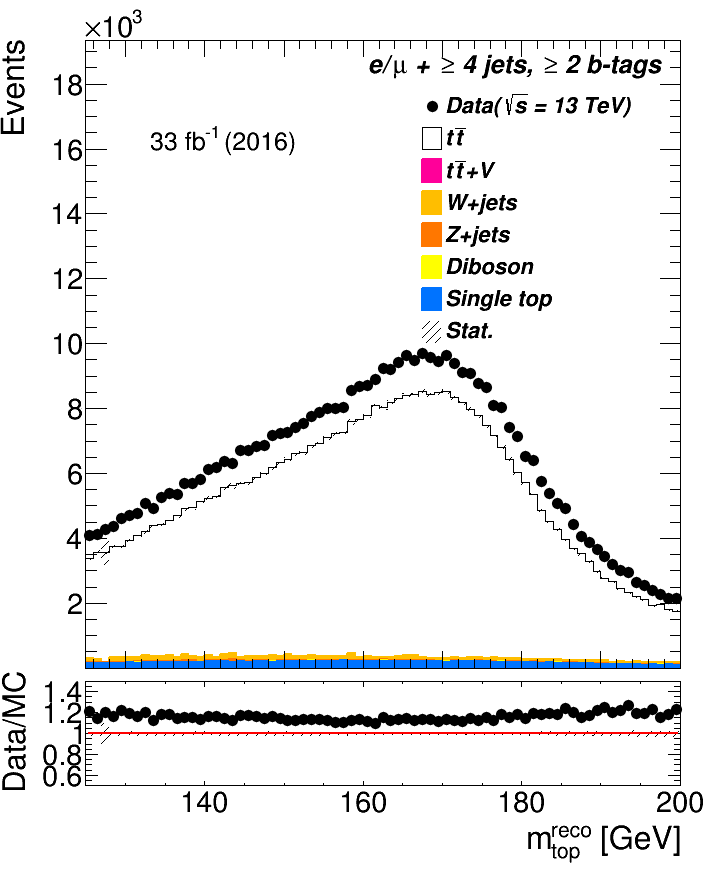
\includegraphics[width=\linewidth]{ControlPlots_emujets_2016_4incl_2incl//klf_window_mtop_reco_emujets_2016.png}
		\caption{Reconstructed hadronic top-quark mass $m_{\rm top}^{\rm reco}$.} \label{fig:K3}
	\end{subfigure}	\hspace*{0.5cm}
	\begin{subfigure}{0.25\textwidth}
		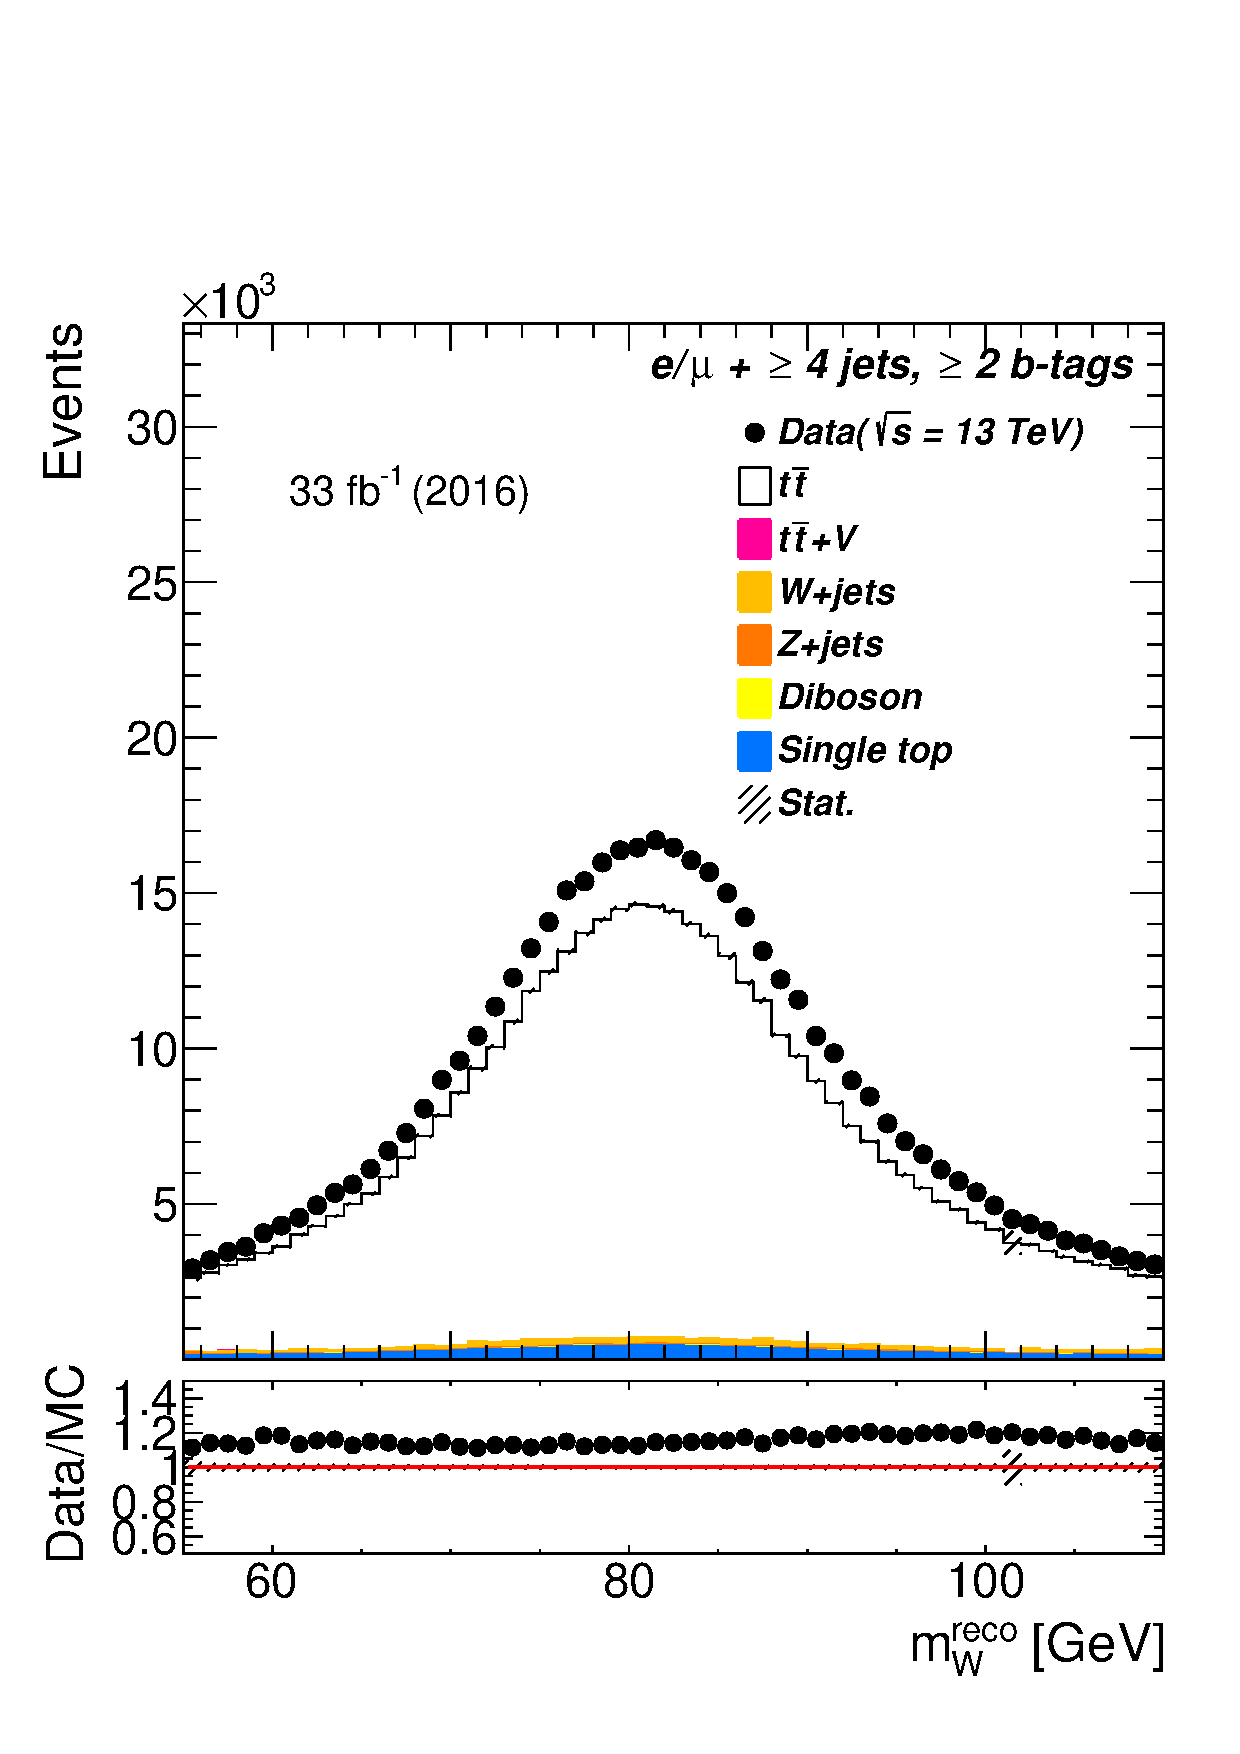
\includegraphics[width=\linewidth]{ControlPlots_emujets_2016_4incl_2incl/klf_window_mw_reco_emujets_2016.pdf}
		\caption{Reconstructed hadronic $W-boson$ mass $m_{\rm W}^{\rm reco}$.} \label{fig:K4}
	\end{subfigure}	\hspace*{0.5cm}	
	\begin{subfigure}{0.25\textwidth}
		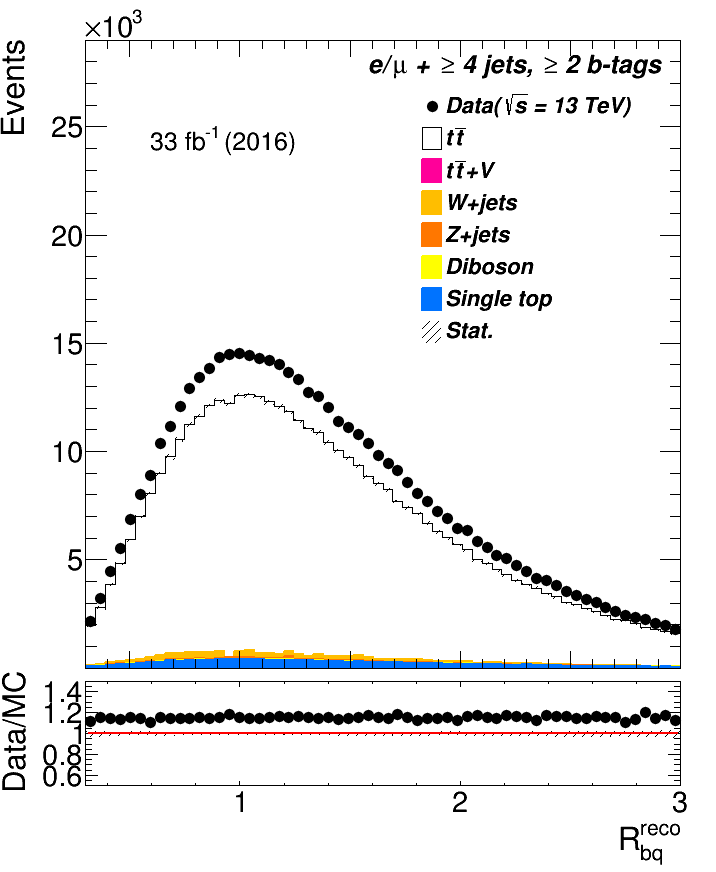
\includegraphics[width=\linewidth]{ControlPlots_emujets_2016_4incl_2incl/klf_window_rbq_reco_emujets_2016.png}
		\caption{Reconstructed $p_T$ ratio $R_{\rm bq}^{\rm reco}$.} \label{fig:K5}
	\end{subfigure}




\begin{subfigure}{0.25\textwidth}
	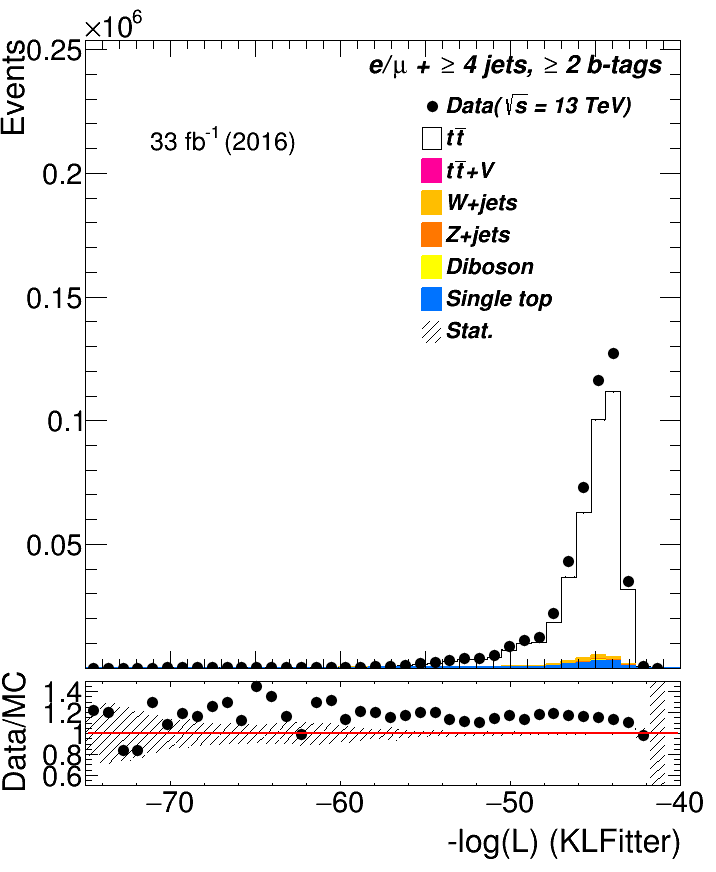
\includegraphics[width=\linewidth]{ControlPlots_emujets_2016_4incl_2incl/klf_LL_emujets_2016.png}
	\caption{The kinematic logarithmic \textsc{KLFitter} likelihood function.} \label{fig:K2}
\end{subfigure}\hspace*{0.5cm}	
	\begin{subfigure}{0.25\textwidth}
	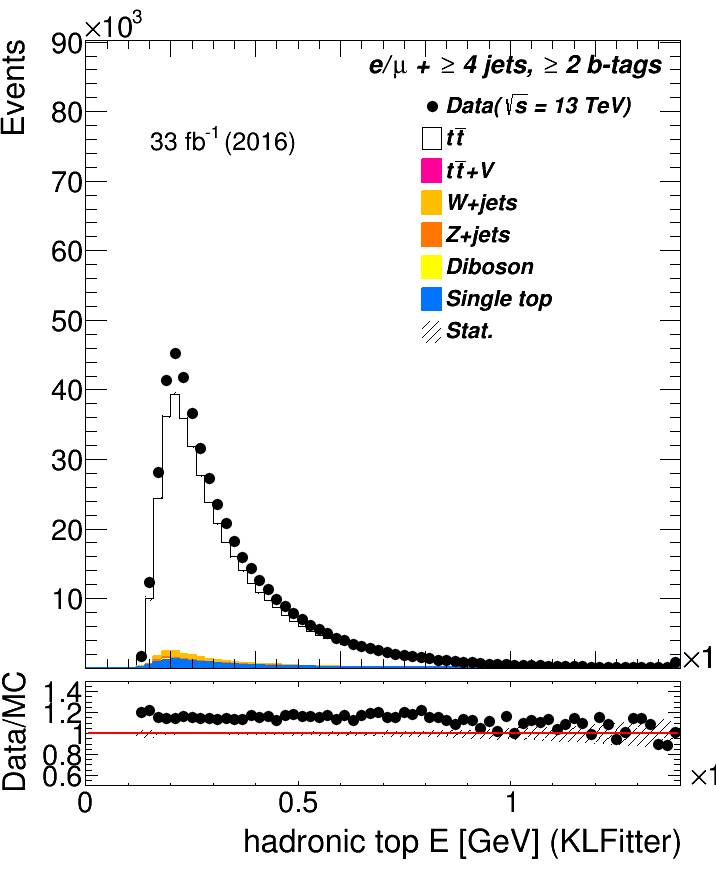
\includegraphics[width=\linewidth]{ControlPlots_emujets_2016_4incl_2incl/klf_topHad_E_emujets_2016.png}
	\caption{Energy of the hadronic top quark.} \label{fig:K7}
\end{subfigure}
\hspace*{0.5cm}
\begin{subfigure}{0.25\textwidth}
	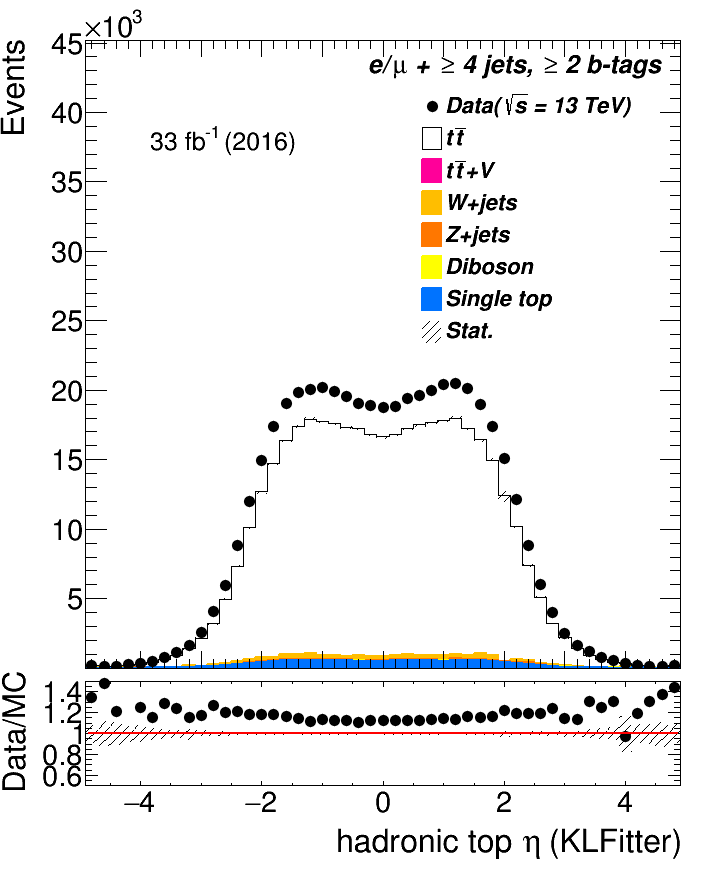
\includegraphics[width=\linewidth]{ControlPlots_emujets_2016_4incl_2incl/klf_topHad_eta_emujets_2016.png}
	\caption{$\eta$ of the hadronic top quark.} \label{fig:K8}
\end{subfigure}



	\begin{subfigure}{0.25\textwidth}
	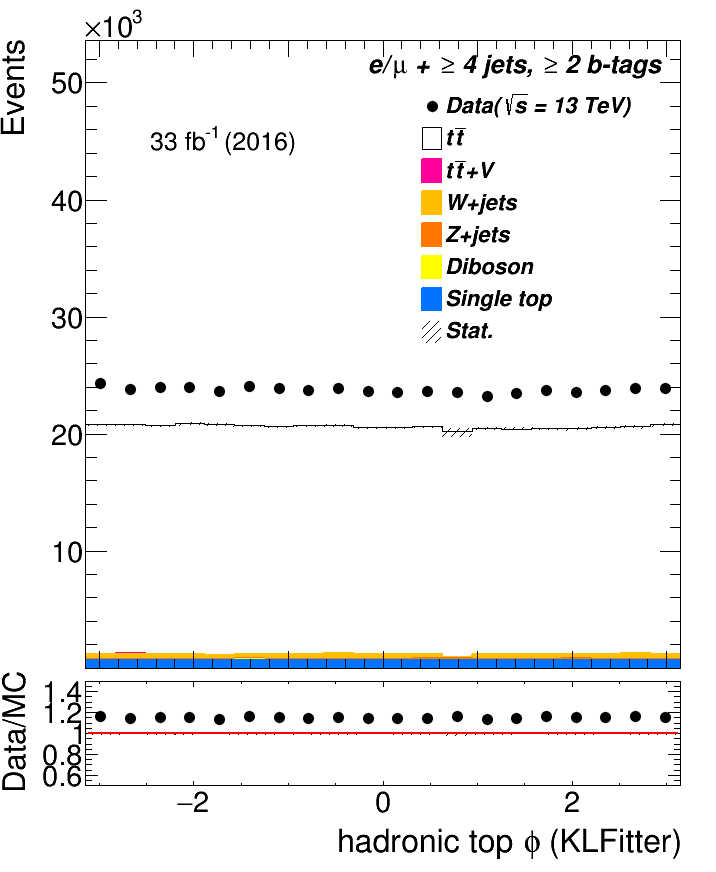
\includegraphics[width=\linewidth]{ControlPlots_emujets_2016_4incl_2incl/klf_topHad_phi_emujets_2016.png}
	\caption{$\phi$ of the hadronic top quark.} \label{fig:K9}
\end{subfigure}	
\hspace*{0.5cm}	
\begin{subfigure}{0.25\textwidth}
	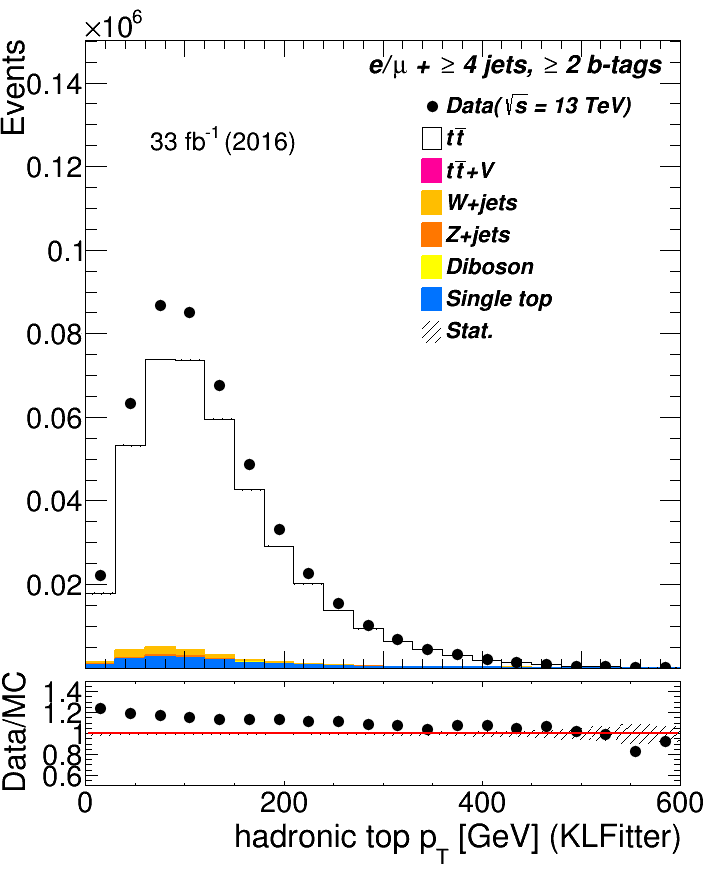
\includegraphics[width=\linewidth]{ControlPlots_emujets_2016_4incl_2incl/klf_topHad_pt_emujets_2016.png}
	\caption{Transverse momentum of the hadronic top quark.} \label{fig:K10}
\end{subfigure}\hspace*{0.5cm}
\begin{subfigure}{0.25\textwidth}
	\includegraphics[width=\linewidth]{ControlPlots_emujets_2016_4incl_2incl/klf_topLEP_E_emujets_2016.png}
	\caption{Energy of the leptonic top quark.} \label{fig:K11}
\end{subfigure}

\caption{Reconstructed global quantities, obtained with \textsc{KLFitter}. The black points represent the data, while the simulation is denoted by the solid histogram. The simulation of the different background processes are also shown by the coloured histograms. The data-simulation agreement is shown by the lower plot. Only statical errors are considered and the QCD-multijet background  is missing. The log-likelihood distribution is used by \textsc{KLFitter}, to obtain the best jet-patron assignment. The hadronic top-quark and  $W$-boson mass, as well as $R_{\rm bq}^{\rm reco}$ are very important quantities, which are generated from the event kinematics. If not mentioned different, the term hadronic or leptoinc, refer to the corresponding decay of the top-quark pair.}\label{klf100}
\end{figure}	



\begin{figure} % "[t!]" placement specifier just for this example
	\centering

	\begin{subfigure}{0.25\textwidth}
		\includegraphics[width=\linewidth]{ControlPlots_emujets_2016_4incl_2incl/klf_topLep_eta_emujets_2016.png}
		\caption{$\eta$ of the leptonic top quark.} \label{fig:K12}
	\end{subfigure}	\hspace*{0.5cm}
	\begin{subfigure}{0.25\textwidth}
	\includegraphics[width=\linewidth]{ControlPlots_emujets_2016_4incl_2incl/klf_topLep_phi_emujets_2016.png}
	\caption{$\phi$ of the leptonic top quark.} \label{fig:K13}
\end{subfigure}
\hspace*{0.5cm}
\begin{subfigure}{0.25\textwidth}
	\includegraphics[width=\linewidth]{ControlPlots_emujets_2016_4incl_2incl/klf_topLep_eta_emujets_2016.png}
	\caption{$\eta$ of the leptonic top-quark.} \label{fig:K14}
\end{subfigure}



	
	
	\begin{subfigure}{0.25\textwidth}
		\includegraphics[width=\linewidth]{ControlPlots_emujets_2016_4incl_2incl/klf_topLep_pt_emujets_2016.png}
		\caption{Transverse momentum of the leptonic quark.} \label{fig:K15}
	\end{subfigure}	\hspace*{0.5cm}
	\begin{subfigure}{0.25\textwidth}
		\includegraphics[width=\linewidth]{ControlPlots_emujets_2016_4incl_2incl/klf_topLep_m_emujets_2016.png}
		\caption{ Invariant mass of the leptonic top quark.} \label{fig:K16}
	\end{subfigure}\hspace*{0.25cm}
	\begin{subfigure}{0.25\textwidth}
		\includegraphics[width=\linewidth]{ControlPlots_emujets_2016_4incl_2incl/klf_ttbar_E_emujets_2016.png}
		\caption{Energy of the top-quark pair.} \label{fig:K17}
	\end{subfigure}


	\begin{subfigure}{0.25\textwidth}
		\includegraphics[width=\linewidth]{ControlPlots_emujets_2016_4incl_2incl/klf_ttbar_eta_emujets_2016.png}
		\caption{Rapidity of the top-quark pair.} \label{fig:K18}
	\end{subfigure}
	\hspace*{0.5cm}
	\begin{subfigure}{0.25\textwidth}
		\includegraphics[width=\linewidth]{ControlPlots_emujets_2016_4incl_2incl/klf_ttbar_phi_emujets_2016.png}
		\caption{$\phi$  distribution of the top-quark pair.                       } \label{fig:K19}
	\end{subfigure}
\hspace*{0.5cm}
	\begin{subfigure}{0.25\textwidth}
		\includegraphics[width=\linewidth]{ControlPlots_emujets_2016_4incl_2incl/klf_ttbar_pt_emujets_2016.png}
		\caption{Transverse momentum of the top-quark pair.} \label{fig:K20}
	\end{subfigure}
	
	\caption{Same plots as for~\cref{klf100} of the  global properties of the leptonic and hadronic top-quark, as well as of the top-quark pair, reconstructed with \textsc{KLFitter}.  }
\end{figure}	














%------------------------------------------------------------------------------
\chapter{Measurement of top-quark mass}
\label{sec:Temp1}
%------------------------------------------------------------------------------

The event selection and \rm reconstruction are the base for the final analysis step, which is required to determine the mass of the top-quark. In this final step, the template method  is adopted to determine $m_{\text{top}}$  from Monte Carlo (MC) simulated distributions of observables, which are sensitive to the mass value. These MC simulated samples are generated for different input values of $m_{\text{top}}$ and parametrized with analytical functions, which represent probability densities. These probabilities are used to determine the top-quark mass in an unbinned maximum likelihood fit.

 The template method is a standard analysis tool in high energy physics. However, there are certain issues affecting the measurement of the top-quark mass.  Hence, a unique approach has been developed and applied very successfully for the 7 and 8~TeV measurements~\cite{Aad:2015nba,ATLAS-CONF-2017-071}.

In the following the complete template parametrization is discussed in detail. Furthermore, the likelihood fit and the necessary analysis related assumptions are explained. Finally, the consistency of the fit procedure is tested. 


\section{3D-template method}
The measurement of the top-quark mass with the template method, suffers from large uncertainties, which arise from the jet energy scale (JES) and the $b$-to-light jet energy scale (bJES), which is related to energy calibration of $b$-jets. The large impact of the JES uncertainties on the top mass measurement has been shown by previous top-quark mass measurements. For  the 7~TeV analysis, the JES uncertainty is with 0.58 $ \pm $ 0.11~GeV ~\cite{Aad:2015nba} one of the largest systematics, as well as for  the 8~TeV measurement, where the JES uncertainty is 0.54 $\pm$ 0.11~GeV~\cite{ATLAS-CONF-2017-071}.

 The basic idea to face the large jet energy scale uncertainties, is to measure the top-quark mass simultaneously with the jet energy scale factor (JSF) and the $b$-to-light jet energy scale factor (bJSF). The et energy scale factors are introduced to provide the necessary sensitivity to the jet energy scales. The simultaneous determination of these three variables allows to absorb the effects arising from energy scale variations, by making use of the multidimensionality of the fit. 
However, in order to make use of the higher dimensionality of the fit, one needs enough statics to consider the sum in quadrature of the systematic uncertainties as small, compared to JES and bJES uncertainties~\cite{ATLAS-CONF-2017-071}. 



The success of the three dimensional approach can be seen by the remarkable results from the 8~TeV measurement. There, the template fit is performed for one, two and three dimensions, which demonstrates the  effect of the higher dimensional fit on the corresponding uncertainties. The achieved improvement of a two dimensional fit, i.e. the determination of $m_{\text{top}}$ and JSF, compared to a one dimensional fit where only $m_{\text{top}}$ is measured, is  8.3~\% of the final error on $m_{\text{top}$~\cite{ATLAS-CONF-2017-071}.
Moreover, the additional measurement of  bJSF improves the total uncertainty about 43~\%~\cite{ATLAS-CONF-2017-071}.
 Despite these impressive results, one has to keep in mind that the situation might be different for the 13~TeV analysis and a qualified statement can only be given after the first evaluation of all uncertainties.

 The three observables used in the analysis here have already been introduced in~\cref{ch5}.
The first estimator is the \rm reconstructed top-quark mass $m_{\text{top}}^{\rm reco}$, which is obtained from the kinematic likelihood fit of the event \rm reconstruction.
From the corresponding  jet permutation of the \textsc{KLFitter} output, the \rm reconstructed $W$-boson mass $m_{\text{W}}^{\rm reco}$ is used, as well as the third variable $R_{\text{bq}}^{\rm reco}$. While $m_{\text{top}}^{\rm reco} $ is determined as free parameter of the kinematic likelihood fit,  the other two are built from the original four vectors.  $R_{\text{bq}}^{\rm reco}$ is here calculated with the two $b$-tag definition. For all three of these \rm reconstructed estimators, Monte Carlo simulated distributions are generated, with an input top-quark mass value between 170.0 and 175.0~GeV. The nominal sample has a mass of 172.5~GeV. Furthermore, all of these distributions are calculated for different scale factors. 
If the JSF is varied (between 0.96 and 1.04) the bJSF is set to unity and vice versa.
 In~\cref{fig:Comparison} the sensitivities of the estimator distributions to different values for $m_{\text{top}}$, JSF and bJSF are shown and compared to 
the nominal sample (red). For each sample, only one variable is varied, while the rest are set to the nominal values, which is 172.5~GeV for $ m_{\text{top}}$ and 1.00 for both scale factors. The deviations from the nominal samples are displayed in the ratio plot below. 
As it can be seen in~\cref{fig:mtopmtop,fig:mtopJSF,fig:mtopbJSF}, the first estimator  $m_{\text{top}}^{\rm reco}$  shows a noticeable sensitivity to all three variables, while $m_{\text{W}}^{\rm reco}$ only varies with the jet energy scale factor (JSF) (see~\cref{fig:mwmtop,fig:mwJSF,fig:mwbJSF}).  The third observable $R_{\text{bq}}^{\rm reco}$ (~\cref{fig:Rbqmtop,fig:RbqJSF,fig:RbqbJSF}), shows a weak sensitivity to the JSF variations, compared to its dependency on the $b$-to-light jet energy scale factor (bJSF). The scale factors are  multiplicative quantities and reduce or increase the number of events  passing the event selection cuts. Events with a higher scale factor, compared to the nominal one, are more likely to pass the event selection than those of samples with a lower scale factor.

 The displayed distributions in~\cref{fig:Comparison} are already normalized to one and parametrized with analytical functions, which are basically the sum of  Gaussians and Landau distributions. From the parametrized templates, the probability density functions for the unbinned maximum likelihood fit are constructed. 
 
 

The parametrization of the templates is one of the major tasks of this thesis. This part has been implemented completely new, based on the method of the previous measurements. 

In the following the different steps of the template parametrization are introduced together with corresponding results. If not mentioned otherwise, all shown distributions are normalized to one. 



\begin{landscape}
	

\begin{figure} % "[t!]" placement specifier just for this example
	\centering 
	

	\begin{subfigure}{0.37\textwidth}
		\includegraphics[width=\linewidth]{Pics/PlotCombi/mtop_mtop.png}
		\caption{$m_{top}^{reco}$ vs $m_{top}$} \label{fig:mtopmtop}
	\end{subfigure}
	\hspace*{0.25cm}
	\begin{subfigure}{0.37\textwidth}
	\includegraphics[width=\linewidth]{Pics/PlotCombi/mtop_JSF.png}
	\caption{$m_{top}^{reco}$ vs JSF} \label{fig:mtopJSF}
	\end{subfigure}
	\hspace*{0.25cm}
	\begin{subfigure}{0.37\textwidth}
	\includegraphics[width=\linewidth]{Pics/PlotCombi/mtop_bJSF.png}
	\caption{$m_{top}^{reco}$ vs bJSF} \label{fig:mtopbJSF}
	\end{subfigure}
	\begin{subfigure}{0.37\textwidth}
	\includegraphics[width=\linewidth]{Pics/PlotCombi/mw_mtop.png}
	\caption{$m_{W}^{reco}$ vs $m_{top}$} \label{fig:mwmtop}
	\end{subfigure}
	\hspace*{0.25cm}
	\begin{subfigure}{0.37\textwidth}
	\includegraphics[width=\linewidth]{Pics/PlotCombi/mw_JSF.png}
	\caption{$m_{W}^{reco}$ vs JSF} \label{fig:mwJSF}
	\end{subfigure}
	\hspace*{0.25cm}
	\begin{subfigure}{0.37\textwidth}
	\includegraphics[width=\linewidth]{Pics/PlotCombi/mw_bJSF.png}
	\caption{$m_{W}^{reco}$ vs bJSF} \label{fig:mwbJSF}
	\end{subfigure}
	\begin{subfigure}{0.37\textwidth}
	\includegraphics[width=\linewidth]{Pics/PlotCombi/rbq_mtop.png}
	\caption{$R_{bq}^{reco}$ vs $m_{top}$} \label{fig:Rbqmtop}
\end{subfigure}
\hspace*{0.25cm}
\begin{subfigure}{0.37\textwidth}
	\includegraphics[width=\linewidth]{Pics/PlotCombi/rbq_JSF.png}
	\caption{$R_{bq}^{reco}$ vs JSF} \label{fig:RbqJSF}
\end{subfigure}
\hspace*{0.25cm}
\begin{subfigure}{0.37\textwidth}
	\includegraphics[width=\linewidth]{Pics/PlotCombi/rbq_bJSF.png}
	\caption{$R_{bq}^{reco}$ vs bJSF} \label{fig:RbqbJSF}
\end{subfigure}
	\caption{Comparison of signal $t\bar{t}$ templates for different simulated top-quark masses and scale factors. For each of the three observables, ($m_{top}^{reco}$, $m_{W}^{reco}$ and $R_{bq}^{reco}$) the sensitivities are displayed, by overlaying the nominal (red) sample with samples for different JSF, bJSF and $m_{top}$ . The unvaried quantity is kept to the nominal value. }
\end{figure}\label{fig:Comparison}	
\end{landscape}
  
  
\clearpage  

\subsubsection{The template parametrization}


The parametrization of the estimator distributions, consists of several sub-steps. Firstly, the actual parametrization, which is used to obtain the probability densities, is performed. The procedure is briefly as follows: 
\begin{itemize}
	\item First of all, each single distribution is fitted with the analytical functions described below to obtain a set of parameters ($p_i$ with $i$ =0,1,...).
	\item The fitted parameters are parametrized linear as functions of $m_{\text{top}}$, JSF and bJSF. 
	\item With parameters from the two steps above, as initial values, a combined fit is performed to obtain the final parametrization of the templates.
\end{itemize}   

 
 In case of this thesis,  only templates of signal events are used to perform a first test of the method. However, the major changes, which have to be considered for the inclusion of the background samples are also taken into account in following.  


\subsubsection{The single fits}  


 At the beginning of the parametrization process, the best possible initial conditions are searched for the  combined fit of the templates. Furthermore, one is also interested in the dependencies between the three estimators ($m_{\text{top}}^{\rm reco}$, $m_{\text{W}}^{\rm reco}$ and $R_{\text{bq}}^{\rm reco}$) and the three observables, which are of interest ($m_{\text{top}}$, JSF and bJSF). Therefore, two interpolation steps are performed. 

 First of all, each single \rm reconstructed template is fitted with a  analytical function. For  $m_{\text{top}}^{\rm reco}$  and  $m_{\text{W}}^{\rm reco}$, this is the sum of a Gaussian, a normal Landau function and a mirrored Landau function.  $R_{\text{bq}}^{\rm reco}$ is fitted with the sum of two gaussians and one Landau distribution. 
Since $m_{W}^{\rm reco}$ does not show any significant sensitivities on $m_{\text{top}}$ and bJSF, only the samples with different JSF are parametrized. 
In the analysis published in~\cite{ATLAS-CONF-2017-071}, the $m_{\text{W}}^{\rm reco}$ distribution was parametrized  by the sum of two Gaussians. In this thesis however it has been found that the sum of a Gaussian, a Landau and a mirrored Landau distribution describes the observable better.
 
 From the fist parametrization steps nine parameters ($p_i$) are obtained for each fitted sample of all three distributions ($m_{\text{top}}^{\rm reco}$, $m_{\text{W}}^{\rm reco}$ and $R_{\text{bq}}^{\rm reco}$). The  parameters  represent the amplitude, the mean and the standard deviation of the fit functions. The detailed assignment of the functions can be find in~\cref{tab:parameters}. All parameters of the different sets with same index $i$  are plotted against the simulated $m_{\rm top}$, JSF and bJSF of the corresponding sample. The plots are parametrized with linear functions.  Each parameter ($p_i$) can than be written in the following form:
\begin{eqnarray}
&&p_i = a_{\rm 0i} + a_{\rm 1i} m_{\text{top}}, \nonumber \\
&& p_i = b_{\rm 0i} + b_{\rm 1i}(\text{JSF} - 1.00) \hspace{0.5cm}     \text{and}      \nonumber \\   
&& p_i = c_{\rm 0i} + c_{\rm 1i}(\text{bJSF - 1.00}). \nonumber    \\
\end{eqnarray}
The parameters are described by the slope and the offset of the linear functions. All parameters which are determined in these two steps  are used  as initial parameters  for the combined template parametrization.
\clearpage
\begin{center}
	\captionof{table}{Assingment of the fit paramertes and the analytical functions. $A$ denotes the amplitude of the function, $\mu$ the mean and $\sigma$ the standard deviation.}\label{tab:parameters}
	
	
	
	\vspace{0.3cm}	
	\begin{tabular}{>{}m{3.0cm}>{}m{3.0cm} >{}m{3.0cm}>{}m{3.0cm} } \toprule
		
		Parameter&   $m_{\text{top}^{reco}}$&  $m_{\text{W}^{reco}}$ & $R_{\text{bq}^{reco}}$\\
		\midrule
		$p_0$ & $A$ Gaussian& $A$ Gaussian &$A$ Gaussian 1\\
		$p_1$ &  $\mu$ Gaussian& $\mu$ Gaussian & $\mu$ Gaussian 1\\
		$p_2$ &  $\sigma$ Gaussian& $\sigma$ Gaussian&$\sigma$ Gaussian1\\
		$p_3$ & $A$ Landau            & $A$ mirrored Landau &$A$ Gaussian 2\\
		$p_4$ &  $\mu$ Landau      & $\mu$ mirrored Landau& $\mu$ Gaussian 2\\
		$p_5$ &  $\sigma$ Landau   & $\sigma$ mirrored Landau&$\sigma$ Gaussian 2 \\
		$p_6$ & $A$ mirrored Landau & $A$  Landau}&$A$ Landau\\
	$p_7$ &  $\mu$ mirrored Landau& $\mu$ Landau& $\mu$ Landau\\
	$p_8$ &  $\sigma$ mirrored Landau& $\sigma$ Landau&$\sigma$ Landau\\
	
	\bottomrule
		\vspace{1.0cm}	
\end{tabular}

\end{center}

\begin{figure} % "[t!]" placement specifier just for this example
	\centering 
	
	
	\begin{subfigure}{0.45\textwidth}
		\includegraphics[width=\linewidth]{Pics/Linear/{Lin0_d0_p2_n}.png}
		\caption{$m_{\text{top}}^{\rm reco}$ P2 vs $m_{\text{top}}$} \label{fig:lin1}
	\end{subfigure}
	\hspace*{0.2cm}
	\begin{subfigure}{0.45\textwidth}
		\includegraphics[width=\linewidth]{Pics/Linear/{Lin0_d1_p1_n}.png}
		\caption{$m_{\text{W}}^{\rm reco}$ P1 vs JSF} \label{fig:lin2}
	\end{subfigure}

	\begin{subfigure}{0.45\textwidth}
	\includegraphics[width=\linewidth]{Pics/Linear/{Lin0_d2_p3_n}.png}
	\caption{$R_{\text{bq}}^{\rm reco}$ P3 vs bJSF} \label{fig:lin3}
\end{subfigure}
	\caption{Linear parametrization $p_i$ of the parameters, obtained by the single template fits. Selected parameters are fitted against the different simulated values of $m_{\text{top}}$ and the scale factors. For the scale factors, only the differences from the nominal value $\Delta$, are displayed.}\label{fig:linear1}
\end{figure}



 In~\cref{fig:linear1} examples of the linear parametrization of the fitted parameters, which belong to the single template fit, are shown. The parameters of the different individual $m_{\text{top}}^{\rm reco}$ template fits are plotted against the simulated top-quark mass, and the different JSF and bJSF.  In analogy, there are linear parametrizations of the same kind for  $R_{\text{bq}}^{\rm reco}$, while for $m_{\text{W}}^{\rm reco}$ there is only a linear fit in terms of the jet energy scale JES. The linear dependencies between the parameters of the estimator fits and the observables are essential for the analysis. This will become more clear below with the introduction of the simultaneous parametrization. Only if the distributions are well described and the linearity of each parameter has been achieved, the results of the single fits can be used to perform the simultaneous fit to the estimator distribution. 

 The complete linear fit of all  parameters and the corresponding plots can be find in~\cref{sec:apptem}. In order to achieve a satisfying result, some parameters are fixed, this can be seen by the fact that the linear fit results in a constant straight line.







\subsubsection{Simultaneous template parametrization }

With the parameters obtained by the previous parametrization steps, three  final  fits are performed.  For example, all  $m_{\rm top}^{\rm \rm reco}$ distributions  are used in a single combined fit. The same procedure is performed for all  $m_{\rm W}^{ \rm \rm reco}$ and $R_{\rm bq}^{\rm \rm reco}$ distributions.
The key ingredients for the combined parametrization of the templates are the linear dependencies, between the different parameters of the fit functions and the three variables $m_{\text{top}}$, JSF and bJSF, which are used  for a sub-parametrization of the parameter set  $p_i$ of the analytical fit functions:
\begin{equation}\label{eq:lin}
p_i = a_{\rm 0i} + a_{\rm 1i}m_{\text{top}} + a_{\rm 2i}(\text{JSF}-1.00) + a_{\rm 3i}(\text{bJSF}-1.00) .
\end{equation}
For the \rm reconstructed $W$-boson mass, the parametrization  is adopted by neglecting the terms which depend  on  $m_{\text{top}}$ and bJSF. The used functional forms are exactly the same as used for the parametrization of the single templates.  With the introduced sub-parametrization  the $\chi^2$ for each single template (for all mass points, all JSFs and all bJSFs) is calculated:
\begin{equation}
\chi^2_k = \sum_{n} \left( \frac{h_{k}(x_n)-f_{k}(x_n)}{\sigma_{x_n}}\right)^2.
\end{equation}
The different samples are denoted by $k$ (e.g. $m_{\text{top}}^{\rm reco}$ with $m_{\text{top}}$ = 172.5~GeV, JSF = 1.00 and bJSF = 1.00). The sum runs over all entries $n$ of the corresponding histogram $h_k$. $x_n$ denotes the number of events of $h_k$ at entry $n$. $\sigma(x_n)$ is the corresponding error obtained for $x_n$.  After the $\chi^2$ for each single distribution is calculated, a total $\chi^{2~j}_{\text{tot}}$ for  each estimator distribution  ( j = $m_{\text{top}}^{\rm reco}$, $m_{\text{W}}^{\rm reco}$ and $R_{\text{bq}}^{\rm reco}$) is summed up:
\begin{equation}
\chi^2_{\text{tot}}^{\rm j} = \sum_{\rm i}  \chi^2_{\rm i}^{\rm j}.
\end{equation} 
These  are finally minimized with the \textsc{MINUIT} framework~\cite{James:2004xla} and one ends up with 36 parameters in total, for each of the three distributions.




 The template fit for each distribution is plotted, together with the corresponding fit functions as shown e.g. in~\cref{fig:mtoptemp1,fig:mtoptemp2,fig:mtoptemp3}. It is important to keep in mind, that the displayed parametrizations are not obtained via a single fit of each distribution. Instead the results show the parametrization of the individual distributions under the simultaneous fit in $m_{\text{top}}$, JSF and bJSF. In this case, the parameters of the different templates are correlated. Further parametrized templates are shown in~\cref{sec:apptem}. The individual templates show, that the chosen fit functions describe the distributions well, which is in good agreement with the observations from the previous measurements.

For each of the three combined fits the knowledge of the dependencies on $m_{\text{top}}$, JSF and bJSF is essential, since the simultaneous parametrization is performed with~\cref{eq:lin}, under the assumption that all  are linear. 
These assumptions have been explicitly proofed by the previous analyses~\cite{Aad:2015nba,ATLAS-CONF-2017-071}  and also by theoretical studies~\cite{Heinrich:2017bqp}. In addition to the linear fits, which are performed her, one can also argue that the linearity can be shown by the simultaneous fit itself.  If the linearity assumption is not true, one would expect to see disagreements in the description  templates by the analytical functions, e.g. for different scale factors. Furthermore, the consistency of the complete analysis and therefore also for the parametrization is here checked via closure tests (see~\cref{ct}).




\begin{figure} % "[t!]" placement specifier just for this example
	\centering
	
	
	\begin{subfigure}{0.45\textwidth}
		\includegraphics[width=\linewidth]{Pics/Para/{172.501.001.00mtop}.png}
		\caption{Nominal distribution for $m_{\text{top}}^{reco}$.} \label{fig:mtoptemp1}
	\end{subfigure}
\hspace*{0.3cm}
	\begin{subfigure}{0.45\textwidth}
		\includegraphics[width=\linewidth]{Pics/Para/{172.501.001.00mw}.png}
		\caption{Nominal distribution for $m_{\text{W}}^{reco}$.} \label{fig:mtoptemp2}
	\end{subfigure}

	
	\begin{subfigure}{0.45\textwidth}
		\includegraphics[width=\linewidth]{Pics/Para/{172.501.001.00rbq}.png}
		\caption{Nominal distribution for $R_{\text{bq}}^{reco}$.} \label{fig:mtoptemp3}
	\end{subfigure}
	
	\caption{Signal templates for the observables of the nominal sample. In the combined fit of all templates, the $\chi^2$ for each distribution is calculated. The presented results show the agreement of the functional forms for the nominal templates, obtained by the simultaneous minimization.}
\end{figure}	



 
 




\section{The unbinned maximum likelihood fit}
In the following, the functions obtained in the template parametrisation are used in the unbinned maximum likelihood fit
for all events $i = 1,..,N$, to obtain simultaneously the top-quark mass and the two jet energy scale factors. 

 The main assumption for the construction of the likelihood function is that the correlations between the three observables are small. In this case the probability  functions can be factorized. This allows to use the product of single probability distributions, while otherwise a multidimensional probability function would have to be taken into account.



 For the illustration of the factorization theorem, one can consider a normal two dimensional probability density function of two variables $x_1$ and $x_2$:
 \begin{equation}
 	P(x_1, x_2) = \frac{1}{2\pi \sigma_1 \sigma_2 \sqrt{1-\rho^2}}  e^{-\frac{1}{2(1-\rho^2)} [\frac{x_1^2}{\sigma_1^2} + \frac{x_2^2}{\sigma_2^2} - \frac{2\rho x_1 x_2}{\sigma_1 \sigma_2}]}.
 \end{equation}
This is a two dimensional Gaussian, where the correlation between the variables are taken into account by the correlation factor $\rho$. In case of small correlations between the two variables, which results in small values for $\rho$, the last term of the distribution can be neglected and the multiplication factor of the exponent becomes -1/2. Thus the probability density can be split into to the product of two single Gaussian distributions, which reduces the complexity of the functional from.
 \begin{figure} [h]% "[t!]" placement specifier just for this example
	\centering
	

	\begin{subfigure}{0.4\textwidth}
		\includegraphics[width=\linewidth]{Pics/PlotCombi/mtopmw.png}
		\caption{Correlation: $m_{top}^{reco}$ and $R_{bq}^{reco}$.} \label{fig:1a}
	\end{subfigure}
	\hspace*{0.1cm}
	\begin{subfigure}{0.4\textwidth}
	\includegraphics[width=\linewidth]{Pics/PlotCombi/mtopRbq.png}
	\caption{Correlation:  $m_{top}^{reco}$ and $m_{W}^{reco}$.} \label{fig:1b}
	\end{subfigure}

	\begin{subfigure}{0.4\textwidth}
	\includegraphics[width=\linewidth]{Pics/PlotCombi/mwRbq2.png}
	\caption{Correlation:  $m_{W}^{reco}$ and $R_{bq}^{reco}$.} \label{fig:1c}
	\end{subfigure}

	\caption{Pair-wise correlation for the observables.}
\end{figure}	

 

In this measurement, the correlations of all three variables are displayed in~\cref{fig:1a,fig:1b}. The evaluated correlation factors are:
\begin{eqnarray*}
\rho (m_{\text{top}}^{\rm reco} - m_\text{W}^{\rm reco}) = -0.02,\hspace{0.3cm}\rho (m_{\text{top}}^{\rm reco} - R_{\text{bq}}^{\rm reco}) =0.05 \hspace{0.3cm} \text{and} \hspace{0.3cm}
\rho (m_{\text{W}}^{\rm reco} - R_{\text{bq}}^{\rm reco}) = -0.10.\nonumber \\ 
\end{eqnarray*}
The observed values are sufficiently small, which allows the application of the factorization theorem. 

 The final likelihood function is:
\begin{eqnarray}
\Likeljets(\mt, \JSF, \bJSF)  &=& 
\prod_{i=1}^{N} P_{\text{top}}(m_{\text{top}}^{\rm reco,i}\,\vert\,\mt, \JSF, \bJSF)\cdot \nonumber \\ &&\quad\quad P_W(m_{\text{W}}^{\rm reco,i}\,\vert\,\JSF)\cdot \nonumber \\ 
 \vspace{0.1cm}
&&\quad\quad P_{R_{\text{bq}}}(R_{\text{bq}}^{\rm reco,i}\,\vert\,\mt,\JSF,\bJSF).
\label{eq:LikeLJ1} 
\end{eqnarray}

The likelihood is a product of probability density functions $P_k$  with $k = $ top, W, R$_{\text{bq}}$, which runs over all $N$ events. The shapes of the three probability densities are obtained from the functional forms of the template parametrization.  $P_{\text{top}}(m_{\text{top}}}^{\rm reco,i}\,\vert\,\mt, \JSF, \bJSF)$ corresponds to the  $m_{\text{top}}^{\rm reco}$ distribution, which is parametrized in $\mt,\JSF $ and $\bJSF$ like $P_{R_{\text{bq}}}(R_{\text{bq}}^{\rm reco,i}\,\vert\,\mt,\JSF,\bJSF)$, the probability density function of $R_{\text{bq}}^{\rm reco}$. 
The probability density function of the $m_{\text{W}}}^{\rm reco}$ distribution  $P_{\text{W}}(m_{\text{W}}}^{\rm reco,i}\,\vert\, \JSF)$ is only parametrized in JSF.  In  this thesis, the probability density functions are representing the signal distributions, without the single top-quark samples. With the minimization of the likelihood, $m_{\text{top}$, JSF and bJSF are determined, which is in the following called three dimensional fit, respectively two and one dimensional fits denote the determination of 
$m_{\text{top}$ and JSF or only of $m_{\text{top}$.


For the previous top-quark mass measurements in the lepton + jets channel, also the background templates are parametrized and taken into account by additional probability functions. In addition to $m_{\text{top}}$, JSF and bJSF,  also the background fraction $f_{bkg}$ is determined with the maximum likelihood fit.  In that case, the corresponding probability density functions take the following from: 

\begin{eqnarray}
	P_{\rm top}(\mtri\,\vert\,\mt, \JSF, \bJSF, \fbkg) &=& 
	(1-\fbkg)\cdot\Ptopsig(\mtri\,\vert\,\mt, \JSF, \bJSF) +
	\nonumber \\&&\quad\quad\,
	\fbkg\cdot\Ptopbkg(\mtri\,\vert\,\JSF, \bJSF)\,\,,
	\nonumber \\
	P_W(m_{\text{W}}^{\rm reco,i}\,\vert\,\JSF, \fbkg) &=& (1-\fbkg)\cdot P_{m_{\text{W}}}^{\text{sig}}(m_{\text{W}}^{\rm reco,i}\,\vert\,\JSF) +
	\nonumber \\
	&& \quad\quad\, \fbkg\cdot P_{\text{W}}^{\text{bkg}}(m_{\text{W}}^{\rm reco,i}\vert\,\JSF)
	\,\,,\nonumber \\
	P_{R_{\text{bq}}}(\rlbri\,\vert\,\mt,JSF,\bJSF, \fbkg)
	&=& (1-\fbkg)\cdot P_{R_{\text{bq}}}^{\text{sig}}(\rlbri \,\vert \mt,\JSF,\bJSF) +
	\nonumber \\
	&& \quad\quad\, \fbkg\cdot P_{R_{\text{bq}}}^{\text{bkg}}(\rlbri\,\vert\,\bJSF).\nonumber \\
		\nonumber \\
\end{eqnarray}




\section{Closure tests}\label{ct}
The Method performance and the consistency of the estimated properties are tested via closure tests. 
Ensembles for each parameter set (m$_{\text{top}}$, JSF, bJSF) are drawn from pseudodata, generated by randomly chosen events from the available Monte Carlo simulation. Each of the generated ensembles corresponds to the integrated luminosity of the data.  
 Bootstrapping~\cite{efron1992bootstrap} is applied to resample the events after their selection. Therefore, one event can appear in several ensembles, which makes it necessary to take care about unwanted correlations among the different ensembles by assuring that there is enough Monte Carlo statistics or, like for the previous analyses, apply an oversampling correction~\cite{barlow2000application}. 
However, since in this thesis the whole closure test procedure is performed for the first time with the new analyses framework, the oversampling correction is not applied yet.  

With the pseudodata the  unbinned maximum likelihood fit is performed to determine the top-quark mass and the jet energy scale factors. The whole procedure, 
from drawing the pseudoexperiments to the unbinned maximum likelihood fit is performed 250 times. 

For each of the ensembles, $m_{\text{top}}$, JSF and bJSF are obtained and histogrammized. The corresponding expectation values of these distributions are calculated and used to test the linearity of the fit. Therefore, the pseudoexperiments are performed in one, two and three dimensions for the five different input values of $m_{\text{top}}^{\rm in}$, JSF$^{\rm in}$ and bJSF$^{\rm in}$. 
The tests are performed with variing either $m_{\text{top}}$, JSF or bJSF, and keeping the other two fixed to their nominal values. 
For the three-dimensional fit all three variables are varied, in two dimensions, only $m_{\text{top}}^{\rm in}$ and JSF$^{\rm in}$ are considered and in the one dimensional fit only  $m_{\text{top}}^{\rm in}$ is varied. 

  
 Closure tests are performed for each dimension. The difference between the input and the output value of the three variables, i.e.  $m_{\text{top}}^{\rm fit}-m_{\text{top}}^{\rm in}$  (analogous for JSF and bJSF) , are  plotted vs the different input values of $m_{\text{top}}^{\rm in}$, JSF$^{\rm in}$ and bJSF$^{\rm in}$. Moreover,  a linear fit is performed, which takes the statistical uncertainties per parameter into account. The slope of the linear fit is forced to be zero. If the offset of the linear fit is consistent with zero, the result is unbiased.
 
 %The consistency of the method is further check by performing cross-checks of the closure tests, i.e. the mass residual is also plotted vs JSF$^{in}$, in the 2D fit and vs bJSF$^{in}$ for the 3D case.\\
 
 
  In addition to the linearity tests, the so-called pull distributions are evaluated by taking also into account the uncertainties of each pseudoexperiment, e.g. $\delta_{m_{\text{top}}^{\rm fit}$. The pull distribution  values for $m_{\text{top}}$ are calculated with:  
 \begin{equation}
 m_{\text{top pull}} = \frac{m_{\text{top}}^{\rm in} - m_{\text{top}}^{\rm fit}}{\delta_{m_{\text{top}}}^{\rm fit}}.
 \end{equation}
 The equation can easily be adopted for the JSF and the bJSF by replacing the corresponding quantities. The pull distribution is evaluated for each variation of the three input variables. If the uncertainties $\delta^{\rm fit}$ are correctly estimated, the width of the pull distributions should be close to unity. Therefore, the  pull-width of each distribution is plotted as a function of the input values ($m_{\text{top}}^{\rm in}$, JSF$^{\rm in}$ and bJSF$^{\rm in}$). A straight line fit provides  the quality of the error estimations. If the uncertainties are underestimated, i.e. the average pull width is to small, the fitted line has a positive offset. Hence, if a negative offset is observed  the  average pull-width is larger than one and  the uncertainties are overestimated.






\begin{figure}[h] % "[t!]" placement specifier just for this example
	\centering 
		\begin{subfigure}{0.37\textwidth}
	\includegraphics[width=\linewidth]{Pics/{Closure_mtop_diff_250PE_1D}.pdf}
	\label{fig:x1cb}
\end{subfigure}	
\begin{subfigure}{0.37\textwidth}
	\includegraphics[width=\linewidth]{Pics/{Closure_mtop_pull_250PE_1D}.pdf}
	\label{figx:1cb}
\end{subfigure}
\caption{ 
Results of the 1D closure tests. On the right,  $m_{\text{top}}^{\rm fit}$ is plotted vs five different $m_{\text{top}}^{\rm in}$, while  JSF and bJSF are set to 1.00. The results are obtained with 250 pseudoexperiments. In addition, the corresponding pull-widths are shown. The dashed lines represent the ideal value. All error bars correspond to statistical uncertainties. 
}\label{closure3}
\end{figure}
The results of the one dimensional closure test can be seen, together with the corresponding pull-width plot (right), in~\cref{closure3}. For the linearity test on the left, only $m_{\text{top}}$ is fitted, while both scale factors are set to 1.00.  The result of the linear  fit on the left, demonstrates that the offset is not consistent with zero, but very small. The corresponding pull-width fit, however, shows a noticeable offset from unity towards larger values. Thus, the average pull-width for the different mass points is larger than one and the uncertainties are underestimated.
In~\cref{closure2} the results for the two-dimensional fit are presented. In the top line, the closure testes are displayed for the fit of $m_{\text{top}}$ and JSF. bJSF is kept at 1.00. The second line displays the pull-widths. For the two-dimensional fit, a similar result as in one dimension is obtained. While the linearity tests of $m_{\text{top}}$ and JSF show that the offsets are not consistent with zero, but very small.  The pull-widths show that the uncertainties are underestimated.

\begin{figure} [h]% "[t!]" placement specifier just for this example
	\centering 
	
	\begin{subfigure}{0.35\textwidth}
		\includegraphics[width=\linewidth]{Pics/{Closure_mtop_diff_250PE_2D}.pdf}
		\label{fig:12cb}
	\end{subfigure}	
	\hspace*{0.25cm}
	\begin{subfigure}{0.35\textwidth}
		\includegraphics[width=\linewidth]{Pics/{Closure_jsf_diff_250PE_2D}.pdf}
		\label{fig:21cb}
	\end{subfigure}	
	
	\begin{subfigure}{0.35\textwidth}
		\includegraphics[width=\linewidth]{Pics/{Closure_mtop_pull_250PE_2D}.pdf}
		\label{fig:1cm}
	\end{subfigure}
	\hspace*{0.25cm}
	\begin{subfigure}{0.35\textwidth}
		\includegraphics[width=\linewidth]{Pics/{Closure_jsf_pull_250PE_2D}.pdf}
		\label{fig:1cj}
	\end{subfigure}
	
	
	
	\caption{ 
		The same results as in ~\cref{closure3} are displayed for the two-dimensional fit. The top line shows the closure fits for the top-quark mass and JSF. The bottom line displays the corresponding pull distributions.
	}\label{closure2}
\end{figure}	


 The results of the closure tests and the pull-widths for the three-dimensional fit of $m_{\text{top}}$, JSF and bJSF are presented in~\cref{closure1}. In contrast to the one and two-dimensional closure test, the consistency can not be seen for three dimensions, since the offset in the corresponding plots for $m_{\text{top}}$ and bJSF show that there is  a bias. Furthermore, the offsets observed for pull-widths show, like for the one and two-dimensional case, that the corresponding uncertainties are underestimated.

   
  The reason for the observed bias in three dimensions might arise due to an insufficient description of the \rm reconstructed distributions by the chosen  parametrization of the templates. In the first runs of the closure test, the linearity tests also failed for the one and two-dimensional fit. This issue could be solved by optimizing the  initial parameters of the simultaneous template parametrization. Therefore, the  further optimization of the simultaneous fit might improve the result of the 3D closure test as well.  In case of the general underestimation of the uncertainties, which is observed for all three dimensions, the corresponding uncertainties have to be studied explicitly. 
  Since only a small offset was observed for the one- and two-dimensional template method, the next analysis step, the evaluation of the systematic uncertainties, takes only the reduced number of dimensions into account.









\begin{landscape}
\begin{figure} % "[t!]" placement specifier just for this example
	\centering 
	\begin{subfigure}{0.37\textwidth}
	\includegraphics[width=\linewidth]{Pics/{Closure_mtop_diff_250PE_3D}.pdf}
 \label{fig:3cm}
	\end{subfigure}
	\hspace*{0.25cm}
	\begin{subfigure}{0.37\textwidth}
	\includegraphics[width=\linewidth]{Pics/{Closure_jsf_diff_250PE_3D}.pdf}
\label{fig:3cj}
	\end{subfigure}
	\hspace*{0.25cm}
	\begin{subfigure}{0.37\textwidth}
	\includegraphics[width=\linewidth]{Pics/{Closure_bjsf_diff_250PE_3D}.pdf}
\label{fig:3cb}
	\end{subfigure}


	\begin{subfigure}{0.37\textwidth}
	\includegraphics[width=\linewidth]{Pics/{Closure_mtop_pull_250PE_3D}.pdf}
\label{fig:3pull1}
	\end{subfigure}
	\hspace*{0.25cm}
	\begin{subfigure}{0.37\textwidth}
	\includegraphics[width=\linewidth]{Pics/{Closure_jsf_pull_250PE_3D}.pdf}
	\label{fig:3pull2}
	\end{subfigure}
	\hspace*{0.25cm}
	\begin{subfigure}{0.37\textwidth}
	\includegraphics[width=\linewidth]{Pics/{Closure_bjsf_pull_250PE_3D}.pdf}
	 \label{fig:3pull3}
	\end{subfigure}
	
	
	

	\caption{
	The same results as in ~\cref{closure3} are displayed for the three dimensional fit. The top line shows the closure fits for the top-quark mass,  JSF and bJSF. The bottom line displays the corresponding pull distributions.
}\label{closure1}
\end{figure}

	
\end{landscape}







%------------------------------------------------------------------------------
\chapter{Uncertainty evaluation}
\label{sec:Uns}
%------------------------------------------------------------------------------
The measurement of the top-quark mass is affected by the influence of several systematic uncertainties, as shown for example by the 8~TeV analysis, where the large systematic uncertainties arise from the Monte Carlo signal modelling, the b-tagging and the jet energy scale~\cite{ATLAS-CONF-2017-071}.  For this analysis, however, the Run 2 conditions of the LHC are relevant, while the 8~TeV analysis used data from Run 1. With the start of the Run 2 period, not only the center-of-mass energy  changed to 13~TeV. There are several updates in addition to the changes of the beam conditions, from  detector upgrades like the  insertable B-Layer (IBL) to the changes of the calorimeter energy reconstruction. A detailed overview of the changes can be found for example in~\cite{ATL-PHYS-PUB-2015-015}. In summary, 
the changes described above result in changes in the systematic uncertainties compared to previous analyses. 

In this chapter, the first approach of the determination of  the systematic uncertainties with the 13~TeV data and simulation is taken. 
Since the results of the closure test (see~\cref{ct}) show that the three-dimensional determination of $m_{\text{top}}$ is not unbiased, the systematic uncertainties  are only determined for one and two dimensions. 
 A first impression of the effects on the systematic uncertainties, which arise by the change  of the fit dimensionality  (1D $\rightarrow$ 2D) is obtained.
First of all the techniques, which are used to determine the systematic uncertainties  are introduced, followed by a discussion of the different properties and the presentation of the results.   




%\section{Evaluation of the Statistic of Uncertainties}
%\noindent In order to measure the effects arising from the mass determination, a one dimensional fit, where only the $m_{top}$ is fitted and the scale factors are kept at 1.0. In the same way, the influence of the simultaneous measurement is obtained, with a two dimensional fit including JSF, respectively with a three dimensional fit with the bJSF. 


\section{Evaluation of the systematic uncertainties }

The impact of the systematic uncertainties on $m_{\text{top}}$ is determined  by varying the corresponding quantity about one standard deviation  $\pm1~\sigma$ from its nominal value. In the following the variation of +$1\sigma$ is referred to as up, while down denotes the variation of  -$1 \sigma$.  
In the next step, the nominal and the varied samples undergo the  complete analysis with 250 pseudoexperiments, drawn from the full Monte Carlo sample. As a result of the pseudoexperiments, one gets for each variation a distribution of the estimators with 250 entries. From these distributions, the mean values (MW) are calculated and compared to the nominal sample (see~\cref{fig:sys1}). The final error can then be obtained from the results of $\mid \text{MW(nominal) - MW(up)}\mid$ and $\mid \text{MW(nominal)-MW(down)}\mid$. If the mean value of the nominal sample lies between the values of the up and down variation, the uncertainty is  $\mid \text{MW(up) - MW(down)}\mid/2$.

\begin{figure} % "[t!]" placement specifier just for this example
	\centering	
	
	
	\begin{subfigure}{0.4\textwidth}
		\includegraphics[width=\linewidth]{OutputFolder_PE_Syst_Plots/{PlotParameter_JES_Flavor_Composition_mtop_250PE_1D}.pdf}
		\caption{1D variation of the JES$_{\rm Flavour Composition}$ for $m_{\text{top}}$. } \label{fig:Sy1}
	\end{subfigure}\hspace*{0.5cm}
	\begin{subfigure}{0.40\textwidth}
		\includegraphics[width=\linewidth]{OutputFolder_PE_Syst_Plots/{PlotParameter_JES_Flavor_Composition_mtop_250PE_2D}.pdf}
		\caption{2D variation of the JES$_{\rm Flavour Composition}$ for $m_{\text{top}}$.  } \label{fig:Sy2}
	\end{subfigure}
	\begin{subfigure}{0.40\textwidth}
		\includegraphics[width=\linewidth]{OutputFolder_PE_Syst_Plots/{PlotParameter_JES_Flavour_Com_jsf_250PE_2D}.pdf}
		\caption{2D variation of the JES$_{\rm Flavour Composition}$ for JSF. } \label{fig:Sy3}
	\end{subfigure}\hspace*{0.5cm}
	
	\caption{Illustration of the systematic uncertainty evaluation. If possible, the systematic component is varied, like shown here for the jet energy flavour composition. For the determination of $m_{\text{top}}$ in the one dimensional fit, as well as for the two dimensional measurement of $m_{\text{top}}$ and JSF, up and down variations are drawn and compared to the nominal sample. The different plots show the results of the fits obtained with 250 pseudoexperiments.  } \label{fig:sys1}
\end{figure}




 If the $\pm 1 \sigma$ variation is not possible, like in case of the systematic uncertainties  related to the choice of the Monte Carlo generators, one takes the total deviation, i.e. the difference observed by using samples simulated with different generators, as a systematic uncertainty. 


	

\section{Modelling of the systematic uncertainties }
The limited precision of the detector modelling, in terms of the detector response and further experimental sources, affect the analysis noticeably. 

 The measurement precision at hadron colliders in analysis channels with high jet multiplicity is often limited by the jet energy scale (JES). The corresponding uncertainties are evaluated via the energy variation of the jets, where
data sets from test beam measurements, as well as from LHC collisions and simulation are used~\cite{Aad:2011he, Aad:2012ag, Aad:2012vm,Aad:2014bia}. Several sources of these uncertainties, such as the single-particle response, pile-up and the jet flavour composition, as well as the induced uncertainties, which arise from fluctuations of the calorimeter responses for different jet flavours, 
 are considered via in-situ calibration measurements.  In total one ends up with 20 systematic variations, which are assumed to be uncorrelated in this thesis and therefore can be added up in quadrature. 
 Effects on the jet energy resolution (JER) are taken into account by smearing the jet with reference systematic uncertainties  from previous studies ~\cite{ATL-PHYS-PUB-2015-015}.
 In addition, the influence of the  jet vertex fraction (JVF)  is taken into account.
 

 The uncertainty of the $b$-tagging efficiency, as well as the evaluation of the mis-tagging rate is obtained from data-simulation comparisons. Scale factors depending on the jet $p_T$, the jet $\eta$ and the underlying quark flavours are obtained from simulated $t\bar{t}$ events.  
The full procedure is performed  for  light- and heavy jets ($b$ and $c$). The extracted scale factors are varied within the corresponding uncertainties~\cite{ATLAS-CONF-2014-046, ATLAS-CONF-2014-004, ATL-PHYS-PUB-2015-022}.


 Uncertainties arising from the modelling of the lepton isolation efficiency, the lepton identification and triggering, as well as from the lepton reconstruction, are obtained with a tag-and-probe method, which uses charged leptonic  $Z$-, $W-$boson and $J/\Psi$ decays~\cite{ATLAS:2016iqc,ATL-PHYS-PUB-2016-015,Aad:2011mk,Aad:2016jkr}. Furthermore, the uncertainties of the  momentum resolution,  as well as of the momentum scale  are  obtained from data by measuring regions with high purity of  $Z \rightarrow ll$ events.

The missing transverse energy $E_{T}^{\rm miss}$ related uncertainties, arise from the corrections for leptons and jets. The shifts in these corrections are considered by the reconstruction of the measured properties, i.e. particle momentum and the energy deposition in the detector. In addition, uncertainties of tracks, which can not be matched to any physical object and thus affect the evaluation of  $E_{T}^{\rm miss}$, are considered independently~\cite{Aad:2012re}.

 
The pile-up  uncertainties are evaluated  via reweighting, which is performed  to match the average number of interactions per proton-proton collision observed in data by varying the scale factors.

 For signal region of the $t\bar{t}\rightarrow$ lepton + jets, several sources of systematic uncertainties are considered, such as the matrix element simulation, 
 the impact of the parton-shower and hadronization modelling, and the amount of initial- and final-state radiation.

The uncertainties from the $t\bar{t}$ event generator are considered by comparing  individual Monte Carlo samples. The choice of the  signal generators \textsc{Powheg-Box v2} +  \textsc{Pythia 6} are replaced by  MG5\_aMC@NLO + \textsc{Pythia 8}.  \textsc{Pythia 8} is used with the~\textsc{NNPDF 2.3} PDF and the \textsc{A14} tune (see~\cref{DATA}) .


 For the estimation of the parton shower (PS) induced uncertainties, the  \textsc{Powheg-Box v2} generator is paired with the \textsc{HERWIG 7} generator~\cite{Bellm:2015jjp}, where the PS is simulated in leading-order. The corresponding PDF is MMHT 2014 PDF~\cite{Harland-Lang:2014zoa}.
Effects of  parton shower and hadronization modelling are taken into account by the use of different  
PS matching scales, as well as fragmentation functions. Furthermore, different hadronization models are applied. 

 Effects related to final- and initial-state radiation, e.g. the increasing jet multiplicity, are evaluated by   $t\bar{t}$ samples  with increased and reduced radiation. Therefore,  the factorisation scale  $\mu_F $ and  the renormalisation scale $\mu_R $  in the matrix elements are varied, as well as $h_{\rm damp}$. In addition to the up variation for the high radiation sample,  respectively the down variation in case low radiation, the
 \textsc{Perugia 2012}  tune variations are used (radHi and radLo). 


\section{Obtained systematic uncertainties }


 In~\cref{tab:error1}, the obtained systematic uncertaintes for the one-dimensional and two dimensional fit of $m_{\text{top}}$ and JSF are presented.  In one-dimension only the systematic uncertainties  of $m_{\text{top}}$ are displayed, while for two dimensions the JSF systematic uncertainties are considered. The main uncertainties of $m_{\text{top}}$, in both dimensions, stem from the matrix element generator (ME), the radiation, the hadronization and the JES.  With the change from one to two dimensions, an increase in the  total systematic uncertainty of $m_{\text{top}}$ can be observed. The most noticeable effects are seen by the increase of the JES component of $m_{\text{top}}$.

 The individual components of the JES uncertainties of $m_{\text{top}}$, for one- and two-dimensions, are listed in~\cref{tab:errorx1}. The first eight listings are nuisance parameters, which belong to the above mentioned in-situ calibration. The most significant contributions in both dimensions arise from pile-up and the jet flavour composition. While  the pile-up component decreases in the two dimensional fit, the result for the flavour composition increases to more than twice as much, compared to the one-dimensional fit.  The flavour composition takes into account  that the  in-situ uncertainties depend on the jet flavour~\cite{ATL-PHYS-PUB-2015-015}. Next to the flavour composition, also a remarkable increase of the flavour response can be observed. The flavour response uncertainty is the uncertainty which is related to the gluon jet energy scale~\cite{ATL-PHYS-PUB-2015-015}.  

 These first results for the systematic uncertainties on $m_{\rm top}$, which have been evaluate here, demonstrate that the simultaneous determination of  $m_{\rm top}$ and JSF result in changes of systematic uncertainties . While the total systematic uncertainties  increases noticeable, there is no clear trend for the single systematic compotes.  While some systematic uncertainties decrease with the shift from a 1D to a 2D fit, others increase dramatically. However, one has to keep in mind that not all systematic components have been included jet. Furthermore, there might further changes in the future analysis which can affect the systematic uncertainties  as well, like for example the assumed quark-gluon fraction. 

  Before any further studies, the 
focus should be set on understanding the offsets that have been observed in the closure tests and in the pull width distributions.


\begin{center}
	\captionof{table}{Systematic uncertianits obtained in the measurment of $m_{\text{top}}$ and JSF.  The different systematic contributions for the one-dimensional and the two-dimensional fit of $m_{\text{top}}$, respectivly of $m_{\text{top}}$ and JSF, are displayed.  The components are introduced in the text. 
		The total systematic uncertainties  are obtained by adding the different contributionas as the sum in quadarature.
 All shown values are rounded to two significant digits. }\label{tab:error1}
	
	
	
	\vspace{0.3cm}	
	
	
	\begin{tabular}{>{}m{5.0cm}>{}m{3.0cm} >{}m{3.0cm}>{}m{3.0cm}} \toprule
		
		Uncertainty&  1D fit&\hspace{1.8cm} 2D fit\\
		& $m_{\text{top}} / [\text{GeV}]$ & $m_{\text{top}} / [\text{GeV}]$&JSF\\
		\midrule

matrix element generator    & 0.95 & 1.28&0.0 \\
hadronization   & 0.76 & 1.10& 0.0 \\
radiation   & 0.8 & 0.18&0.01 \\
b-tagging   & 0.17 &0.13&0.0 \\
lepton   & 0.04&0.049&0.0 \\
JES (without bJES)  &  0.75& 1.86&0.02 \\
bJES  &  0.47&0.46&0.0 \\
JER  & 0.35&0.11&0.01 \\
$E_{T}^{\rm miss}$ &   0.09&0.11&0.0 \\
JVT  &   0.031&0.02& 0.0\\
pileup   & 0.01&0.12&0.0 \\
\midrule
total systematic uncertainty&1.8&	2.6& 0.03\\
		
		   



	
		\bottomrule
	\end{tabular}
	
\end{center}

\clearpage


\begin{center}
	\captionof{table}{Summary of the different JES systematic uncertainties . The absolute values, as well as relative uncertianties to the total JES systematic uncertainties , for the one-dimensional and the two-dimensional fit of $m_{\text{top}}$.  NP denotes the nuisance parameters, mentioned in the text. All shown values are rounded to two significant digits.}\label{tab:errorx1}
	
	
	\vspace{0.3cm}	
	
\begin{tabular}{>{}m{5.0cm}>{}m{2.5cm}>{}m{2.0cm} >{}m{2.5cm}>{}m{1.0cm}} \toprule
		
JES components of $m_{\text{top}}$&  \hspace{1.2cm} 1D fit&&{\centering  \hspace{1.2cm} 2D fit}\\
	& $\delta_{ \text{JES}}^{m_{\text{top}}} / [\text{GeV}]$ & $\delta_{ \text{\rm JES relativ}}^{\rm  m_{\text{top}}$& $\delta_{ \text{JES}}^{m_{\text{top}}} / [\text{GeV}]$ &$\delta_{ \text{\rm JES relativ}}^{\rm m_{\text{top}}$&\\
\midrule
	%	& $m_{top} / [GeV]$ & $m_{top} / [GeV]$&JSF\\

		
		
JES$_{ \text{EffectiveNP1} } $ & 0.28 &  9.0~\% & 0.22 &  6.4~\%\\


JES$_{\text{EffectiveNP2}}$ & 0.12 &  3.9~\% & 0.08 &  2.3~\%\\


JES$_{\text{EffectiveNP3}}$ & 0.13 &  4.2~\% & 0.04 &   1.2~\%\\


JES$_{\text{EffectiveNP4 }}$& 0.12 &  4.1~\% &  0.04 &  1.1~\% \\


JES$_{\text{EffectiveNP5}}$ & 0.03 & 9.3~\% & 0.04 &  1.2~\% \\


JES$_{\text{EffectiveNP6 }}$& 0.01 &  3.5~\% & 0.01  &  0.32~\% \\


JES$_{\text{EffectiveNP7}}$ & 0.04 &  1.3~\% &0.04 &  1.2~\%\\


JES$_{\text{EffectiveNP8}}$ & 0.05 &  1.5~\% & 0.03 &  0.82~\% \\

JES$_{\eta ~\text{Int Modelling}}$ & 0.25 &  8.1~\% & 0.03 &  0.87~\% \\


JES$_{\eta ~\text{Int NonClosure}}$ & 0.13 & 4.1~\% & 0.04 &  1.1~\% \\

JES$_{\eta ~\text{Int TotalSta}}$ & 0.13 &  4.2~\% & 0.05 &  1.5~\% \\

JES$_{\text{Flavor Composition}}$ & 0.07 &  22~\% & 1.71 & 49~\%  \\


JES$_{\text{Flavour Response} }$& 0.05&  1.6~\% & 0.59 &  17~\% \\


JES$_{\text{Pile-up OffsetMu}}$ & 0.04 &  1.2~\% & 0.04 &  1.2~\%\\

JES$_{\text{Pile-up OffsetNPV}} $& 0.10 &  3.3~\% & 0.06 &  1.8~\%\\


JES$_{ \text{Pile-up}~p_T \text{Term}}$ & 0.29&  9.5~\% & 0.06 &  1.6~\%\\

JES$_{\text{Pile-up}}$& 0.49 &  16~\% & 0.33 &  9.3~\%\\


JES$_{\text{Punch Through}} $& 0.02 &  0.64~\% & 0.05 &  1.3~\%\\

JES$_{\text{Single Particle}} $ & 0.02 &  0.06~\%  &0.041 &  1.2~\%\\
	\bottomrule
	\end{tabular}
	
\end{center}




\chapter{Summary and outlook}
\label{sec:sum}

The main goal of this master project has been to repeat the basic analysis steps for the top-quark mass measurement in the $t\bar{t} \rightarrow $ lepton + jets channel for the new 13~TeV data and simulation, while following the  7 and 8~TeV measurements. Therefore a new analysis framework has been developed. It allows to handle several analysis steps without the need of external code and has a huge flexibility. The workflow of the analysis is illustrated in~\cref{fig:Workflow}.

\begin{figure}
	\center
	\includegraphics[width=0.6\linewidth]{Pics/Workflow}
	\caption{Workflow of the complete anlaysis.} \label{fig:Workflow}
\end{figure}

 The event selection and event reconstruction have been applied successfully for the 13~TeV data and simulation samples. The selection cuts were adapted to match current analysis recommendations of the ATLAS Top Working Group. The event selection and reconstruction have been performed for events with at least four jets, where at least one jet has to be $b$-tagged, as well as for events with at least four jets, with  at least two $b$-tagged jets.  With the cut on events with at least two $b$-tagged jets a noticeable reduction of the main background, which arises for $W$  + jets events, from 9~\% to 2~\% has been  achieved. The QCD-mulijet background has not been included so far. The corresponding control distributions and  the data/simulation agreement, show in general that there is a common offset in the normalization of the histograms from data and simulation. Furthermore, a disagreement  in the third bin of the number of tagged jets could be observed, as well as a softer description of hadronic top $p_T$ spectrum than predicted. Both of these issues have been already discovered by previous analyses and are under ongoing investigation. Moreover, only statistical uncertainties were included in the control distributions so far, while the observed discrepancies might be covered by the systematic uncertainties.
 

 The implementation of the template parametrization has been the main part of this thesis. 
The sensitivities of the three estimators ($m_{\text{top}}^{\rm reco}, m_{\text{W}}^{\rm reco}$ and $R_{\text{bq}}^{\rm reco}$) to the top-quark mass and the energy scale factors have been illustrated. In the following, the corresponding distributions have been linearly parametrized in $m_{\text{top}$, JSF and bJSF. In addition,  a simultaneous parametrization has been performed. The linear dependencies have been explicitly shown by linear fits of the fit function parameters in $m_{\text{top}}$, JSF and bJSF. A linear dependence is obseved in general, however there are some deviations in the linearity plots. The information of the single template fit and the linear fits have been used for the initial conditions of the simultaneous template fit of all estimator distributions with different simulated $m_{\text{top}}$, JSF and bJSF. The chosen functional forms describe the distributions well.  The parametrization in  $m_{\text{top}}$, JSF and bJSF of the probability densities  have been used in an unbinned maximum likelihood fit to the simulation.
			
			
 The consistency of the fit has been tested via 250 pseudoexperiments.  Closure tests have been performed of the fit in all three dimensions ($m_{top}$, JSF and bJSF).
 The results of the 1D and 2D fit show only a small bias, while in three dimensions  a larger offset has been found.  The reason for that might be related to the fact that the chosen parametrization does not describe the  estimator distributions well enough. If one considers the linear fits of the fit parameters, one can see that there is a general linear trend, however, there are also noticeable deviations. A similar issue for the 1D and 2D fit has been solved by the optimization of the initial conditions of the simultaneous fit.  Nevertheless, the results of the one-  and two-dimensional fit  demonstrate that the applied method, within the new analysis framework is correct and gave an optimistic outlook that allowed the evaluate of the first systematics. 
 
 The systematic uncertainties have been evaluated via 250 pseudoexpereiments, by varying the corresponding systematic with respect to the nominal sample, or the use of alternative samples instead. The systematics are evaluated for the one-dimensional fit where only $m_{\text{top}}$ is varied, as well as for the two-dimensional fit of  $m_{\text{top}}$ and JSF.  In both cases the dominant systematics are the matrix element generator, the hadronization, the radiation and the jet energy scale.  The total systematics in $m_{\text{top}}$ increases with the higher dimensionality of the fit. The most noticeable increase, which contributes to the higher JES, arises from the JES Flavour Composition which rises from 22~\% to 49~\%. However, there are also systematics, like  for example the radiation or the jet energy resolution, which decrease with the step from 1D to 2D. Furthermore, not all systematics have been included so far, e.g. systematic uncertainties from the PDF and the colour reconnection are missing. In order make further studies, the uncertainties of all three variables have to be determined.
 At the moment we are assuming a conservative quark-gluon fraction in our sample and therefore observe large flavour related uncertainties. In the future, the uncertainties will be estimated using the quark-gluon fraction that directly corresponds to our selected sample. In previous analyses this has been shown to strongly reduce the corresponding uncertainties.
 
 The focus for the future analysis should be on the optimization of the three-dimensional fit, since the main goal has to be the elimination of the observed bias in the closure tests. 
 Once the 3D fit provides  is successful, the base for the whole analysis is  already there and the unbinned maximum likelihood fit can be performed to the data.
 Finally, if the  complete workflow  is flawless, one can start to think about possible 
  optimization studies, e.g. using machine learning techniques, as illustrated in~\cref{fig:Workflow}.
 
 
 


 
  
 
	 


 




 


% Uncomment the following command to get references per chapter.
% Put it inside the file or change \include to \input if you do not want the references
% on a separate page
% \printbibliography[heading=subbibliography]

%------------------------------------------------------------------------------
% Use biblatex for the bibliography
% Add bibliography to Table of Contents
% Comment out this command if your references are printed for each chapter.
\printbibliography[heading=bibintoc]



%------------------------------------------------------------------------------
% Include the following lines and comment out \printbibliography if
% you use BiBTeX for the bibliography.
% If you use biblatex package the files should be specified in the preamble.
 %\KOMAoptions{toc=bibliography}
% {\raggedright
  % \bibliographystyle{../refs/atlasBibStyleWithTitle.bst}
 %\bibliographystyle{unsrt}
 %  \bibliography{./thesis_refs,../refs/standard_refs-bibtex}
% }



%------------------------------------------------------------------------------
\appendix
% \part*{Appendix}
% Add your appendices here - don't forget to also add them to \includeonly above
%------------------------------------------------------------------------------
\chapter{KLFitter Reconstruction}
\label{sec:app0}




\begin{figure} % "[t!]" placement specifier just for this example
	\centering
	
	
	
	
	\medskip	
	\begin{subfigure}{0.25\textwidth}
		\includegraphics[width=\linewidth]{ControlPlots_emujets_2016_4incl_2incl/klf_ttbar_m_emujets_2016.png}
		\caption{Invariant mass of the  top-quark pair.} \label{fig:K21}
	\end{subfigure}	
\hspace*{0.5cm}
	\begin{subfigure}{0.25\textwidth}
		\includegraphics[width=\linewidth]{ControlPlots_emujets_2016_4incl_2incl/klf_Whad_eta_emujets_2016.png}
		\caption{Rapidity of the hadronic $W$-boson.} \label{fig:K22}
	\end{subfigure}	\hspace*{0.5cm}
\begin{subfigure}{0.25\textwidth}
	\includegraphics[width=\linewidth]{ControlPlots_emujets_2016_4incl_2incl/klf_bhad_eta_emujets_2016.png}
	\caption{Rapidity of the hadronic $b$-jet.} \label{fig:K29}
\end{subfigure}


	\medskip

	\begin{subfigure}{0.25\textwidth}
		\includegraphics[width=\linewidth]{ControlPlots_emujets_2016_4incl_2incl/klf_Whad_pt_emujets_2016.png}
		\caption{Transverse momentum of the hadronic $W$-boson.} \label{fig:K24}
	\end{subfigure}
	\hspace*{0.5cm}
			\begin{subfigure}{0.25\textwidth}
			\includegraphics[width=\linewidth]{ControlPlots_emujets_2016_4incl_2incl/klf_Wlep_eta_emujets_2016.png}
			\caption{Rapidity of the leptonic $W$-boson.} \label{fig:K25}
		\end{subfigure}
	\hspace*{0.5cm}
		\begin{subfigure}{0.25\textwidth}
		\includegraphics[width=\linewidth]{ControlPlots_emujets_2016_4incl_2incl/klf_Wlep_pt_emujets_2016.png}
		\caption{Transverse Momentum of the leptonic $W$-boson.} \label{fig:K27}
	\end{subfigure}	
		
		
		
		
		
		
		
	

	
		
		
		
	\caption{ Same plots as for~\cref{klf100} of the  global properties of the top-quark pair, the hadronic and leptonic $W$-boson, as well as of the hadorinc $b$-jet, reconstructed with \textsc{KLFitter}.}
\end{figure}	




\begin{figure} % "[t!]" placement specifier just for this example
	\centering
	
	
	



	\begin{subfigure}{0.25\textwidth}
		\includegraphics[width=\linewidth]{ControlPlots_emujets_2016_4incl_2incl/klf_bhad_phi_emujets_2016.png}
		\caption{$\phi$ of the hadronic $b$-jet.} \label{fig:K30}
	\end{subfigure}\hspace*{0.5cm}
	\begin{subfigure}{0.25\textwidth}
		\includegraphics[width=\linewidth]{ControlPlots_emujets_2016_4incl_2incl/klf_bhad_pt_emujets_2016.png}
		\caption{Transverse momentum of the hadronic $b$-jet.} \label{fig:K31}
	\end{subfigure}
\hspace*{0.5cm}
	\begin{subfigure}{0.25\textwidth}
	\includegraphics[width=\linewidth]{ControlPlots_emujets_2016_4incl_2incl/klf_blep_eta_emujets_2016.png}
	\caption{Rapidity of the leptonic $b$-jet.} \label{fig:K33}
\end{subfigure}	

	
	

	\medskip	




	\begin{subfigure}{0.25\textwidth}
		\includegraphics[width=\linewidth]{ControlPlots_emujets_2016_4incl_2incl/klf_blep_pt_emujets_2016.png}
		\caption{Transverse momentum of the leptonic $b$-jet.} \label{fig:K35}
	\end{subfigure}
\hspace*{0.5cm}
	\begin{subfigure}{0.25\textwidth}
	\includegraphics[width=\linewidth]{ControlPlots_emujets_2016_4incl_2incl/klf_lq1_eta_emujets_2016.png}
	\caption{Rapidity of the first light jet.} \label{fig:K37}
\end{subfigure}
\hspace*{0.5cm}
	\begin{subfigure}{0.25\textwidth}
	\includegraphics[width=\linewidth]{ControlPlots_emujets_2016_4incl_2incl/klf_lq1_pt_emujets_2016.png}
	\caption{Transverse momentum of the first light jet.} \label{fig:K39}
\end{subfigure}	




\begin{subfigure}{0.25\textwidth}
	\includegraphics[width=\linewidth]{ControlPlots_emujets_2016_4incl_2incl/klf_lq2_eta_emujets_2016.png}
	\caption{Rapidity of the second light jet.} \label{fig:K41}
\end{subfigure}
\hspace*{0.5cm}
	\begin{subfigure}{0.25\textwidth}
	\includegraphics[width=\linewidth]{ControlPlots_emujets_2016_4incl_2incl/klf_lq1_pt_emujets_2016.png}
	\caption{Transverse momentum of the first light jet.} \label{fig:K39}
\end{subfigure}	
\hspace*{0.5cm}
		\begin{subfigure}{0.25\textwidth}
		\includegraphics[width=\linewidth]{ControlPlots_emujets_2016_4incl_2incl/klf_lq2_pt_emujets_2016.png}
		\caption{Transverse momentum of the second light jet.} \label{fig:K43}
	\end{subfigure}
	
	\caption{Same plots as for~\cref{klf100} of the global properties of the hadronic and leptonic $b$-jet, as well as of the first and second light jet, reconstructed with \textsc{KLFitter}. }
\end{figure}












%\chapter{Monte Carlo  and Data Samples}
%\label{sec:app1}
%\section{MC Samples}
{\scriptsize
user.aknue.361063.Sherpa_CT10_llll.DAOD_TOPQ1.e3836_s2608_s2183_r7725_r7676_p3317.02-04-33_MTOP_SYS2_output.root\\
user.aknue.361064.Sherpa.DAOD_TOPQ1.e3836_s2608_s2183_r7725_r7676_p3317.02-04-33_MTOP_SYS2_output.root\\
user.aknue.361065.Sherpa.DAOD_TOPQ1.e3836_s2608_s2183_r7725_r7676_p3317.02-04-33_MTOP_SYS2_output.root\\
user.aknue.361066.Sherpa.DAOD_TOPQ1.e3836_s2608_s2183_r7725_r7676_p3317.02-04-33_MTOP_SYS2_output.root\\
user.aknue.361067.Sherpa.DAOD_TOPQ1.e3836_s2608_s2183_r7725_r7676_p3317.02-04-33_MTOP_SYS2_output.root\\
user.aknue.361068.Sherpa_CT10_llvv.DAOD_TOPQ1.e3836_s2608_s2183_r7725_r7676_p3317.02-04-33_MTOP_SYS2_output.root\\
user.aknue.361070.Sherpa.DAOD_TOPQ1.e3836_s2608_s2183_r7725_r7676_p3317.02-04-33_MTOP_SYS2_output.root\\
user.aknue.361071.Sherpa.DAOD_TOPQ1.e3836_s2608_s2183_r7772_r7676_p3317.02-04-33_MTOP_SYS2_output.root\\
user.aknue.361072.Sherpa.DAOD_TOPQ1.e3836_s2608_s2183_r7772_r7676_p3317.02-04-33_MTOP_SYS2_output.root\\
user.aknue.361073.Sherpa_CT10_ggllll.DAOD_TOPQ1.e3836_s2608_s2183_r7772_r7676_p3317.02-04-33_MTOP_SYS2_output.root\\
user.aknue.361077.Sherpa_CT10_ggllvv.DAOD_TOPQ1.e4641_s2726_r7772_r7676_p3317.02-04-33_MTOP_SYS2_output.root\\
user.aknue.361091.Sherpa.DAOD_TOPQ1.e4607_s2726_r7772_r7676_p3317.02-04-33_MTOP_SYS2_output.root\\
user.aknue.361092.Sherpa.DAOD_TOPQ1.e4607_s2726_r7772_r7676_p3317.02-04-33_MTOP_SYS2_output.root\\
user.aknue.361093.Sherpa.DAOD_TOPQ1.e4607_s2726_r7772_r7676_p3317.02-04-33_MTOP_SYS2_output.root\\
user.aknue.361094.Sherpa.DAOD_TOPQ1.e4607_s2726_r7772_r7676_p3317.02-04-33_MTOP_SYS2_output.root\\
user.aknue.361095.Sherpa.DAOD_TOPQ1.e4607_s2726_r7772_r7676_p3317.02-04-33_MTOP_SYS2_output.root\\
user.aknue.361096.Sherpa.DAOD_TOPQ1.e4607_s2726_r7772_r7676_p3317.02-04-33_MTOP_SYS2_output.root\\
user.aknue.361097.Sherpa.DAOD_TOPQ1.e4607_s2726_r7772_r7676_p3317.02-04-33_MTOP_SYS2_output.root\\
user.aknue.364100.Sherpa.DAOD_TOPQ1.e5271_s2726_r7772_r7676_p3317.02-04-33_MTOP_SYS2_output.root\\
user.aknue.364101.Sherpa.DAOD_TOPQ1.e5271_s2726_r7772_r7676_p3317.02-04-33_MTOP_SYS2_output.root\\
user.aknue.364102.Sherpa.DAOD_TOPQ1.e5271_s2726_r7772_r7676_p3317.02-04-33_MTOP_SYS2_output.root\\
user.aknue.364103.Sherpa.DAOD_TOPQ1.e5271_s2726_r7772_r7676_p3317.02-04-33_MTOP_SYS2_output.root\\
user.aknue.364104.Sherpa.DAOD_TOPQ1.e5271_s2726_r7772_r7676_p3317.02-04-33_MTOP_SYS2_output.root\\
user.aknue.364105.Sherpa.DAOD_TOPQ1.e5271_s2726_r7772_r7676_p3317.02-04-33_MTOP_SYS2_output.root\\
user.aknue.364106.Sherpa.DAOD_TOPQ1.e5271_s2726_r7772_r7676_p3317.02-04-33_MTOP_SYS2_output.root\\
user.aknue.364107.Sherpa.DAOD_TOPQ1.e5271_s2726_r7772_r7676_p3317.02-04-33_MTOP_SYS2_output.root\\
user.aknue.364108.Sherpa.DAOD_TOPQ1.e5271_s2726_r7772_r7676_p3317.02-04-33_MTOP_SYS2_output.root\\
user.aknue.364109.Sherpa.DAOD_TOPQ1.e5271_s2726_r7772_r7676_p3317.02-04-33_MTOP_SYS2_output.root\\
user.aknue.364110.Sherpa.DAOD_TOPQ1.e5271_s2726_r7772_r7676_p3317.02-04-33_MTOP_SYS2_output.root\\
user.aknue.364111.Sherpa.DAOD_TOPQ1.e5271_s2726_r7772_r7676_p3317.02-04-33_MTOP_SYS2_output.root\\
user.aknue.364112.Sherpa.DAOD_TOPQ1.e5271_s2726_r7772_r7676_p3317.02-04-33_MTOP_SYS2_output.root\\
user.aknue.364113.Sherpa.DAOD_TOPQ1.e5271_s2726_r7772_r7676_p3317.02-04-33_MTOP_SYS2_output.root\\
user.aknue.364114.Sherpa.DAOD_TOPQ1.e5299_s2726_r7772_r7676_p3317.02-04-33_MTOP_SYS2_output.root\\
user.aknue.364115.Sherpa.DAOD_TOPQ1.e5299_s2726_r7772_r7676_p3317.02-04-33_MTOP_SYS2_output.root\\
user.aknue.364116.Sherpa.DAOD_TOPQ1.e5299_s2726_r7772_r7676_p3317.02-04-33_MTOP_SYS2_output.root\\
user.aknue.364117.Sherpa.DAOD_TOPQ1.e5299_s2726_r7772_r7676_p3317.02-04-33_MTOP_SYS2_output.root\\
user.aknue.364118.Sherpa.DAOD_TOPQ1.e5299_s2726_r7772_r7676_p3317.02-04-33_MTOP_SYS2_output.root\\
user.aknue.364119.Sherpa.DAOD_TOPQ1.e5299_s2726_r7772_r7676_p3317.02-04-33_MTOP_SYS2_output.root\\
user.aknue.364120.Sherpa.DAOD_TOPQ1.e5299_s2726_r7772_r7676_p3317.02-04-33_MTOP_SYS2_output.root\\
user.aknue.364121.Sherpa.DAOD_TOPQ1.e5299_s2726_r7772_r7676_p3317.02-04-33_MTOP_SYS2_output.root\\
user.aknue.364122.Sherpa.DAOD_TOPQ1.e5299_s2726_r7772_r7676_p3317.02-04-33_MTOP_SYS2_output.root\\
user.aknue.364123.Sherpa.DAOD_TOPQ1.e5299_s2726_r7772_r7676_p3317.02-04-33_MTOP_SYS2_output.root\\
user.aknue.364124.Sherpa.DAOD_TOPQ1.e5299_s2726_r7772_r7676_p3317.02-04-33_MTOP_SYS2_output.root\\
user.aknue.364125.Sherpa.DAOD_TOPQ1.e5299_s2726_r7772_r7676_p3317.02-04-33_MTOP_SYS2_output.root\\
user.aknue.364126.Sherpa.DAOD_TOPQ1.e5299_s2726_r7772_r7676_p3317.02-04-33_MTOP_SYS2_output.root\\
user.aknue.364127.Sherpa.DAOD_TOPQ1.e5299_s2726_r7772_r7676_p3317.02-04-33_MTOP_SYS2_output.root\\
user.aknue.364128.Sherpa.DAOD_TOPQ1.e5307_s2726_r7772_r7676_p3317.02-04-33_MTOP_SYS2_output.root\\
user.aknue.364129.Sherpa.DAOD_TOPQ1.e5307_s2726_r7772_r7676_p3317.02-04-33_MTOP_SYS2_output.root\\
user.aknue.364130.Sherpa.DAOD_TOPQ1.e5307_s2726_r7772_r7676_p3317.02-04-33_MTOP_SYS2_output.root\\
user.aknue.364131.Sherpa.DAOD_TOPQ1.e5307_s2726_r7772_r7676_p3317.02-04-33_MTOP_SYS2_output.root\\
user.aknue.364132.Sherpa.DAOD_TOPQ1.e5307_s2726_r7772_r7676_p3317.02-04-33_MTOP_SYS2_output.root\\
user.aknue.364133.Sherpa.DAOD_TOPQ1.e5307_s2726_r7772_r7676_p3317.02-04-33_MTOP_SYS2_output.root\\
user.aknue.364134.Sherpa.DAOD_TOPQ1.e5307_s2726_r7772_r7676_p3317.02-04-33_MTOP_SYS2_output.root\\
user.aknue.364135.Sherpa.DAOD_TOPQ1.e5307_s2726_r7772_r7676_p3317.02-04-33_MTOP_SYS2_output.root\\
user.aknue.364136.Sherpa.DAOD_TOPQ1.e5307_s2726_r7772_r7676_p3317.02-04-33_MTOP_SYS2_output.root\\
user.aknue.364137.Sherpa.DAOD_TOPQ1.e5307_s2726_r7772_r7676_p3317.02-04-33_MTOP_SYS2_output.root\\
user.aknue.364138.Sherpa.DAOD_TOPQ1.e5313_s2726_r7772_r7676_p3317.02-04-33_MTOP_SYS2_output.root\\
user.aknue.364139.Sherpa.DAOD_TOPQ1.e5313_s2726_r7772_r7676_p3317.02-04-33_MTOP_SYS2_output.root\\
user.aknue.364140.Sherpa.DAOD_TOPQ1.e5307_s2726_r7772_r7676_p3317.02-04-33_MTOP_SYS2_output.root\\
user.aknue.364141.Sherpa.DAOD_TOPQ1.e5307_s2726_r7772_r7676_p3317.02-04-33_MTOP_SYS2_output.root\\
user.aknue.364156.Sherpa.DAOD_TOPQ1.e5340_s2726_r7772_r7676_p3317.02-04-33_MTOP_SYS2_output.root\\
user.aknue.364157.Sherpa.DAOD_TOPQ1.e5340_s2726_r7772_r7676_p3317.02-04-33_MTOP_SYS2_output.root\\
user.aknue.364158.Sherpa.DAOD_TOPQ1.e5340_s2726_r7772_r7676_p3317.02-04-33_MTOP_SYS2_output.root\\
user.aknue.364159.Sherpa.DAOD_TOPQ1.e5340_s2726_r7772_r7676_p3317.02-04-33_MTOP_SYS2_output.root\\
user.aknue.364160.Sherpa.DAOD_TOPQ1.e5340_s2726_r7772_r7676_p3317.02-04-33_MTOP_SYS2_output.root\\
user.aknue.364161.Sherpa.DAOD_TOPQ1.e5340_s2726_r7772_r7676_p3317.02-04-33_MTOP_SYS2_output.root\\
user.aknue.364162.Sherpa.DAOD_TOPQ1.e5340_s2726_r7772_r7676_p3317.02-04-33_MTOP_SYS2_output.root\\
user.aknue.364163.Sherpa.DAOD_TOPQ1.e5340_s2726_r7772_r7676_p3317.02-04-33_MTOP_SYS2_output.root\\
user.aknue.364164.Sherpa.DAOD_TOPQ1.e5340_s2726_r7772_r7676_p3317.02-04-33_MTOP_SYS2_output.root\\
user.aknue.364165.Sherpa.DAOD_TOPQ1.e5340_s2726_r7772_r7676_p3317.02-04-33_MTOP_SYS2_output.root\\
user.aknue.364166.Sherpa.DAOD_TOPQ1.e5340_s2726_r7772_r7676_p3317.02-04-33_MTOP_SYS2_output.root\\
user.aknue.364167.Sherpa.DAOD_TOPQ1.e5340_s2726_r7772_r7676_p3317.02-04-33_MTOP_SYS2_output.root\\
user.aknue.364168.Sherpa.DAOD_TOPQ1.e5340_s2726_r7772_r7676_p3317.02-04-33_MTOP_SYS2_output.root\\
user.aknue.364169.Sherpa.DAOD_TOPQ1.e5340_s2726_r7772_r7676_p3317.02-04-33_MTOP_SYS2_output.root\\
user.aknue.364170.Sherpa.DAOD_TOPQ1.e5340_s2726_r7772_r7676_p3317.02-04-33_MTOP_SYS2_output.root\\
user.aknue.364171.Sherpa.DAOD_TOPQ1.e5340_s2726_r7772_r7676_p3317.02-04-33_MTOP_SYS2_output.root\\
user.aknue.364172.Sherpa.DAOD_TOPQ1.e5340_s2726_r7772_r7676_p3317.02-04-33_MTOP_SYS2_output.root\\
user.aknue.364173.Sherpa.DAOD_TOPQ1.e5340_s2726_r7772_r7676_p3317.02-04-33_MTOP_SYS2_output.root\\
user.aknue.364174.Sherpa.DAOD_TOPQ1.e5340_s2726_r7772_r7676_p3317.02-04-33_MTOP_SYS2_output.root\\
user.aknue.364175.Sherpa.DAOD_TOPQ1.e5340_s2726_r7772_r7676_p3317.02-04-33_MTOP_SYS2_output.root\\
user.aknue.364176.Sherpa.DAOD_TOPQ1.e5340_s2726_r7772_r7676_p3317.02-04-33_MTOP_SYS2_output.root\\
user.aknue.364177.Sherpa.DAOD_TOPQ1.e5340_s2726_r7772_r7676_p3317.02-04-33_MTOP_SYS2_output.root\\
user.aknue.364178.Sherpa.DAOD_TOPQ1.e5340_s2726_r7772_r7676_p3317.02-04-33_MTOP_SYS2_output.root\\
user.aknue.364179.Sherpa.DAOD_TOPQ1.e5340_s2726_r7772_r7676_p3317.02-04-33_MTOP_SYS2_output.root\\
user.aknue.364180.Sherpa.DAOD_TOPQ1.e5340_s2726_r7772_r7676_p3317.02-04-33_MTOP_SYS2_output.root\\
user.aknue.364181.Sherpa.DAOD_TOPQ1.e5340_s2726_r7772_r7676_p3317.02-04-33_MTOP_SYS2_output.root\\
user.aknue.364182.Sherpa.DAOD_TOPQ1.e5340_s2726_r7772_r7676_p3317.02-04-33_MTOP_SYS2_output.root\\
user.aknue.364183.Sherpa.DAOD_TOPQ1.e5340_s2726_r7772_r7676_p3317.02-04-33_MTOP_SYS2_output.root\\
user.aknue.364184.Sherpa.DAOD_TOPQ1.e5340_s2726_r7772_r7676_p3317.02-04-33_MTOP_SYS2_output.root\\
user.aknue.364185.Sherpa.DAOD_TOPQ1.e5340_s2726_r7772_r7676_p3317.02-04-33_MTOP_SYS2_output.root\\
user.aknue.364186.Sherpa.DAOD_TOPQ1.e5340_s2726_r7772_r7676_p3317.02-04-33_MTOP_SYS2_output.root\\
user.aknue.364187.Sherpa.DAOD_TOPQ1.e5340_s2726_r7772_r7676_p3317.02-04-33_MTOP_SYS2_output.root\\
user.aknue.364188.Sherpa.DAOD_TOPQ1.e5340_s2726_r7772_r7676_p3317.02-04-33_MTOP_SYS2_output.root\\
user.aknue.364189.Sherpa.DAOD_TOPQ1.e5340_s2726_r7772_r7676_p3317.02-04-33_MTOP_SYS2_output.root\\
user.aknue.364190.Sherpa.DAOD_TOPQ1.e5340_s2726_r7772_r7676_p3317.02-04-33_MTOP_SYS2_output.root\\
user.aknue.364191.Sherpa.DAOD_TOPQ1.e5340_s2726_r7772_r7676_p3317.02-04-33_MTOP_SYS2_output.root\\
user.aknue.364192.Sherpa.DAOD_TOPQ1.e5340_s2726_r7772_r7676_p3317.02-04-33_MTOP_SYS2_output.root\\
user.aknue.364193.Sherpa.DAOD_TOPQ1.e5340_s2726_r7772_r7676_p3317.02-04-33_MTOP_SYS2_output.root\\
user.aknue.364194.Sherpa.DAOD_TOPQ1.e5340_s2726_r7772_r7676_p3317.02-04-33_MTOP_SYS2_output.root\\
user.aknue.364195.Sherpa.DAOD_TOPQ1.e5340_s2726_r7772_r7676_p3317.02-04-33_MTOP_SYS2_output.root\\
user.aknue.364196.Sherpa.DAOD_TOPQ1.e5340_s2726_r7772_r7676_p3317.02-04-33_MTOP_SYS2_output.root\\
user.aknue.364197.Sherpa.DAOD_TOPQ1.e5340_s2726_r7772_r7676_p3317.02-04-33_MTOP_SYS2_output.root\\
user.aknue.410000.PowhegPythiaEvtGen.DAOD_TOPQ1.e3698_s2608_s2183_r7725_r7676_p3317.02-04-33_MTOP_SYS2_output.root\\
user.aknue.410011.PowhegPythiaEvtGen.DAOD_TOPQ1.e3824_s2608_s2183_r7725_r7676_p3138.02-04-33_MTOP_SYS2_output.root\\
user.aknue.410012.PowhegPythiaEvtGen.DAOD_TOPQ1.e3824_s2608_s2183_r7725_r7676_p3138.02-04-33_MTOP_SYS2_output.root\\
user.aknue.410013.PowhegPythiaEvtGen.DAOD_TOPQ1.e3753_s2608_s2183_r7725_r7676_p3138.02-04-33_MTOP_SYS2_output.root\\
user.aknue.410014.PowhegPythiaEvtGen.DAOD_TOPQ1.e3753_s2608_s2183_r7725_r7676_p3138.02-04-33_MTOP_SYS2_output.root\\
user.aknue.410025.PowhegPythiaEvtGen.DAOD_TOPQ1.e3998_s2608_s2183_r7725_r7676_p3317.02-04-33_MTOP_SYS2_output.root\\
user.aknue.410026.PowhegPythiaEvtGen.DAOD_TOPQ1.e3998_s2608_s2183_r7725_r7676_p3317.02-04-33_MTOP_SYS2_output.root\\
user.aknue.410080.MadGraphPythia8EvtGen.DAOD_TOPQ1.e4111_s2608_s2183_r7725_r7676_p3317.02-04-33_MTOP_SYS2_output.root\\
user.aknue.410081.MadGraphPythia8EvtGen.DAOD_TOPQ1.e4111_s2608_s2183_r7725_r7676_p3317.02-04-33_MTOP_SYS2_output.root\\
user.aknue.410155.aMcAtNloPythia8EvtGen.DAOD_TOPQ1.e5070_s2726_r7772_r7676_p3317.02-04-33_MTOP_SYS2_output.root\\
user.aknue.410156.aMcAtNloPythia8EvtGen.DAOD_TOPQ1.e5070_s2726_r7772_r7676_p3317.02-04-33_MTOP_SYS2_output.root\\
user.aknue.410157.aMcAtNloPythia8EvtGen.DAOD_TOPQ1.e5070_s2726_r7772_r7676_p3317.02-04-33_MTOP_SYS2_output.root\\
user.aknue.410215.aMcAtNloPythia8EvtGen.DAOD_TOPQ1.e4851_s2726_r7725_r7676_p3317.02-04-33_MTOP_SYS2_output.root\\
user.aknue.410218.aMcAtNloPythia8EvtGen.DAOD_TOPQ1.e5070_s2726_r7772_r7676_p3317.02-04-33_MTOP_SYS2_output.root\\
user.aknue.410219.aMcAtNloPythia8EvtGen.DAOD_TOPQ1.e5070_s2726_r7772_r7676_p3317.02-04-33_MTOP_SYS2_output.root\\
user.aknue.410220.aMcAtNloPythia8EvtGen.DAOD_TOPQ1.e5070_s2726_r7772_r7676_p3317.02-04-33_MTOP_SYS2_output.root\\
user.aknue.410501.PowhegPythia8EvtGen.DAOD_TOPQ1.e5458_s2726_r7772_r7676_p3231.02-04-33_MTOP_SYS2_output.root\\
user.aknue.410501.PowhegPythia8EvtGen.DAOD_TOPQ1.e5458_s2726_r7772_r7676_p3317.02-04-33_MTOP_SYS2_output.root\\



user.aknue.410000.PowhegPythiaEvtGen.DAOD_TOPQ1.e3698_s2608_s2183_r7725_r7676_p3317.02-04-33_MTOP_NOM_0p96_1p00_output.root\\
user.aknue.410037.PowhegPythiaEvtGen.DAOD_TOPQ1.e4529_s2608_s2183_r7725_r7676_p3317.02-04-33_MTOP_NOM_0p96_1p00_output.root\\
user.aknue.410038.PowhegPythiaEvtGen.DAOD_TOPQ1.e4529_s2608_s2183_r7725_r7676_p3317.02-04-33_MTOP_NOM_0p96_1p00_output.root\\
user.aknue.410039.PowhegPythiaEvtGen.DAOD_TOPQ1.e4529_s2608_s2183_r7725_r7676_p3317.02-04-33_MTOP_NOM_0p96_1p00_output.root\\
user.aknue.410040.PowhegPythiaEvtGen.DAOD_TOPQ1.e4529_s2608_s2183_r7725_r7676_p3317.02-04-33_MTOP_NOM_0p96_1p00_output.root\\
user.aknue.410041.PowhegPythiaEvtGen.DAOD_TOPQ1.e4529_s2608_s2183_r7725_r7676_p3317.02-04-33_MTOP_NOM_0p96_1p00_output.root\\

user.aknue.410000.PowhegPythiaEvtGen.DAOD_TOPQ1.e3698_s2608_s2183_r7725_r7676_p3317.02-04-33_MTOP_NOM_0p98_1p00_output.root\\
user.aknue.410037.PowhegPythiaEvtGen.DAOD_TOPQ1.e4529_s2608_s2183_r7725_r7676_p3317.02-04-33_MTOP_NOM_0p98_1p00_output.root\\
user.aknue.410038.PowhegPythiaEvtGen.DAOD_TOPQ1.e4529_s2608_s2183_r7725_r7676_p3317.02-04-33_MTOP_NOM_0p98_1p00_output.root\\
user.aknue.410039.PowhegPythiaEvtGen.DAOD_TOPQ1.e4529_s2608_s2183_r7725_r7676_p3317.02-04-33_MTOP_NOM_0p98_1p00_output.root\\
user.aknue.410040.PowhegPythiaEvtGen.DAOD_TOPQ1.e4529_s2608_s2183_r7725_r7676_p3317.02-04-33_MTOP_NOM_0p98_1p00_output.root\\
user.aknue.410041.PowhegPythiaEvtGen.DAOD_TOPQ1.e4529_s2608_s2183_r7725_r7676_p3317.02-04-33_MTOP_NOM_0p98_1p00_output.root\\

user.aknue.410000.PowhegPythiaEvtGen.DAOD_TOPQ1.e3698_s2608_s2183_r7725_r7676_p3317.02-04-33_MTOP_NOM_1p02_1p00_output.root\\
user.aknue.410037.PowhegPythiaEvtGen.DAOD_TOPQ1.e4529_s2608_s2183_r7725_r7676_p3317.02-04-33_MTOP_NOM_1p02_1p00_output.root\\
user.aknue.410038.PowhegPythiaEvtGen.DAOD_TOPQ1.e4529_s2608_s2183_r7725_r7676_p3317.02-04-33_MTOP_NOM_1p02_1p00_output.root\\
user.aknue.410039.PowhegPythiaEvtGen.DAOD_TOPQ1.e4529_s2608_s2183_r7725_r7676_p3317.02-04-33_MTOP_NOM_1p02_1p00_output.root\\
user.aknue.410040.PowhegPythiaEvtGen.DAOD_TOPQ1.e4529_s2608_s2183_r7725_r7676_p3317.02-04-33_MTOP_NOM_1p02_1p00_output.root\\
user.aknue.410041.PowhegPythiaEvtGen.DAOD_TOPQ1.e4529_s2608_s2183_r7725_r7676_p3317.02-04-33_MTOP_NOM_1p02_1p00_output.root\\

user.aknue.410000.PowhegPythiaEvtGen.DAOD_TOPQ1.e3698_s2608_s2183_r7725_r7676_p3317.02-04-33_MTOP_NOM_1p04_1p00_output.root\\
user.aknue.410037.PowhegPythiaEvtGen.DAOD_TOPQ1.e4529_s2608_s2183_r7725_r7676_p3317.02-04-33_MTOP_NOM_1p04_1p00_output.root\\
user.aknue.410038.PowhegPythiaEvtGen.DAOD_TOPQ1.e4529_s2608_s2183_r7725_r7676_p3317.02-04-33_MTOP_NOM_1p04_1p00_output.root\\
user.aknue.410039.PowhegPythiaEvtGen.DAOD_TOPQ1.e4529_s2608_s2183_r7725_r7676_p3317.02-04-33_MTOP_NOM_1p04_1p00_output.root\\
user.aknue.410040.PowhegPythiaEvtGen.DAOD_TOPQ1.e4529_s2608_s2183_r7725_r7676_p3317.02-04-33_MTOP_NOM_1p04_1p00_output.root\\
user.aknue.410041.PowhegPythiaEvtGen.DAOD_TOPQ1.e4529_s2608_s2183_r7725_r7676_p3317.02-04-33_MTOP_NOM_1p04_1p00_output.root\\

user.aknue.410000.PowhegPythiaEvtGen.DAOD_TOPQ1.e3698_s2608_s2183_r7725_r7676_p3317.02-04-33_MTOP_NOM_1p00_0p96_output.root\\
user.aknue.410037.PowhegPythiaEvtGen.DAOD_TOPQ1.e4529_s2608_s2183_r7725_r7676_p3317.02-04-33_MTOP_NOM_1p00_0p96_output.root\\
user.aknue.410038.PowhegPythiaEvtGen.DAOD_TOPQ1.e4529_s2608_s2183_r7725_r7676_p3317.02-04-33_MTOP_NOM_1p00_0p96_output.root\\
user.aknue.410039.PowhegPythiaEvtGen.DAOD_TOPQ1.e4529_s2608_s2183_r7725_r7676_p3317.02-04-33_MTOP_NOM_1p00_0p96_output.root\\
user.aknue.410040.PowhegPythiaEvtGen.DAOD_TOPQ1.e4529_s2608_s2183_r7725_r7676_p3317.02-04-33_MTOP_NOM_1p00_0p96_output.root\\
user.aknue.410041.PowhegPythiaEvtGen.DAOD_TOPQ1.e4529_s2608_s2183_r7725_r7676_p3317.02-04-33_MTOP_NOM_1p00_0p96_output.root\\

user.aknue.410000.PowhegPythiaEvtGen.DAOD_TOPQ1.e3698_s2608_s2183_r7725_r7676_p3317.02-04-33_MTOP_NOM_1p00_0p98_output.root\\
user.aknue.410037.PowhegPythiaEvtGen.DAOD_TOPQ1.e4529_s2608_s2183_r7725_r7676_p3317.02-04-33_MTOP_NOM_1p00_0p98_output.root\\
user.aknue.410038.PowhegPythiaEvtGen.DAOD_TOPQ1.e4529_s2608_s2183_r7725_r7676_p3317.02-04-33_MTOP_NOM_1p00_0p98_output.root\\
user.aknue.410039.PowhegPythiaEvtGen.DAOD_TOPQ1.e4529_s2608_s2183_r7725_r7676_p3317.02-04-33_MTOP_NOM_1p00_0p98_output.root\\
user.aknue.410040.PowhegPythiaEvtGen.DAOD_TOPQ1.e4529_s2608_s2183_r7725_r7676_p3317.02-04-33_MTOP_NOM_1p00_0p98_output.root\\
user.aknue.410041.PowhegPythiaEvtGen.DAOD_TOPQ1.e4529_s2608_s2183_r7725_r7676_p3317.02-04-33_MTOP_NOM_1p00_0p98_output.root\\

user.aknue.410000.PowhegPythiaEvtGen.DAOD_TOPQ1.e3698_s2608_s2183_r7725_r7676_p3317.02-04-33_MTOP_NOM_1p00_1p02_output.root\\
user.aknue.410037.PowhegPythiaEvtGen.DAOD_TOPQ1.e4529_s2608_s2183_r7725_r7676_p3317.02-04-33_MTOP_NOM_1p00_1p02_output.root\\
user.aknue.410038.PowhegPythiaEvtGen.DAOD_TOPQ1.e4529_s2608_s2183_r7725_r7676_p3317.02-04-33_MTOP_NOM_1p00_1p02_output.root\\
user.aknue.410039.PowhegPythiaEvtGen.DAOD_TOPQ1.e4529_s2608_s2183_r7725_r7676_p3317.02-04-33_MTOP_NOM_1p00_1p02_output.root\\
user.aknue.410040.PowhegPythiaEvtGen.DAOD_TOPQ1.e4529_s2608_s2183_r7725_r7676_p3317.02-04-33_MTOP_NOM_1p00_1p02_output.root\\
user.aknue.410041.PowhegPythiaEvtGen.DAOD_TOPQ1.e4529_s2608_s2183_r7725_r7676_p3317.02-04-33_MTOP_NOM_1p00_1p02_output.root\\

user.aknue.410000.PowhegPythiaEvtGen.DAOD_TOPQ1.e3698_s2608_s2183_r7725_r7676_p3317.02-04-33_MTOP_NOM_1p00_1p04_output.root\\
user.aknue.410037.PowhegPythiaEvtGen.DAOD_TOPQ1.e4529_s2608_s2183_r7725_r7676_p3317.02-04-33_MTOP_NOM_1p00_1p04_output.root\\
user.aknue.410038.PowhegPythiaEvtGen.DAOD_TOPQ1.e4529_s2608_s2183_r7725_r7676_p3317.02-04-33_MTOP_NOM_1p00_1p04_output.root\\
user.aknue.410039.PowhegPythiaEvtGen.DAOD_TOPQ1.e4529_s2608_s2183_r7725_r7676_p3317.02-04-33_MTOP_NOM_1p00_1p04_output.root\\
user.aknue.410040.PowhegPythiaEvtGen.DAOD_TOPQ1.e4529_s2608_s2183_r7725_r7676_p3317.02-04-33_MTOP_NOM_1p00_1p04_output.root\\
user.aknue.410041.PowhegPythiaEvtGen.DAOD_TOPQ1.e4529_s2608_s2183_r7725_r7676_p3317.02-04-33_MTOP_NOM_1p00_1p04_output.root\\

}


\section{Data Samples}
{\scriptsize
user.aknue.periodA.physics_Main.DAOD_TOPQ1.grp16_v01_p2950.02-04-33_MTOP_NOM_output.root\\
user.aknue.periodB.physics_Main.DAOD_TOPQ1.grp16_v01_p2950.02-04-33_MTOP_NOM_output.root\\
user.aknue.periodC.physics_Main.DAOD_TOPQ1.grp16_v01_p2950.02-04-33_MTOP_NOM_output.root\\
user.aknue.periodD.physics_Main.DAOD_TOPQ1.grp15_v01_p2950.02-04-33_MTOP_NOM_output.root\\
user.aknue.periodD.physics_Main.DAOD_TOPQ1.grp16_v01_p2950.02-04-33_MTOP_NOM_output.root\\
user.aknue.periodE.physics_Main.DAOD_TOPQ1.grp15_v01_p2950.02-04-33_MTOP_NOM_output.root\\
user.aknue.periodE.physics_Main.DAOD_TOPQ1.grp16_v01_p2950.02-04-33_MTOP_NOM_output.root\\
user.aknue.periodF.physics_Main.DAOD_TOPQ1.grp15_v01_p2950.02-04-33_MTOP_NOM_output.root\\
user.aknue.periodF.physics_Main.DAOD_TOPQ1.grp16_v01_p2950.02-04-33_MTOP_NOM_output.root\\
user.aknue.periodG.physics_Main.DAOD_TOPQ1.grp15_v01_p2950.02-04-33_MTOP_NOM_output.root\\
user.aknue.periodG.physics_Main.DAOD_TOPQ1.grp16_v01_p2950.02-04-33_MTOP_NOM_output.root\\
user.aknue.periodH.physics_Main.DAOD_TOPQ1.grp15_v01_p2950.02-04-33_MTOP_NOM_output.root\\
user.aknue.periodI.physics_Main.DAOD_TOPQ1.grp16_v01_p2950.02-04-33_MTOP_NOM_output.root\\
user.aknue.periodJ.physics_Main.DAOD_TOPQ1.grp15_v01_p2950.02-04-33_MTOP_NOM_output.root\\
user.aknue.periodK.physics_Main.DAOD_TOPQ1.grp16_v01_p2950.02-04-33_MTOP_NOM_output.root\\
user.aknue.periodL.physics_Main.DAOD_TOPQ1.grp16_v01_p2950.02-04-33_MTOP_NOM_output.root\\
·



\chapter{Template Parametrization}

\label{sec:apptem}



%-----------------


	
\begin{figure} % "[t!]" placement specifier just for this example
\centering 

\begin{subfigure}{0.3\textwidth}\includegraphics[width=\linewidth]{Pics/Linear/{Lin0_d0_p0_n}.png}\end{subfigure}\hspace*{0.1cm}
\begin{subfigure}{0.3\textwidth}\includegraphics[width=\linewidth]{Pics/Linear/{Lin0_d0_p1_n}.png}\end{subfigure}\hspace*{0.1cm}
\begin{subfigure}{0.3\textwidth}\includegraphics[width=\linewidth]{Pics/Linear/{Lin0_d0_p2_n}.png}\end{subfigure}

\begin{subfigure}{0.3\textwidth}\includegraphics[width=\linewidth]{Pics/Linear/{Lin0_d0_p3_n}.png}\end{subfigure}\hspace*{0.1cm}
\begin{subfigure}{0.3\textwidth}\includegraphics[width=\linewidth]{Pics/Linear/{Lin0_d0_p4_n}.png}\end{subfigure}\hspace*{0.1cm}
\begin{subfigure}{0.3\textwidth}\includegraphics[width=\linewidth]{Pics/Linear/{Lin0_d0_p5_n}.png}\end{subfigure}

\begin{subfigure}{0.3\textwidth}\includegraphics[width=\linewidth]{Pics/Linear/{Lin0_d0_p6_n}.png}\end{subfigure}\hspace*{0.1cm}
\begin{subfigure}{0.3\textwidth}\includegraphics[width=\linewidth]{Pics/Linear/{Lin0_d0_p7_n}.png}\end{subfigure}\hspace*{0.1cm}
\begin{subfigure}{0.3\textwidth}\includegraphics[width=\linewidth]{Pics/Linear/{Lin0_d0_p8_n}.png}\end{subfigure}

	\caption{Linear parametrization of the single fit parameters for $m_{top}^{reco}$. }\label{apL1}
\end{figure}\






\begin{figure} % "[t!]" placement specifier just for this example
	\centering 

\begin{subfigure}{0.3\textwidth}\includegraphics[width=\linewidth]{Pics/Linear/{Lin0_d1_p0_n}.png}\end{subfigure}\hspace*{0.1cm}
\begin{subfigure}{0.3\textwidth}\includegraphics[width=\linewidth]{Pics/Linear/{Lin0_d1_p1_n}.png}\end{subfigure}\hspace*{0.1cm}
\begin{subfigure}{0.3\textwidth}\includegraphics[width=\linewidth]{Pics/Linear/{Lin0_d1_p2_n}.png}\end{subfigure}

\begin{subfigure}{0.3\textwidth}\includegraphics[width=\linewidth]{Pics/Linear/{Lin0_d1_p3_n}.png}\end{subfigure}\hspace*{0.1cm}
\begin{subfigure}{0.3\textwidth}\includegraphics[width=\linewidth]{Pics/Linear/{Lin0_d1_p4_n}.png}\end{subfigure}\hspace*{0.1cm}
\begin{subfigure}{0.3\textwidth}\includegraphics[width=\linewidth]{Pics/Linear/{Lin0_d1_p5_n}.png}\end{subfigure}

\begin{subfigure}{0.3\textwidth}\includegraphics[width=\linewidth]{Pics/Linear/{Lin0_d1_p6_n}.png}\end{subfigure}\hspace*{0.1cm}
\begin{subfigure}{0.3\textwidth}\includegraphics[width=\linewidth]{Pics/Linear/{Lin0_d1_p7_n}.png}\end{subfigure}\hspace*{0.1cm}
\begin{subfigure}{0.3\textwidth}\includegraphics[width=\linewidth]{Pics/Linear/{Lin0_d1_p8_n}.png}\end{subfigure}

	\caption{Linear parametrization of the single fit parameters for $m_{top}^{reco}$. }\label{apL2}
\end{figure}



\begin{figure} % "[t!]" placement specifier just for this example
	\centering 

\begin{subfigure}{0.3\textwidth}\includegraphics[width=\linewidth]{Pics/Linear/{Lin0_d2_p0_n}.png}\end{subfigure}\hspace*{0.1cm}
\begin{subfigure}{0.3\textwidth}\includegraphics[width=\linewidth]{Pics/Linear/{Lin0_d2_p1_n}.png}\end{subfigure}\hspace*{0.1cm}
\begin{subfigure}{0.3\textwidth}\includegraphics[width=\linewidth]{Pics/Linear/{Lin0_d2_p2_n}.png}\end{subfigure}

\begin{subfigure}{0.3\textwidth}\includegraphics[width=\linewidth]{Pics/Linear/{Lin0_d2_p3_n}.png}\end{subfigure}\hspace*{0.1cm}
\begin{subfigure}{0.3\textwidth}\includegraphics[width=\linewidth]{Pics/Linear/{Lin0_d2_p4_n}.png}\end{subfigure}\hspace*{0.1cm}
\begin{subfigure}{0.3\textwidth}\includegraphics[width=\linewidth]{Pics/Linear/{Lin0_d2_p5_n}.png}\end{subfigure}

\begin{subfigure}{0.3\textwidth}\includegraphics[width=\linewidth]{Pics/Linear/{Lin0_d2_p6_n}.png}\end{subfigure}\hspace*{0.1cm}
\begin{subfigure}{0.3\textwidth}\includegraphics[width=\linewidth]{Pics/Linear/{Lin0_d2_p7_n}.png}\end{subfigure}\hspace*{0.1cm}
\begin{subfigure}{0.3\textwidth}\includegraphics[width=\linewidth]{Pics/Linear/{Lin0_d2_p8_n}.png}\end{subfigure}


	\caption{Linear parametrization of the single fit parameters for $m_{top}^{reco}$. }\label{apL3}
\end{figure}










\begin{figure} % "[t!]" placement specifier just for this example
	\centering 
	
	\begin{subfigure}{0.3\textwidth}\includegraphics[width=\linewidth]{Pics/Linear/{Lin1_d1_p0_n}.png}\end{subfigure}\hspace*{0.1cm}
	\begin{subfigure}{0.3\textwidth}\includegraphics[width=\linewidth]{Pics/Linear/{Lin1_d1_p1_n}.png}\end{subfigure}\hspace*{0.1cm}
	\begin{subfigure}{0.3\textwidth}\includegraphics[width=\linewidth]{Pics/Linear/{Lin1_d1_p2_n}.png}\end{subfigure}
	
	\begin{subfigure}{0.3\textwidth}\includegraphics[width=\linewidth]{Pics/Linear/{Lin1_d1_p3_n}.png}\end{subfigure}\hspace*{0.1cm}
	\begin{subfigure}{0.3\textwidth}\includegraphics[width=\linewidth]{Pics/Linear/{Lin1_d1_p4_n}.png}\end{subfigure}\hspace*{0.1cm}
	\begin{subfigure}{0.3\textwidth}\includegraphics[width=\linewidth]{Pics/Linear/{Lin1_d1_p5_n}.png}\end{subfigure}
	
\begin{subfigure}{0.3\textwidth}\includegraphics[width=\linewidth]{Pics/Linear/{Lin1_d1_p6_n}.png}\end{subfigure}\hspace*{0.1cm}
\begin{subfigure}{0.3\textwidth}\includegraphics[width=\linewidth]{Pics/Linear/{Lin1_d1_p7_n}.png}\end{subfigure}\hspace*{0.1cm}
\begin{subfigure}{0.3\textwidth}\includegraphics[width=\linewidth]{Pics/Linear/{Lin1_d1_p8_n}.png}\end{subfigure}
	
	\caption{Linear parametrization of the single fit parameters for $m_{W}^{reco}$. }\label{apL4}
\end{figure}\




\begin{figure} % "[t!]" placement specifier just for this example
	\centering 
	
	\begin{subfigure}{0.3\textwidth}\includegraphics[width=\linewidth]{Pics/Linear/{Lin2_d0_p0_n}.png}\end{subfigure}\hspace*{0.1cm}
	\begin{subfigure}{0.3\textwidth}\includegraphics[width=\linewidth]{Pics/Linear/{Lin2_d0_p1_n}.png}\end{subfigure}\hspace*{0.1cm}
	\begin{subfigure}{0.3\textwidth}\includegraphics[width=\linewidth]{Pics/Linear/{Lin2_d0_p2_n}.png}\end{subfigure}
	
	\begin{subfigure}{0.3\textwidth}\includegraphics[width=\linewidth]{Pics/Linear/{Lin2_d0_p3_n}.png}\end{subfigure}\hspace*{0.1cm}
	\begin{subfigure}{0.3\textwidth}\includegraphics[width=\linewidth]{Pics/Linear/{Lin2_d0_p4_n}.png}\end{subfigure}\hspace*{0.1cm}
	\begin{subfigure}{0.3\textwidth}\includegraphics[width=\linewidth]{Pics/Linear/{Lin2_d0_p5_n}.png}\end{subfigure}
	
	\begin{subfigure}{0.3\textwidth}\includegraphics[width=\linewidth]{Pics/Linear/{Lin2_d0_p6_n}.png}\end{subfigure}\hspace*{0.1cm}
	\begin{subfigure}{0.3\textwidth}\includegraphics[width=\linewidth]{Pics/Linear/{Lin2_d0_p7_n}.png}\end{subfigure}\hspace*{0.1cm}
	\begin{subfigure}{0.3\textwidth}\includegraphics[width=\linewidth]{Pics/Linear/{Lin2_d0_p8_n}.png}\end{subfigure}
	
	\caption{Linear parametrization of the single fit parameters for $R_{bq}^{reco}$. }\label{apL5}
\end{figure}\






\begin{figure} % "[t!]" placement specifier just for this example
	\centering 
	
	\begin{subfigure}{0.3\textwidth}\includegraphics[width=\linewidth]{Pics/Linear/{Lin2_d1_p0_n}.png}\end{subfigure}\hspace*{0.1cm}
	\begin{subfigure}{0.3\textwidth}\includegraphics[width=\linewidth]{Pics/Linear/{Lin2_d1_p1_n}.png}\end{subfigure}\hspace*{0.1cm}
	\begin{subfigure}{0.3\textwidth}\includegraphics[width=\linewidth]{Pics/Linear/{Lin2_d1_p2_n}.png}\end{subfigure}
	
	\begin{subfigure}{0.3\textwidth}\includegraphics[width=\linewidth]{Pics/Linear/{Lin2_d1_p3_n}.png}\end{subfigure}\hspace*{0.1cm}
	\begin{subfigure}{0.3\textwidth}\includegraphics[width=\linewidth]{Pics/Linear/{Lin2_d1_p4_n}.png}\end{subfigure}\hspace*{0.1cm}
	\begin{subfigure}{0.3\textwidth}\includegraphics[width=\linewidth]{Pics/Linear/{Lin2_d1_p5_n}.png}\end{subfigure}
	
	\begin{subfigure}{0.3\textwidth}\includegraphics[width=\linewidth]{Pics/Linear/{Lin2_d1_p6_n}.png}\end{subfigure}\hspace*{0.1cm}
	\begin{subfigure}{0.3\textwidth}\includegraphics[width=\linewidth]{Pics/Linear/{Lin2_d1_p7_n}.png}\end{subfigure}\hspace*{0.1cm}
	\begin{subfigure}{0.3\textwidth}\includegraphics[width=\linewidth]{Pics/Linear/{Lin2_d1_p8_n}.png}\end{subfigure}
	
	\caption{Linear parametrization of the single fit parameters for $R_{bq}^{reco}$. }\label{apL6}
\end{figure}



\begin{figure} % "[t!]" placement specifier just for this example
	\centering 
	
	\begin{subfigure}{0.3\textwidth}\includegraphics[width=\linewidth]{Pics/Linear/{Lin2_d2_p0_n}.png}\end{subfigure}\hspace*{0.1cm}
	\begin{subfigure}{0.3\textwidth}\includegraphics[width=\linewidth]{Pics/Linear/{Lin2_d2_p1_n}.png}\end{subfigure}\hspace*{0.1cm}
	\begin{subfigure}{0.3\textwidth}\includegraphics[width=\linewidth]{Pics/Linear/{Lin2_d2_p2_n}.png}\end{subfigure}
	
	\begin{subfigure}{0.3\textwidth}\includegraphics[width=\linewidth]{Pics/Linear/{Lin2_d2_p3_n}.png}\end{subfigure}\hspace*{0.1cm}
	\begin{subfigure}{0.3\textwidth}\includegraphics[width=\linewidth]{Pics/Linear/{Lin2_d2_p4_n}.png}\end{subfigure}\hspace*{0.1cm}
	\begin{subfigure}{0.3\textwidth}\includegraphics[width=\linewidth]{Pics/Linear/{Lin2_d2_p5_n}.png}\end{subfigure}
	
	\begin{subfigure}{0.3\textwidth}\includegraphics[width=\linewidth]{Pics/Linear/{Lin2_d2_p6_n}.png}\end{subfigure}\hspace*{0.1cm}
	\begin{subfigure}{0.3\textwidth}\includegraphics[width=\linewidth]{Pics/Linear/{Lin2_d2_p7_n}.png}\end{subfigure}\hspace*{0.1cm}
	\begin{subfigure}{0.3\textwidth}\includegraphics[width=\linewidth]{Pics/Linear/{Lin2_d2_p8_n}.png}\end{subfigure}
	
	
	\caption{Linear parametrization of the single fit parameters for $R_{bq}^{reco}$. }\label{apL7}
\end{figure}

\begin{landscape}



\begin{figure} % "[t!]" placement specifier just for this example
	\centering

\begin{subfigure}{0.37\textwidth}\includegraphics[width=\linewidth]{Pics/Para/{170.000.961.00mtop}.png}\end{subfigure}\hspace*{0.25cm}
\begin{subfigure}{0.37\textwidth}\includegraphics[width=\linewidth]{Pics/Para/{170.000.961.00mw}.png}\end{subfigure}\hspace*{0.25cm}
\begin{subfigure}{0.37\textwidth}\includegraphics[width=\linewidth]{Pics/Para/{170.000.961.00rbq}.png}\end{subfigure}

\begin{subfigure}{0.37\textwidth}\includegraphics[width=\linewidth]{Pics/Para/{170.000.981.00mtop}.png}\end{subfigure}\hspace*{0.25cm}
\begin{subfigure}{0.37\textwidth}\includegraphics[width=\linewidth]{Pics/Para/{170.000.981.00mw}.png}\end{subfigure}\hspace*{0.25cm}
\begin{subfigure}{0.37\textwidth}\includegraphics[width=\linewidth]{Pics/Para/{170.000.981.00rbq}.png}\end{subfigure}

\begin{subfigure}{0.37\textwidth}\includegraphics[width=\linewidth]{Pics/Para/{170.001.000.96mtop}.png}\end{subfigure}\hspace*{0.25cm}
\begin{subfigure}{0.37\textwidth}\includegraphics[width=\linewidth]{Pics/Para/{170.001.000.96mw}.png}\end{subfigure}\hspace*{0.25cm}
\begin{subfigure}{0.37\textwidth}\includegraphics[width=\linewidth]{Pics/Para/{170.001.000.96rbq}.png}\end{subfigure}


	\caption{Control plots of the simultaneous template parametrization.} 
\end{figure}


\begin{figure} % "[t!]" placement specifier just for this example
	\centering
\begin{subfigure}{0.37\textwidth}\includegraphics[width=\linewidth]{Pics/Para/{170.001.000.98mtop}.png}\end{subfigure}\hspace*{0.25cm}
\begin{subfigure}{0.37\textwidth}\includegraphics[width=\linewidth]{Pics/Para/{170.001.000.98mw}.png}\end{subfigure}\hspace*{0.25cm}
\begin{subfigure}{0.37\textwidth}\includegraphics[width=\linewidth]{Pics/Para/{170.001.000.98rbq}.png}\end{subfigure}

\begin{subfigure}{0.37\textwidth}\includegraphics[width=\linewidth]{Pics/Para/{170.001.001.00mtop}.png}\end{subfigure}\hspace*{0.25cm}
\begin{subfigure}{0.37\textwidth}\includegraphics[width=\linewidth]{Pics/Para/{170.001.001.00mw}.png}\end{subfigure}\hspace*{0.25cm}
\begin{subfigure}{0.37\textwidth}\includegraphics[width=\linewidth]{Pics/Para/{170.001.001.00rbq}.png}\end{subfigure}

\begin{subfigure}{0.37\textwidth}\includegraphics[width=\linewidth]{Pics/Para/{170.001.001.02mtop}.png}\end{subfigure}\hspace*{0.25cm}
\begin{subfigure}{0.37\textwidth}\includegraphics[width=\linewidth]{Pics/Para/{170.001.001.02mw}.png}\end{subfigure}\hspace*{0.25cm}
\begin{subfigure}{0.37\textwidth}\includegraphics[width=\linewidth]{Pics/Para/{170.001.001.02rbq}.png}\end{subfigure}

	\caption{Control plots of the simultaneous template parametrization.} 
\end{figure}


\begin{figure} % "[t!]" placement specifier just for this example
	\centering
\begin{subfigure}{0.37\textwidth}\includegraphics[width=\linewidth]{Pics/Para/{170.001.001.04mtop}.png}\end{subfigure}\hspace*{0.25cm}
\begin{subfigure}{0.37\textwidth}\includegraphics[width=\linewidth]{Pics/Para/{170.001.001.04mw}.png}\end{subfigure}\hspace*{0.25cm}
\begin{subfigure}{0.37\textwidth}\includegraphics[width=\linewidth]{Pics/Para/{170.001.001.04rbq}.png}\end{subfigure}

\begin{subfigure}{0.37\textwidth}\includegraphics[width=\linewidth]{Pics/Para/{170.001.021.00mtop}.png}\end{subfigure}\hspace*{0.25cm}
\begin{subfigure}{0.37\textwidth}\includegraphics[width=\linewidth]{Pics/Para/{170.001.021.00mw}.png}\end{subfigure}\hspace*{0.25cm}
\begin{subfigure}{0.37\textwidth}\includegraphics[width=\linewidth]{Pics/Para/{170.001.021.00rbq}.png}\end{subfigure}

\begin{subfigure}{0.37\textwidth}\includegraphics[width=\linewidth]{Pics/Para/{170.001.041.00mtop}.png}\end{subfigure}\hspace*{0.25cm}
\begin{subfigure}{0.37\textwidth}\includegraphics[width=\linewidth]{Pics/Para/{170.001.041.00mw}.png}\end{subfigure}\hspace*{0.25cm}
\begin{subfigure}{0.37\textwidth}\includegraphics[width=\linewidth]{Pics/Para/{170.001.041.00rbq}.png}\end{subfigure}

	\caption{Control plots of the simultaneous template parametrization.} 
\end{figure}




\begin{figure} % "[t!]" placement specifier just for this example
	\centering
\begin{subfigure}{0.37\textwidth}\includegraphics[width=\linewidth]{Pics/Para/{171.500.961.00mtop}.png}\end{subfigure}\hspace*{0.25cm}
\begin{subfigure}{0.37\textwidth}\includegraphics[width=\linewidth]{Pics/Para/{171.500.961.00mw}.png}\end{subfigure}\hspace*{0.25cm}
\begin{subfigure}{0.37\textwidth}\includegraphics[width=\linewidth]{Pics/Para/{171.500.961.00rbq}.png}\end{subfigure}

\begin{subfigure}{0.37\textwidth}\includegraphics[width=\linewidth]{Pics/Para/{171.500.981.00mtop}.png}\end{subfigure}\hspace*{0.25cm}
\begin{subfigure}{0.37\textwidth}\includegraphics[width=\linewidth]{Pics/Para/{171.500.981.00mw}.png}\end{subfigure}\hspace*{0.25cm}
\begin{subfigure}{0.37\textwidth}\includegraphics[width=\linewidth]{Pics/Para/{171.500.981.00rbq}.png}\end{subfigure}

\begin{subfigure}{0.37\textwidth}\includegraphics[width=\linewidth]{Pics/Para/{171.501.000.96mtop}.png}\end{subfigure}\hspace*{0.25cm}
\begin{subfigure}{0.37\textwidth}\includegraphics[width=\linewidth]{Pics/Para/{171.501.000.96mw}.png}\end{subfigure}\hspace*{0.25cm}
\begin{subfigure}{0.37\textwidth}\includegraphics[width=\linewidth]{Pics/Para/{171.501.000.96rbq}.png}\end{subfigure}

	\caption{Control plots of the simultaneous template parametrization.} 
\end{figure}




\begin{figure} % "[t!]" placement specifier just for this example
	\centering
\begin{subfigure}{0.37\textwidth}\includegraphics[width=\linewidth]{Pics/Para/{171.501.000.98mtop}.png}\end{subfigure}\hspace*{0.25cm}
\begin{subfigure}{0.37\textwidth}\includegraphics[width=\linewidth]{Pics/Para/{171.501.000.98mw}.png}\end{subfigure}\hspace*{0.25cm}
\begin{subfigure}{0.37\textwidth}\includegraphics[width=\linewidth]{Pics/Para/{171.501.000.98rbq}.png}\end{subfigure}


\begin{subfigure}{0.37\textwidth}\includegraphics[width=\linewidth]{Pics/Para/{171.501.001.00mtop}.png}\end{subfigure}\hspace*{0.25cm}
\begin{subfigure}{0.37\textwidth}\includegraphics[width=\linewidth]{Pics/Para/{171.501.001.00mw}.png}\end{subfigure}\hspace*{0.25cm}
\begin{subfigure}{0.37\textwidth}\includegraphics[width=\linewidth]{Pics/Para/{171.501.001.00rbq}.png}\end{subfigure}


\begin{subfigure}{0.37\textwidth}\includegraphics[width=\linewidth]{Pics/Para/{171.501.001.02mtop}.png}\end{subfigure}\hspace*{0.25cm}
\begin{subfigure}{0.37\textwidth}\includegraphics[width=\linewidth]{Pics/Para/{171.501.001.02mw}.png}\end{subfigure}\hspace*{0.25cm}
\begin{subfigure}{0.37\textwidth}\includegraphics[width=\linewidth]{Pics/Para/{171.501.001.02rbq}.png}\end{subfigure}

	\caption{Control plots of the simultaneous template parametrization.} 
\end{figure}




\begin{figure} % "[t!]" placement specifier just for this example
	\centering
\begin{subfigure}{0.37\textwidth}\includegraphics[width=\linewidth]{Pics/Para/{171.501.001.04mtop}.png}\end{subfigure}\hspace*{0.25cm}
\begin{subfigure}{0.37\textwidth}\includegraphics[width=\linewidth]{Pics/Para/{171.501.001.04mw}.png}\end{subfigure}\hspace*{0.25cm}
\begin{subfigure}{0.37\textwidth}\includegraphics[width=\linewidth]{Pics/Para/{171.501.001.04rbq}.png}\end{subfigure}


\begin{subfigure}{0.37\textwidth}\includegraphics[width=\linewidth]{Pics/Para/{171.501.021.00mtop}.png}\end{subfigure}\hspace*{0.25cm}
\begin{subfigure}{0.37\textwidth}\includegraphics[width=\linewidth]{Pics/Para/{171.501.021.00mw}.png}\end{subfigure}\hspace*{0.25cm}
\begin{subfigure}{0.37\textwidth}\includegraphics[width=\linewidth]{Pics/Para/{171.501.021.00rbq}.png}\end{subfigure}



\begin{subfigure}{0.37\textwidth}\includegraphics[width=\linewidth]{Pics/Para/{171.501.041.00mtop}.png}\end{subfigure}\hspace*{0.25cm}
\begin{subfigure}{0.37\textwidth}\includegraphics[width=\linewidth]{Pics/Para/{171.501.041.00mw}.png}\end{subfigure}\hspace*{0.25cm}
\begin{subfigure}{0.37\textwidth}\includegraphics[width=\linewidth]{Pics/Para/{171.501.041.00rbq}.png}\end{subfigure}

	\caption{Control plots of the simultaneous template parametrization.} 
\end{figure}







\begin{figure} % "[t!]" placement specifier just for this example
	\centering
\begin{subfigure}{0.37\textwidth}\includegraphics[width=\linewidth]{Pics/Para/{172.500.961.00mtop}.png}\end{subfigure}\hspace*{0.25cm}
\begin{subfigure}{0.37\textwidth}\includegraphics[width=\linewidth]{Pics/Para/{172.500.961.00mw}.png}\end{subfigure}\hspace*{0.25cm}
\begin{subfigure}{0.37\textwidth}\includegraphics[width=\linewidth]{Pics/Para/{172.500.961.00rbq}.png}\end{subfigure}



\begin{subfigure}{0.37\textwidth}\includegraphics[width=\linewidth]{Pics/Para/{172.500.981.00mtop}.png}\end{subfigure}\hspace*{0.25cm}
\begin{subfigure}{0.37\textwidth}\includegraphics[width=\linewidth]{Pics/Para/{172.500.981.00mw}.png}\end{subfigure}\hspace*{0.25cm}
\begin{subfigure}{0.37\textwidth}\includegraphics[width=\linewidth]{Pics/Para/{172.500.981.00rbq}.png}\end{subfigure}



\begin{subfigure}{0.37\textwidth}\includegraphics[width=\linewidth]{Pics/Para/{172.501.000.96mtop}.png}\end{subfigure}\hspace*{0.25cm}
\begin{subfigure}{0.37\textwidth}\includegraphics[width=\linewidth]{Pics/Para/{172.501.000.96mw}.png}\end{subfigure}\hspace*{0.25cm}
\begin{subfigure}{0.37\textwidth}\includegraphics[width=\linewidth]{Pics/Para/{172.501.000.96rbq}.png}\end{subfigure}


	\caption{Control plots of the simultaneous template parametrization.} 
\end{figure}










\begin{figure} % "[t!]" placement specifier just for this example
	\centering
\begin{subfigure}{0.37\textwidth}\includegraphics[width=\linewidth]{Pics/Para/{172.501.000.98mtop}.png}\end{subfigure}\hspace*{0.25cm}
\begin{subfigure}{0.37\textwidth}\includegraphics[width=\linewidth]{Pics/Para/{172.501.000.98mw}.png}\end{subfigure}\hspace*{0.25cm}
\begin{subfigure}{0.37\textwidth}\includegraphics[width=\linewidth]{Pics/Para/{172.501.000.98rbq}.png}\end{subfigure}




\begin{subfigure}{0.37\textwidth}\includegraphics[width=\linewidth]{Pics/Para/{172.501.001.02mtop}.png}\end{subfigure}\hspace*{0.25cm}
\begin{subfigure}{0.37\textwidth}\includegraphics[width=\linewidth]{Pics/Para/{172.501.001.02mw}.png}\end{subfigure}\hspace*{0.25cm}
\begin{subfigure}{0.37\textwidth}\includegraphics[width=\linewidth]{Pics/Para/{172.501.001.02rbq}.png}\end{subfigure}


\begin{subfigure}{0.37\textwidth}\includegraphics[width=\linewidth]{Pics/Para/{172.501.001.04mtop}.png}\end{subfigure}\hspace*{0.25cm}
\begin{subfigure}{0.37\textwidth}\includegraphics[width=\linewidth]{Pics/Para/{172.501.001.04mw}.png}\end{subfigure}\hspace*{0.25cm}
\begin{subfigure}{0.37\textwidth}\includegraphics[width=\linewidth]{Pics/Para/{172.501.001.04rbq}.png}\end{subfigure}

	\caption{Control plots of the simultaneous template parametrization.} 
\end{figure}








\begin{figure} % "[t!]" placement specifier just for this example
	\centering
\begin{subfigure}{0.37\textwidth}\includegraphics[width=\linewidth]{Pics/Para/{172.501.021.00mtop}.png}\end{subfigure}\hspace*{0.25cm}
\begin{subfigure}{0.37\textwidth}\includegraphics[width=\linewidth]{Pics/Para/{172.501.021.00mw}.png}\end{subfigure}\hspace*{0.25cm}
\begin{subfigure}{0.37\textwidth}\includegraphics[width=\linewidth]{Pics/Para/{172.501.021.00rbq}.png}\end{subfigure}



\begin{subfigure}{0.37\textwidth}\includegraphics[width=\linewidth]{Pics/Para/{172.501.041.00mtop}.png}\end{subfigure}\hspace*{0.25cm}
\begin{subfigure}{0.37\textwidth}\includegraphics[width=\linewidth]{Pics/Para/{172.501.041.00mw}.png}\end{subfigure}\hspace*{0.25cm}
\begin{subfigure}{0.37\textwidth}\includegraphics[width=\linewidth]{Pics/Para/{172.501.041.00rbq}.png}\end{subfigure}


\begin{subfigure}{0.37\textwidth}\includegraphics[width=\linewidth]{Pics/Para/{173.500.961.00mtop}.png}\end{subfigure}\hspace*{0.25cm}
\begin{subfigure}{0.37\textwidth}\includegraphics[width=\linewidth]{Pics/Para/{173.500.961.00mw}.png}\end{subfigure}\hspace*{0.25cm}
\begin{subfigure}{0.37\textwidth}\includegraphics[width=\linewidth]{Pics/Para/{173.500.961.00rbq}.png}\end{subfigure}

	\caption{Control plots of the simultaneous template parametrization.} 
\end{figure}








\begin{figure} % "[t!]" placement specifier just for this example
	\centering
\begin{subfigure}{0.37\textwidth}\includegraphics[width=\linewidth]{Pics/Para/{173.500.981.00mtop}.png}\end{subfigure}\hspace*{0.25cm}
\begin{subfigure}{0.37\textwidth}\includegraphics[width=\linewidth]{Pics/Para/{173.500.981.00mw}.png}\end{subfigure}\hspace*{0.25cm}
\begin{subfigure}{0.37\textwidth}\includegraphics[width=\linewidth]{Pics/Para/{173.500.981.00rbq}.png}\end{subfigure}




\begin{subfigure}{0.37\textwidth}\includegraphics[width=\linewidth]{Pics/Para/{173.501.000.96mtop}.png}\end{subfigure}\hspace*{0.25cm}
\begin{subfigure}{0.37\textwidth}\includegraphics[width=\linewidth]{Pics/Para/{173.501.000.96mw}.png}\end{subfigure}\hspace*{0.25cm}
\begin{subfigure}{0.37\textwidth}\includegraphics[width=\linewidth]{Pics/Para/{173.501.000.96rbq}.png}\end{subfigure}




\begin{subfigure}{0.37\textwidth}\includegraphics[width=\linewidth]{Pics/Para/{173.501.000.98mtop}.png}\end{subfigure}\hspace*{0.25cm}
\begin{subfigure}{0.37\textwidth}\includegraphics[width=\linewidth]{Pics/Para/{173.501.000.98mw}.png}\end{subfigure}\hspace*{0.25cm}
\begin{subfigure}{0.37\textwidth}\includegraphics[width=\linewidth]{Pics/Para/{173.501.000.98rbq}.png}\end{subfigure}

	\caption{Control plots of the simultaneous template parametrization.} 
\end{figure}



\begin{figure} % "[t!]" placement specifier just for this example
	\centering
\begin{subfigure}{0.37\textwidth}\includegraphics[width=\linewidth]{Pics/Para/{173.501.001.00mtop}.png}\end{subfigure}\hspace*{0.25cm}
\begin{subfigure}{0.37\textwidth}\includegraphics[width=\linewidth]{Pics/Para/{173.501.001.00mw}.png}\end{subfigure}\hspace*{0.25cm}
\begin{subfigure}{0.37\textwidth}\includegraphics[width=\linewidth]{Pics/Para/{173.501.001.00rbq}.png}\end{subfigure}

\begin{subfigure}{0.37\textwidth}\includegraphics[width=\linewidth]{Pics/Para/{173.501.001.02mtop}.png}\end{subfigure}\hspace*{0.25cm}
\begin{subfigure}{0.37\textwidth}\includegraphics[width=\linewidth]{Pics/Para/{173.501.001.02mw}.png}\end{subfigure}\hspace*{0.25cm}
\begin{subfigure}{0.37\textwidth}\includegraphics[width=\linewidth]{Pics/Para/{173.501.001.02rbq}.png}\end{subfigure}

\begin{subfigure}{0.37\textwidth}\includegraphics[width=\linewidth]{Pics/Para/{173.501.001.04mtop}.png}\end{subfigure}\hspace*{0.25cm}
\begin{subfigure}{0.37\textwidth}\includegraphics[width=\linewidth]{Pics/Para/{173.501.001.04mw}.png}\end{subfigure}\hspace*{0.25cm}
\begin{subfigure}{0.37\textwidth}\includegraphics[width=\linewidth]{Pics/Para/{173.501.001.04rbq}.png}\end{subfigure}

	\caption{Control plots of the simultaneous template parametrization.} 
\end{figure}







\begin{figure} % "[t!]" placement specifier just for this example
	\centering
\begin{subfigure}{0.37\textwidth}\includegraphics[width=\linewidth]{Pics/Para/{173.501.021.00mtop}.png}\end{subfigure}\hspace*{0.25cm}
\begin{subfigure}{0.37\textwidth}\includegraphics[width=\linewidth]{Pics/Para/{173.501.021.00mw}.png}\end{subfigure}\hspace*{0.25cm}
\begin{subfigure}{0.37\textwidth}\includegraphics[width=\linewidth]{Pics/Para/{173.501.021.00rbq}.png}\end{subfigure}



\begin{subfigure}{0.37\textwidth}\includegraphics[width=\linewidth]{Pics/Para/{173.501.041.00mtop}.png}\end{subfigure}\hspace*{0.25cm}
\begin{subfigure}{0.37\textwidth}\includegraphics[width=\linewidth]{Pics/Para/{173.501.041.00mw}.png}\end{subfigure}\hspace*{0.25cm}
\begin{subfigure}{0.37\textwidth}\includegraphics[width=\linewidth]{Pics/Para/{173.501.041.00rbq}.png}\end{subfigure}




\begin{subfigure}{0.37\textwidth}\includegraphics[width=\linewidth]{Pics/Para/{175.000.961.00mtop}.png}\end{subfigure}\hspace*{0.25cm}
\begin{subfigure}{0.37\textwidth}\includegraphics[width=\linewidth]{Pics/Para/{175.000.961.00mw}.png}\end{subfigure}\hspace*{0.25cm}
\begin{subfigure}{0.37\textwidth}\includegraphics[width=\linewidth]{Pics/Para/{175.000.961.00rbq}.png}\end{subfigure}

	\caption{Control plots of the simultaneous template parametrization.} 
\end{figure}








\begin{figure} % "[t!]" placement specifier just for this example
	\centering
\begin{subfigure}{0.37\textwidth}\includegraphics[width=\linewidth]{Pics/Para/{175.000.981.00mtop}.png}\end{subfigure}\hspace*{0.25cm}
\begin{subfigure}{0.37\textwidth}\includegraphics[width=\linewidth]{Pics/Para/{175.000.981.00mw}.png}\end{subfigure}\hspace*{0.25cm}
\begin{subfigure}{0.37\textwidth}\includegraphics[width=\linewidth]{Pics/Para/{175.000.981.00rbq}.png}\end{subfigure}




\begin{subfigure}{0.37\textwidth}\includegraphics[width=\linewidth]{Pics/Para/{175.001.000.96mtop}.png}\end{subfigure}\hspace*{0.25cm}
\begin{subfigure}{0.37\textwidth}\includegraphics[width=\linewidth]{Pics/Para/{175.001.000.96mw}.png}\end{subfigure}\hspace*{0.25cm}
\begin{subfigure}{0.37\textwidth}\includegraphics[width=\linewidth]{Pics/Para/{175.001.000.96rbq}.png}\end{subfigure}



\begin{subfigure}{0.37\textwidth}\includegraphics[width=\linewidth]{Pics/Para/{175.001.000.98mtop}.png}\end{subfigure}\hspace*{0.25cm}
\begin{subfigure}{0.37\textwidth}\includegraphics[width=\linewidth]{Pics/Para/{175.001.000.98mw}.png}\end{subfigure}\hspace*{0.25cm}
\begin{subfigure}{0.37\textwidth}\includegraphics[width=\linewidth]{Pics/Para/{175.001.000.98rbq}.png}\end{subfigure}


	\caption{Control plots of the simultaneous template parametrization.} 
\end{figure}




\begin{figure} % "[t!]" placement specifier just for this example
	\centering
\begin{subfigure}{0.37\textwidth}\includegraphics[width=\linewidth]{Pics/Para/{175.001.001.00mtop}.png}\end{subfigure}\hspace*{0.25cm}
\begin{subfigure}{0.37\textwidth}\includegraphics[width=\linewidth]{Pics/Para/{175.001.001.00mw}.png}\end{subfigure}\hspace*{0.25cm}
\begin{subfigure}{0.37\textwidth}\includegraphics[width=\linewidth]{Pics/Para/{175.001.001.00rbq}.png}\end{subfigure}



\begin{subfigure}{0.37\textwidth}\includegraphics[width=\linewidth]{Pics/Para/{175.001.001.02mtop}.png}\end{subfigure}\hspace*{0.25cm}
\begin{subfigure}{0.37\textwidth}\includegraphics[width=\linewidth]{Pics/Para/{175.001.001.02mw}.png}\end{subfigure}\hspace*{0.25cm}
\begin{subfigure}{0.37\textwidth}\includegraphics[width=\linewidth]{Pics/Para/{175.001.001.02rbq}.png}\end{subfigure}


\begin{subfigure}{0.37\textwidth}\includegraphics[width=\linewidth]{Pics/Para/{175.001.001.04mtop}.png}\end{subfigure}\hspace*{0.25cm}
\begin{subfigure}{0.37\textwidth}\includegraphics[width=\linewidth]{Pics/Para/{175.001.001.04mw}.png}\end{subfigure}\hspace*{0.25cm}
\begin{subfigure}{0.37\textwidth}\includegraphics[width=\linewidth]{Pics/Para/{175.001.001.04rbq}.png}\end{subfigure}

	\caption{Control plots of the simultaneous template parametrization.} 
\end{figure}





\begin{figure} % "[t!]" placement specifier just for this example
	\centering
\begin{subfigure}{0.37\textwidth}\includegraphics[width=\linewidth]{Pics/Para/{175.001.021.00mtop}.png}\end{subfigure}\hspace*{0.25cm}
\begin{subfigure}{0.37\textwidth}\includegraphics[width=\linewidth]{Pics/Para/{175.001.021.00mw}.png}\end{subfigure}\hspace*{0.25cm}
\begin{subfigure}{0.37\textwidth}\includegraphics[width=\linewidth]{Pics/Para/{175.001.021.00rbq}.png}\end{subfigure}




\begin{subfigure}{0.37\textwidth}\includegraphics[width=\linewidth]{Pics/Para/{175.001.041.00mtop}.png}\end{subfigure}\hspace*{0.25cm}
\begin{subfigure}{0.37\textwidth}\includegraphics[width=\linewidth]{Pics/Para/{175.001.041.00mw}.png}\end{subfigure}\hspace*{0.25cm}
\begin{subfigure}{0.37\textwidth}\includegraphics[width=\linewidth]{Pics/Para/{175.001.041.00rbq}.png}\end{subfigure}


	\caption{Control plots of the simultaneous template parametrization.} 
\end{figure}

\end{landscape}

% \printbibliography[heading=subbibliography]

%------------------------------------------------------------------------------
% Declare lists of figures and tables and acknowledgements as backmatter
% Chapter/section numbers are turned off
\backmatter

\listoffigures
\listoftables

%------------------------------------------------------------------------------
% Print the glossary and list of acronyms
% \printglossaries

%------------------------------------------------------------------------------
% You could instead add your acknowledgements here - don't forget to
% also add them to \includeonly above
%------------------------------------------------------------------------------
\chapter*{Acknowledgements}
\label{sec:ack}
%------------------------------------------------------------------------------

Abschließend möchte ich mich bei vielen Personen bedanken, welche mich im Rahmen meiner Masterarbeit und  teilweise auch während meines gesamten Studienverlaufs unterstützt und geprägt haben:
\begin{itemize}
	\item PD. Dr. Stephan Kluth  danke ich für die hervorragende Betreuung so wie die aufgebrachte Zeit für Diskussionen und die super Arbeitsbedingungen.

	\item Frau Dr. Andrea Knue  danke ich für ihre großartige Unterstützung, welche von technischen Lösungen, bis hin zum physikalischen Verständnis reichte.
	
   \item Ich danke auch herzlich Dr. Andrii Verbytskyi für die  Hilfe bei technischen Fragestellungen, sowie die anregenden Diskussionen. 
     
   \item PD. Dr. Richard Nisus danke ich für die kompetenten Ratschläge und Erläuterungen, sowie für viel konstruktive  Kritik.  
   
   \item Dr. Benjamin Pearson, Ludovic Sycboz und Fabian Klimpel möchte ich für  ihre  Unterstützung und die gemeinsame Zeit am MPP danken. 
   
   \item Für die Unterstützung bezüglich meiner Bewerbung für das CERN Summer Studenten Programm möchte ich mich bei  Prof. Dr. Siegfried Bethke  bedanken.
   
   \item Dr. Thomas Keller danke ich für seine Unterstützung als Mentor. 
   
   \item Des weiteren möchte ich mich herzlich bei allen Mitgliedern des Knipfeltreffs, für die Unterstützung und die gemeinsame Zeit bedanken, sowie bei meine neuen Freunden des  Ketchupprojekts, mit welchen ich einen meiner besten Sommer erleben dürfte. 
   
   \item Barbara Staudinger danke ich für die wöchentliche Mitfahrgelegenheit und die zahlreichen Diskussionen.
   
   \item Abschließend möchte ich mich bei meinen Eltern Ludger und Sabine sowie bei  meinem Bruder Andreas für ihre Unterstützung in jeder Lebenslage bedanken. Danke für alles.
\end{itemize}


%------------------------------------------------------------------------------
% CV needed when you submit your PhD thesis



\end{document}

%%% Local Variables:
%%% mode: latex
%%% TeX-master: t
%%% End:
